% Options for packages loaded elsewhere
\PassOptionsToPackage{unicode}{hyperref}
\PassOptionsToPackage{hyphens}{url}
\PassOptionsToPackage{dvipsnames,svgnames,x11names}{xcolor}
%
\documentclass[
]{scrartcl}

\usepackage{amsmath,amssymb}
\usepackage{iftex}
\ifPDFTeX
  \usepackage[T1]{fontenc}
  \usepackage[utf8]{inputenc}
  \usepackage{textcomp} % provide euro and other symbols
\else % if luatex or xetex
  \usepackage{unicode-math}
  \defaultfontfeatures{Scale=MatchLowercase}
  \defaultfontfeatures[\rmfamily]{Ligatures=TeX,Scale=1}
\fi
\usepackage{lmodern}
\ifPDFTeX\else  
    % xetex/luatex font selection
\fi
% Use upquote if available, for straight quotes in verbatim environments
\IfFileExists{upquote.sty}{\usepackage{upquote}}{}
\IfFileExists{microtype.sty}{% use microtype if available
  \usepackage[]{microtype}
  \UseMicrotypeSet[protrusion]{basicmath} % disable protrusion for tt fonts
}{}
\makeatletter
\@ifundefined{KOMAClassName}{% if non-KOMA class
  \IfFileExists{parskip.sty}{%
    \usepackage{parskip}
  }{% else
    \setlength{\parindent}{0pt}
    \setlength{\parskip}{6pt plus 2pt minus 1pt}}
}{% if KOMA class
  \KOMAoptions{parskip=half}}
\makeatother
\usepackage{xcolor}
\setlength{\emergencystretch}{3em} % prevent overfull lines
\setcounter{secnumdepth}{5}
% Make \paragraph and \subparagraph free-standing
\ifx\paragraph\undefined\else
  \let\oldparagraph\paragraph
  \renewcommand{\paragraph}[1]{\oldparagraph{#1}\mbox{}}
\fi
\ifx\subparagraph\undefined\else
  \let\oldsubparagraph\subparagraph
  \renewcommand{\subparagraph}[1]{\oldsubparagraph{#1}\mbox{}}
\fi

% Lower the position of page numbers
\usepackage{fancyhdr}
\fancyhf{}
\fancyfoot[C]{\thepage}
\setlength{\footskip}{100pt} % Increase this value to lower the page numbers



\providecommand{\tightlist}{%
  \setlength{\itemsep}{0pt}\setlength{\parskip}{0pt}}\usepackage{longtable,booktabs,array}
\usepackage{calc} % for calculating minipage widths
% Correct order of tables after \paragraph or \subparagraph
\usepackage{etoolbox}
\makeatletter
\patchcmd\longtable{\par}{\if@noskipsec\mbox{}\fi\par}{}{}
\makeatother
% Allow footnotes in longtable head/foot
\IfFileExists{footnotehyper.sty}{\usepackage{footnotehyper}}{\usepackage{footnote}}
\makesavenoteenv{longtable}
\usepackage{graphicx}
\makeatletter
\newsavebox\pandoc@box
\newcommand*\pandocbounded[1]{% scales image to fit in text height/width
  \sbox\pandoc@box{#1}%
  \Gscale@div\@tempa{\textheight}{\dimexpr\ht\pandoc@box+\dp\pandoc@box\relax}%
  \Gscale@div\@tempb{\linewidth}{\wd\pandoc@box}%
  \ifdim\@tempb\p@<\@tempa\p@\let\@tempa\@tempb\fi% select the smaller of both
  \ifdim\@tempa\p@<\p@\scalebox{\@tempa}{\usebox\pandoc@box}%
  \else\usebox{\pandoc@box}%
  \fi%
}
% Set default figure placement to htbp
\def\fps@figure{htbp}
\makeatother

% Change font size
\usepackage[font={footnotesize, sf}, labelfont=bf, margin=0.05\linewidth]{caption}
\renewcommand{\familydefault}{\sfdefault}
% Bold the 'Figure #' in the caption and separate it from the title/caption
% with a period
% Captions will be left justified
\usepackage[
	aboveskip=1pt,
	labelfont=bf,
	labelsep=period,
	justification=raggedright,
	singlelinecheck=off
]{caption}
\renewcommand{\figurename}{Fig}

% Add numbered lines
\usepackage{lineno}
% \linenumbers

% Package to include multiple title pages
% This will allow me to add a tile to the main text and to the SI
\usepackage{titling}

% Define command to begin the supplementary section
\newcommand{\beginsupplement}{
\setcounter{page}{1} % Restart page counter
\setcounter{section}{0} % Restart section counter
% \renewcommand{\thesection}{\Alph{section}}%
\renewcommand{\thesection}{}
\renewcommand{\thesubsection}{\Alph{subsection}}
\setcounter{table}{0} % Restart table counter
\renewcommand{\thetable}{\Alph{table}}
\setcounter{figure}{0} % Restart figure counter
\renewcommand{\thefigure}{\Alph{figure}}%
\setcounter{equation}{0} % Restart equation counter
\renewcommand{\theequation}{S\arabic{equation}}%
}

% Add author affiliations
\usepackage{authblk}

% Allow to define personalized colors
\usepackage{xcolor}
\makeatletter
\@ifpackageloaded{caption}{}{\usepackage{caption}}
\AtBeginDocument{%
\ifdefined\contentsname
  \renewcommand*\contentsname{Table of contents}
\else
  \newcommand\contentsname{Table of contents}
\fi
\ifdefined\listfigurename
  \renewcommand*\listfigurename{List of Figures}
\else
  \newcommand\listfigurename{List of Figures}
\fi
\ifdefined\listtablename
  \renewcommand*\listtablename{List of Tables}
\else
  \newcommand\listtablename{List of Tables}
\fi
\ifdefined\figurename
  \renewcommand*\figurename{Figure}
\else
  \newcommand\figurename{Figure}
\fi
\ifdefined\tablename
  \renewcommand*\tablename{Table}
\else
  \newcommand\tablename{Table}
\fi
}
\@ifpackageloaded{float}{}{\usepackage{float}}
\floatstyle{ruled}
\@ifundefined{c@chapter}{\newfloat{codelisting}{h}{lop}}{\newfloat{codelisting}{h}{lop}[chapter]}
\floatname{codelisting}{Listing}
\newcommand*\listoflistings{\listof{codelisting}{List of Listings}}
\makeatother
\makeatletter
\makeatother
\makeatletter
\@ifpackageloaded{caption}{}{\usepackage{caption}}
\@ifpackageloaded{subcaption}{}{\usepackage{subcaption}}
\makeatother
\ifLuaTeX
  \usepackage{selnolig}  % disable illegal ligatures
\fi

%%%%%%%%%%%%%%%%%%%%%%%%%%%%%%%%%%%%%%%%%%%%%%%%%%%%%%%%%%%%%%%%%%%%%%%%%%%%%%%%
\usepackage[
    style=vancouver,
    sorting=none,				% Do not sort bibliography
	url=false, 					% Do not show url in reference
	doi=false, 					% Do not show doi in reference
	isbn=false, 				% Do not show isbn link in reference
	eprint=false, 			    % Do not show eprint link in reference
	maxbibnames=9, 			    % Include up to 9 names in citation
	firstinits=true,
]{biblatex}
%%%%%%%%%%%%%%%%%%%%%%%%%%%%%%%%%%%%%%%%%%%%%%%%%%%%%%%%%%%%%%%%%%%%%%%%%%%%%%%%
\addbibresource{references.bib}
\IfFileExists{bookmark.sty}{\usepackage{bookmark}}{\usepackage{hyperref}}
\IfFileExists{xurl.sty}{\usepackage{xurl}}{} % add URL line breaks if available
\urlstyle{same} % disable monospaced font for URLs
\hypersetup{
  pdftitle={Learning the Shape of Evolutionary Landscapes: Geometric Deep Learning Reveals Hidden Structure in Phenotype-to-Fitness Maps},
  pdfauthor={Manuel Razo-Mejia; Madhav Mani; Dmitri A. Petrov},
  pdfkeywords={variational autoencoders, evolutionary
dynamics, antibiotic resistance},
  colorlinks=true,
  linkcolor={blue},
  filecolor={Maroon},
  citecolor={Blue},
  urlcolor={Blue},
  pdfcreator={LaTeX via pandoc}}

%%%%%%%%%%%%%%%%%%%%%%%%%%%%%%%%%%%%%%%%%%%%%%%%%%%%%%%%%%%%%%%%%%%%%%%%%%%%%%%%
% Add title
\title{Learning the Shape of Evolutionary Landscapes: Geometric Deep
Learning Reveals Hidden Structure in Phenotype-to-Fitness Maps}
%%%%%%%%%%%%%%%%%%%%%%%%%%%%%%%%%%%%%%%%%%%%%%%%%%%%%%%%%%%%%%%%%%%%%%%%%%%%%%%%

%%%%%%%%%%%%%%%%%%%%%%%%%%%%%%%%%%%%%%%%%%%%%%%%%%%%%%%%%%%%%%%%%%%%%%%%%%%%%%%%
% Add list of authors

% Loop through authors
\author[1]{Manuel Razo-Mejia}
\author[3,4,*]{Madhav Mani}
\author[1,2,5,*]{Dmitri A. Petrov}

% Loop through affiliations
\affil[1]{Department of Biology, Stanford University}
\affil[2]{Stanford Cancer Institute, Stanford University School of
Medicine}
\affil[3]{NSF-Simons Center for Quantitative Biology, Northwestern
University}
\affil[4]{Department of Engineering Sciences and Applied Mathematics,
Northwestern University}
\affil[5]{Chan Zuckerberg Biohub}

% Add corresponding author
\affil[*]{Corresponding author: madhav.mani@gmail.com}
\affil[*]{Corresponding author: dpetrov@stanford.edu}
%%%%%%%%%%%%%%%%%%%%%%%%%%%%%%%%%%%%%%%%%%%%%%%%%%%%%%%%%%%%%%%%%%%%%%%%%%%%%%%%

%%%%%%%%%%%%%%%%%%%%%%%%%%%%%%%%%%%%%%%%%%%%%%%%%%%%%%%%%%%%%%%%%%%%%%%%%%%%%%%%
% Set affiliations in small font
\renewcommand\Affilfont{\itshape\small}
%%%%%%%%%%%%%%%%%%%%%%%%%%%%%%%%%%%%%%%%%%%%%%%%%%%%%%%%%%%%%%%%%%%%%%%%%%%%%%%%

%%%%%%%%%%%%%%%%%%%%%%%%%%%%%%%%%%%%%%%%%%%%%%%%%%%%%%%%%%%%%%%%%%%%%%%%%%%%%%%%
% Remove date
\date{}
%%%%%%%%%%%%%%%%%%%%%%%%%%%%%%%%%%%%%%%%%%%%%%%%%%%%%%%%%%%%%%%%%%%%%%%%%%%%%%%%

\begin{document}
\maketitle
% SUPPLEMENTAL MATERIAL

% Indicate that all sections and subsections should be included in the
% table of contents so that only the SI is included.
\addtocontents{toc}{\protect\setcounter{tocdepth}{3}}

% Define the reference section for the supplemental material
\begin{refsection}
% Set equation, table, and figure counters to begin with "S"
\beginsupplement

% Add table of contents
\tableofcontents

\section*{Supplementary Materials}\label{supplementary-materials}
\addcontentsline{toc}{section}{Supplementary Materials}

\subsection{\texorpdfstring{Bayesian inference of \(IC_{50}\) resistance
values}{Bayesian inference of IC\_\{50\} resistance values}}\label{bayesian-inference-of-ic_50-resistance-values}

The experimental data used throughout this work was kindly provided by
the first author of the excellent paper \autocite{iwasawa2022}. In
there, the authors evolved \emph{E. coli} strains on different
antibiotics via an automated liquid handling platform. Here, we will
detail our analysis of the raw data to infer the \(IC_{50}\) values of
the strains on a panel of antibiotics.

\subsubsection{Experimental design}\label{experimental-design}

To justify the analysis, we first need to understand the experimental
design. To determine the antibiotic resistance on multiple antibiotics,
the authors adopted a 96-well plate design depicted in
Figure~\ref{fig-iwasawa-design}. On a 96-well plate, each row contained
a titration of one of eight antibiotics. This format allowed measuring
the optical density of the bacterial culture in each well as a function
of each of the antibiotic concentrations. To evolve the strains on a
particular antibiotic (e.g., tetracycline as in
Figure~\ref{fig-iwasawa-design}), the authors propagated the strains
every day by inoculating a fresh plate with the same panel of antibiotic
titrations solely from the well with the highest tetracycline
concentration in which there was still measurable growth the day before.
In this way, the authors selected for the strains with the highest
antibiotic resistance while still measuring the effects of this
adaptation on the other antibiotics.

\begin{figure}

\centering{

\pandocbounded{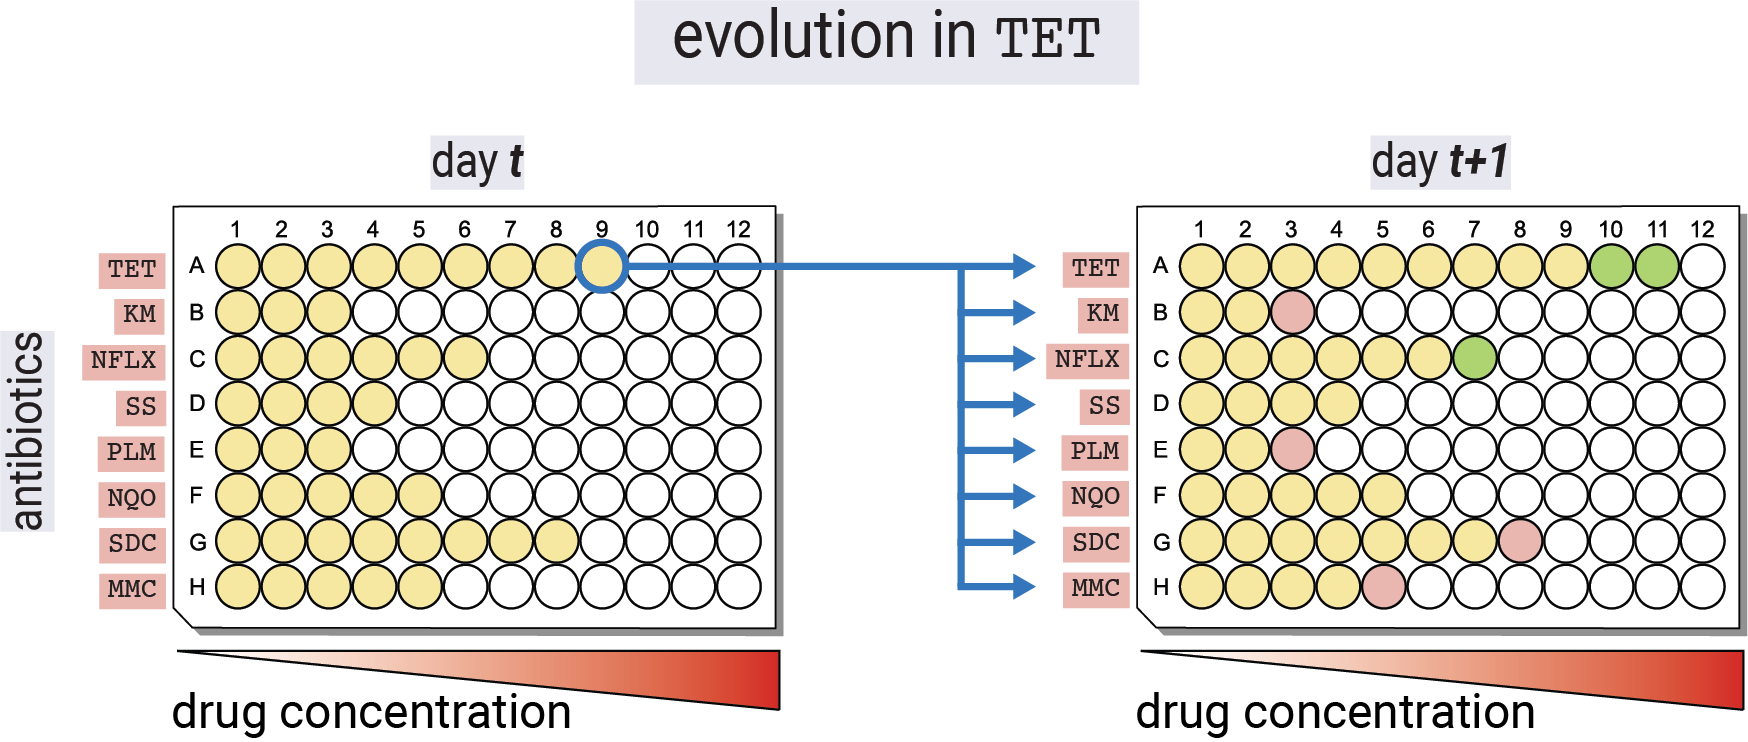
\includegraphics[keepaspectratio]{./fig/supplementary/figSI_iwasawa_experiment.pdf}}

}

\caption{\label{fig-iwasawa-design}\textbf{Iwasawa et al.~experimental
design.} Schematic of the experimental design used by Iwasawa et al.
\autocite{iwasawa2022}. On a 96-well plate, each of the eight rows
contained a titration of one of eight antibiotics. For strains evolved
in tetracycline (\texttt{TET}), the plate for each day \(t+1\) was
inoculated by propagating from the well with the highest tetracycline
concentration in which there was still measurable growth on day \(t\) to
all 96 wells.}

\end{figure}%

Figure~\ref{fig-ic50-progression} shows a typical progression of the
optical density curves over the course of the experimental evolution.
When adapted to a particular antibiotic, the optical density curves with
their sigmoidal shape shifted to the right, indicating that the strains
were able to grow at higher concentrations of the antibiotic.

\begin{figure}

\centering{

\pandocbounded{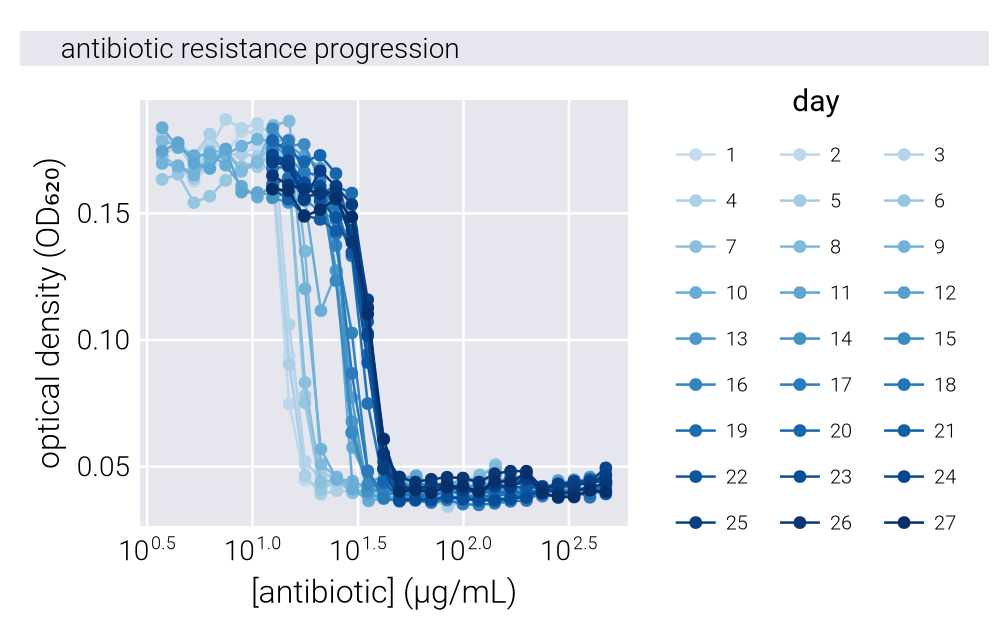
\includegraphics[keepaspectratio]{./fig/supplementary/figSI_ic50_progression.pdf}}

}

\caption{\label{fig-ic50-progression}\textbf{Iwasawa et al.~typical
experimental data.} The optical density curves of the bacterial culture
in the evolution antibiotic over the course of the experiment. The
curves are shifted to the right, indicating that the strains were able
to grow at higher concentrations of the antibiotic.}

\end{figure}%

\subsubsection{\texorpdfstring{Bayesian inference of \(IC_{50}\)
values}{Bayesian inference of IC\_\{50\} values}}\label{bayesian-inference-of-ic_50-values}

Given the natural sigmoidal shape of the optical density curves, we can
model the optical density \(OD(x)\) of the bacterial culture as a
function of the antibiotic concentration \(x\). Following the approach
of \autocite{iwasawa2022}, we model the optical density as a function of
the antibiotic concentration \(x\) as

\begin{equation}\phantomsection\label{eq-ic50-model}{
f(x) = \frac{a}
{1+\exp \left[b\left(\log _2 x-\log _2 \mathrm{IC}_{50}\right)\right]} + c
}\end{equation}

where \(a\), \(b\), and \(c\) are nuisance parameters of the model,
\(\mathrm{IC}_{50}\) is the parameter of interest, and \(x\) is the
antibiotic concentration. We can define a function to compute this
model.

Given the model presented in Equation~\ref{eq-ic50-model}, and the data,
our objective is to infer the value of all parameters (including the
nuisance parameters). By Bayes theorem, we write
\begin{equation}\phantomsection\label{eq-bayes-ic50}{
\pi(\mathrm{IC}_{50}, a, b, c \mid \text{data}) = 
\frac{\pi(\text{data} \mid \mathrm{IC}_{50}, a, b, c) 
\pi(\mathrm{IC}_{50}, a, b, c)}
{\pi(\text{data})},
}\end{equation}

where \(\text{data}\) consists of the pairs of antibiotic concentration
and optical density. Let's begin by defining the likelihood function.
For simplicity, we assume each datum is independent and identically
distributed (i.i.d.) and write

\begin{equation}\phantomsection\label{eq-bayes-ic50-likelihood}{
\pi(\text{data} \mid \mathrm{IC}_{50}, a, b, c) = 
\prod_{i=1}^n \pi(d_i \mid \mathrm{IC}_{50}, a, b, c),
}\end{equation}

where \(d_i = (x_i, y_i)\) is the \(i\)-th pair of antibiotic
concentration and optical density, respectively, and \(n\) is the total
number of data points. We assume that our experimental measurements can
be expressed as

\begin{equation}\phantomsection\label{eq-bayes-ic50-likelihood-data}{
y_i = f(x_i, \mathrm{IC}_{50}, a, b, c) + \epsilon_i,
}\end{equation}

where \(\epsilon_i\) is the experimental error. Furthermore, we assume
that the experimental error is normally distributed, i.e.,

\begin{equation}\phantomsection\label{eq-bayes-ic50-likelihood-error}{
\epsilon_i \sim \mathcal{N}(0, \sigma^2),
}\end{equation}

where \(\sigma^2\) is an unknown variance parameter that must be
included in our inference. Notice that we assume the same variance
parameter for all data points since \(\sigma^2\) is not indexed by
\(i\).

Given this likelihood function, we must update our inference on the
parameters as

\begin{equation}\phantomsection\label{eq-bayes-ic50-posterior}{
\pi(\mathrm{IC}_{50}, a, b, c, \sigma^2 \mid \text{data}) = 
\frac{\pi(\text{data} \mid \mathrm{IC}_{50}, a, b, c, \sigma^2) 
\pi(\mathrm{IC}_{50}, a, b, c, \sigma^2)}
{\pi(\text{data})},
}\end{equation}

to include the new parameter \(\sigma^2\). Our likelihood function is
then of the form

\begin{equation}\phantomsection\label{eq-bayes-ic50-likelihood-model}{
y_i \mid \mathrm{IC}_{50}, a, b, c, \sigma^2 \sim 
\mathcal{N}(f(x_i, \mathrm{IC}_{50}, a, b, c), \sigma^2).
}\end{equation}

For the prior, we assume that all parameters are independent and write
\begin{equation}\phantomsection\label{eq-bayes-ic50-prior}{
\pi(\mathrm{IC}_{50}, a, b, c, \sigma^2) = 
\pi(\mathrm{IC}_{50}) \pi(a) \pi(b) \pi(c) \pi(\sigma^2).
}\end{equation}

Let's detail each prior.

\begin{enumerate}
\def\labelenumi{\arabic{enumi}.}
\item
  \(\mathrm{IC}_{50}\): The \(IC_{50}\) is a strictly positive
  parameter. However, we will fit for \(\log_2(\mathrm{IC}_{50})\).
  Thus, we will use a normal prior for \(\log_2(\mathrm{IC}_{50})\).
  This means we have
  \begin{equation}\phantomsection\label{eq-bayes-ic50-prior-ic50}{
  \log_2(\mathrm{IC}_{50}) \sim 
  \mathcal{N}(
   \mu_{\log_2(\mathrm{IC}_{50})}, \sigma_{\log_2(\mathrm{IC}_{50})}^2
  ).
  }\end{equation}
\item
  \(a\): This nuisance parameter scales the logistic function. Again,
  the natural scale for this parameter is a strictly positive real
  number. Thus, we will use a lognormal prior for \(a\). This means we
  have \begin{equation}\phantomsection\label{eq-bayes-ic50-prior-a}{
  a \sim \text{LogNormal}(\mu_a, \sigma_a^2).
  }\end{equation}
\item
  \(b\): This parameter controls the steepness of the logistic function.
  Again, the natural scale for this parameter is a strictly positive
  real number. Thus, we will use a lognormal prior for \(b\). This means
  we have \begin{equation}\phantomsection\label{eq-bayes-ic50-prior-b}{
  b \sim \text{LogNormal}(\mu_b, \sigma_b^2).
  }\end{equation}
\item
  \(c\): This parameter controls the minimum value of the logistic
  function. Since this is a strictly positive real number that does not
  necessarily scale with the data, we will use a half-normal prior for
  \(c\). This means we have
  \begin{equation}\phantomsection\label{eq-bayes-ic50-prior-c}{
  c \sim \text{Half-}\mathcal{N}(0, \sigma_c^2).
  }\end{equation}
\item
  \(\sigma^2\): This parameter controls the variance of the experimental
  error. Since this is a strictly positive real number that does not
  necessarily scale with the data, we will use a half-normal prior for
  \(\sigma^2\). This means we have
  \begin{equation}\phantomsection\label{eq-bayes-ic50-prior-sigma}{
  \sigma^2 \sim \text{Half-}\mathcal{N}(0, \sigma_{\sigma^2}^2).
  }\end{equation}
\end{enumerate}

\paragraph{Residual-based outlier
detection}\label{residual-based-outlier-detection}

To identify and remove outliers from our optical density measurements,
we implemented a residual-based outlier detection method. First, we fit
the logistic model (Equation~\ref{eq-ic50-model}) to the data using a
deterministic least-squares approach. We then computed the residuals
between the fitted model and the experimental measurements. Points with
residuals exceeding a threshold of two standard deviations from the mean
residual were classified as outliers and removed from subsequent
analysis. This approach helped eliminate experimental artifacts while
preserving the underlying sigmoidal relationship between antibiotic
concentration and optical density.

\subsubsection{MCMC sampling of the
posterior}\label{mcmc-sampling-of-the-posterior}

With this setup, we can sample the posterior distribution using Markov
Chain Monte Carlo (MCMC) methods. In particular, we used the
\texttt{Turing.jl} package \autocite{ge2018} implementation of the
No-U-Turn Sampler (NUTS). All code is available in the GitHub repository
for this work. Figure~\ref{fig-ic50-ppc} shows the posterior predictive
checks of the posterior distribution for the \(IC_{50}\) parameter.
Briefly, the posterior predictive checks are a visual method to assess
the fit of the model to the data. The idea is to generate samples from
the posterior distribution and compare them to the data. If the model is
a good fit, the samples should be able to reproduce the data.

The effectiveness of the residual-based outlier detection method is
demonstrated in Figure~\ref{fig-ic50-ppc}, where the posterior
predictive checks show significantly tighter credible intervals after
outlier removal, particularly in regions of high antibiotic
concentration where experimental noise tends to be more pronounced.

\begin{figure}

\centering{

\pandocbounded{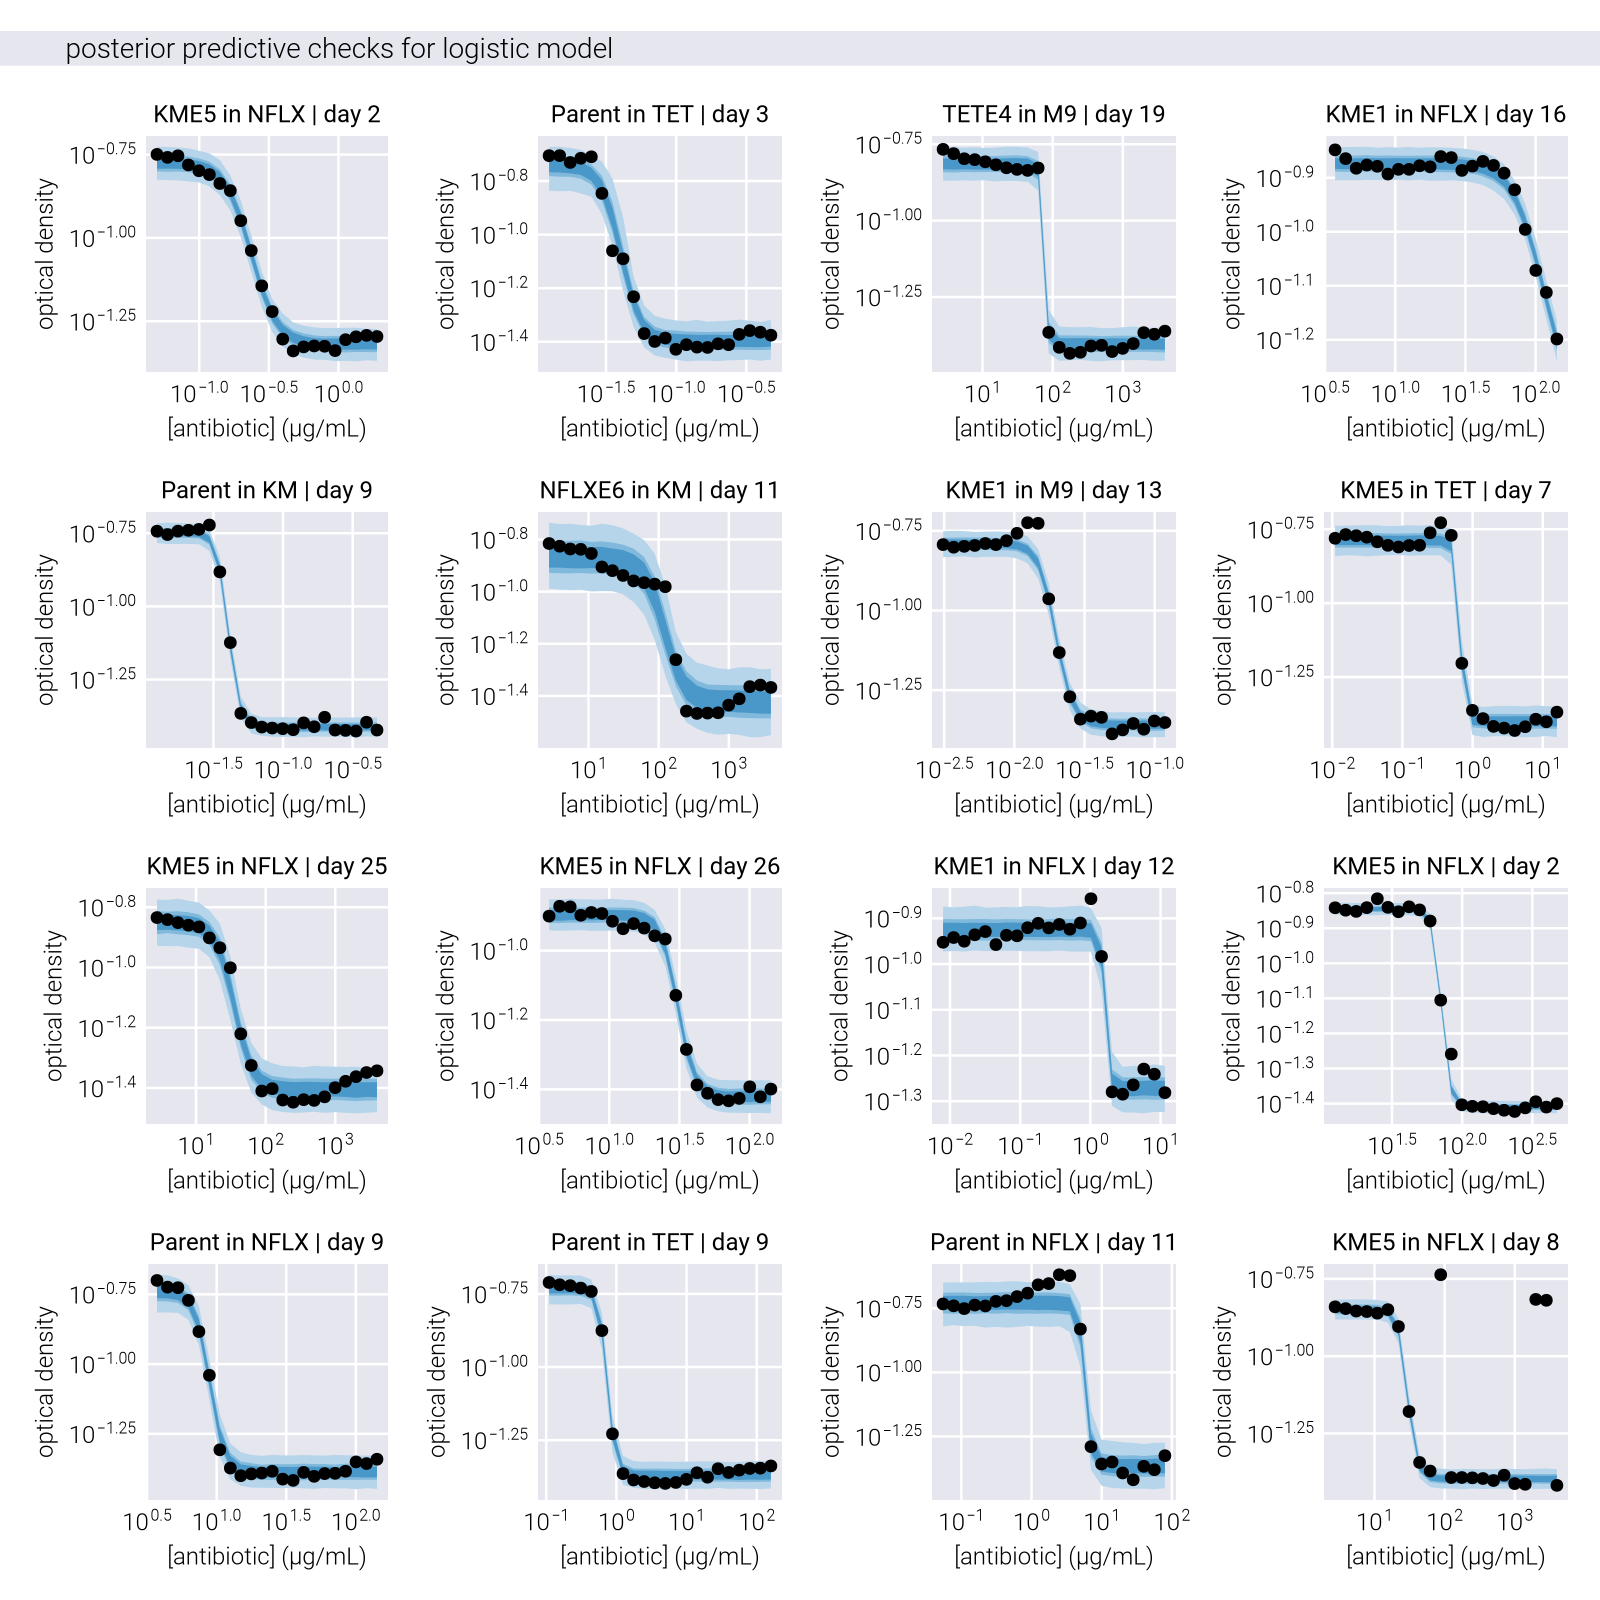
\includegraphics[keepaspectratio]{./fig/supplementary/figSI_ic50_ppc.pdf}}

}

\caption{\label{fig-ic50-ppc}\textbf{Posterior predictive check.} The
posterior predictive check of the posterior distribution for the
\(IC_{50}\) parameter inference. The blue line is the mean of the
posterior distribution, the different shades of blue represent the 95\%,
68\%, and 50\% credible regions. The black dots are the raw optical
density measurements as provided by Iwasawa et al.
\autocite{iwasawa2022}.}

\end{figure}%

\subsection{Metropolis-Hastings Evolutionary
Dynamics}\label{sec-metropolis}

In the main text, we describe a simple algorithm for evolving a
population as a biased random walk on a phenotypic space controlled by
both a fitness function and a genotype-phenotype density function. Here,
we provide a more detailed description of the algorithm and its
implementation.

\subsubsection{Landscape Description}\label{landscape-description}

We assume that phenotypes driving adaptation can be described by
real-valued numbers. Let
\(\underline{x}(t) = (x_1(t), x_2(t), \cdots, x_N(t))\) be an \(N\)
dimensional vector describing the phenotype of a population at time
\(t\). The fitness for a given environment \(E\) is a scalar function
\(F_E(\underline{x})\) such that

\begin{equation}\phantomsection\label{eq-fitnes}{
F_E: \mathbb{R}^N \to \mathbb{R},
}\end{equation}

i.e, the coordinates in phenotype space map to a fitness value.
Throughout this work, we consider a series of Gaussian fitness peaks,
i.e.,

\begin{equation}\phantomsection\label{eq-fitness-peaks}{
F_E(\underline{x}) = 
\sum_{p=1}^P A_p 
\exp\left(
    -\frac{1}{2}
    (\underline{x} - \underline{\hat{x}}^{(p)})^T 
    \Sigma_p^{-1} 
    (\underline{x} - \underline{\hat{x}}^{(p)})
\right),
}\end{equation}

where \(P\) is the number of peaks, \(A_p\) is the amplitude of the
\(p\)-th peak, \(\underline{\hat{x}}^{(p)}\) is the \(N\)-dimensional
vector of optimal phenotypes for the \(p\)-th peak, and \(\Sigma_p\) is
the \(N \times N\) covariance matrix for the \(p\)-th peak. This
formulation allows for multiple peaks in the fitness landscape, each
potentially having different heights, widths, and covariance structures
between dimensions. The covariance matrix \(\Sigma_p\) captures
potential interactions between different phenotypic dimensions, allowing
for more complex and realistic fitness landscapes.

In the same vein, we define a genotype-phenotype density function
\(GP(\underline{x})\) as a scalar function that maps a phenotype to a
mutational effect, i.e.,

\begin{equation}\phantomsection\label{eq-genotype-phenotype-density}{
GP: \mathbb{R}^N \to \mathbb{R},
}\end{equation}

where \(GP(\underline{x})\) is related to the probability of a genotype
mapping to a phenotype \(\underline{x}\). As a particular density
function we will consider a set of negative Gaussian peaks that will
serve as ``mutational barriers'' that limit the range of phenotypes that
can be reached. The deeper the peak, the less probable it is that a
genotype will map to a phenotype within the peak. This idea captured by
the following mutational landscape

\begin{equation}\phantomsection\label{eq-genotype-phenotype-density-peaks}{
GP(\underline{x}) = 
\sum_{p=1}^P -B_p 
\exp\left(
    -\frac{1}{2}
    (\underline{x} - \underline{\hat{x}}^{(p)})^T 
    \Sigma_p^{-1} 
    (\underline{x} - \underline{\hat{x}}^{(p)})
\right),
}\end{equation}

where \(B_p\) is the depth of the \(p\)-th peak, and
\(\underline{\hat{x}}^{(p)}\) is the \(N\)-dimensional vector of optimal
phenotypes for the \(p\)-th peak.

\subsubsection{Metropolis-Hastings
Algorithm}\label{metropolis-hastings-algorithm}

The Metropolis-Hastings algorithm is a Markov Chain Monte Carlo (MCMC)
method used to sample from a target probability distribution
\(\pi(\underline{x})\). In our evolutionary context,
\(\pi(\underline{x})\) can be thought of as the steady-state
distribution of phenotypes under the combined influence of selection and
mutation. We can define this distribution as

\begin{equation}\phantomsection\label{eq-metropolis-hastings-target-distribution}{
\pi(\underline{x}) \propto \exp\left(
    -\beta U(\underline{x})
\right),
}\end{equation}

where \(U(\underline{x})\) is the potential function defined as

\begin{equation}\phantomsection\label{eq-metropolis-hastings-potential-function}{
U(\underline{x}) = \ln F_E(\underline{x}) + \ln GP(\underline{x}).
}\end{equation}

This functional form of the potential function is motivated by the
desired property of the potential function being a sum of the fitness
and genotype-phenotype density functions. \(\beta\) in
Equation~\ref{eq-metropolis-hastings-target-distribution} is an inverse
temperature parameter (from statistical mechanics) that controls the
level of stochasticity in the system. A higher \(\beta\) means the
system is more likely to move towards higher fitness and
genotype-phenotype density. In a sense, \(\beta\) can be related to the
effective population size, controlling the directness of the
evolutionary dynamics.

At each step, we propose a new phenotype \(\underline{x}{\prime}\) from
a proposal distribution \(q(\underline{x}{\prime} | \underline{x})\).
For simplicity, we can use a symmetric proposal distribution, such as a
Gaussian centered at the current phenotype. Further, we constrain the
proposal distribution to be symmetric, i.e.,

\begin{equation}\phantomsection\label{eq-metropolis-hastings-proposal-distribution-symmetry}{
q(\underline{x}{\prime} | \underline{x}) = 
q(\underline{x} | \underline{x}{\prime}).
}\end{equation}

This symmetry simplifies the acceptance probability later on.

The acceptance probability \(P_{\text{accept}}\) for moving from
\(\underline{x}\) to \(\underline{x}{\prime}\) is given by

\begin{equation}\phantomsection\label{eq-metropolis-hastings-acceptance-probability}{
P_{\text{accept}} = 
\min\left(1, 
    \frac{\pi(\underline{x}{\prime}) q(\underline{x} | \underline{x}{\prime})}
    {\pi(\underline{x}) q(\underline{x}{\prime} | \underline{x})}
\right).
}\end{equation}

Given the symmetry of the proposal distribution,
\(q(\underline{x}{\prime} |
\underline{x}) = q(\underline{x} | \underline{x}{\prime})\) , so the
acceptance probability simplifies to

\begin{equation}\phantomsection\label{eq-metropolis-hastings-acceptance-probability-simplified}{
P_{\text{accept}} = \min\left(
    1, 
    \frac{\pi(\underline{x}{\prime})}{\pi(\underline{x})}
    \right).
}\end{equation}

Substituting Equation~\ref{eq-metropolis-hastings-target-distribution}
and Equation~\ref{eq-metropolis-hastings-potential-function} into
Equation~\ref{eq-metropolis-hastings-acceptance-probability-simplified},
we get:

\begin{equation}\phantomsection\label{eq-metropolis-hastings-acceptance-probability-simplified-2}{
P_{\text{accept}} = \min\left(
    1, 
    e^{\beta [\ln F_E(\underline{x}{\prime}) + \ln M(\underline{x}{\prime})] - 
    \beta [\ln F_E(\underline{x}) + \ln M(\underline{x})]}
    \right).
}\end{equation}

This can be rewritten as

\begin{equation}\phantomsection\label{eq-acceptance}{
P_{\text{accept}} = \min\left(
    1,
    \frac{F_E(\underline{x}{\prime})^β GP(\underline{x}{\prime})^β}
    {F_E(\underline{x})^β GP(\underline{x})^β}
\right),
}\end{equation}

This expression shows that the acceptance probability depends on the
difference in fitness and genotype-phenotype density between the current
and proposed phenotypes.

\subsubsection{Effect of Inverse
Temperature}\label{effect-of-inverse-temperature}

Figure~\ref{fig-metropolis-inverse-temperature} shows the effect of the
inverse temperature parameter \(\beta\) influences evolutionary
trajectories in our Metropolis-Hastings framework. Through a series of
panels showing both phenotypic trajectories (upper) and fitness dynamics
(lower), we can observe how different \(\beta\) values affect the
balance between exploration and exploitation in phenotypic space.

At low \(\beta\) values (left panels), the evolutionary trajectories
exhibit highly stochastic behavior, with populations taking meandering
paths through the phenotypic landscape. This represents a regime where
genetic drift plays a dominant role. As \(\beta\) increases (moving
right), the trajectories become increasingly deterministic, with
populations taking more direct paths toward fitness peaks, while
avoiding genotype-to-phenotype density valleys. This transition reflects
a shift from drift-dominated to selection-dominated dynamics, where
populations more strictly follow the local fitness gradient. The fitness
trajectories in the lower panels further reinforce this pattern, showing
more erratic fitness fluctuations at low \(\beta\) and more monotonic
increases at high \(\beta\), consistent with stronger selective
pressures.

\begin{figure}

\centering{

\pandocbounded{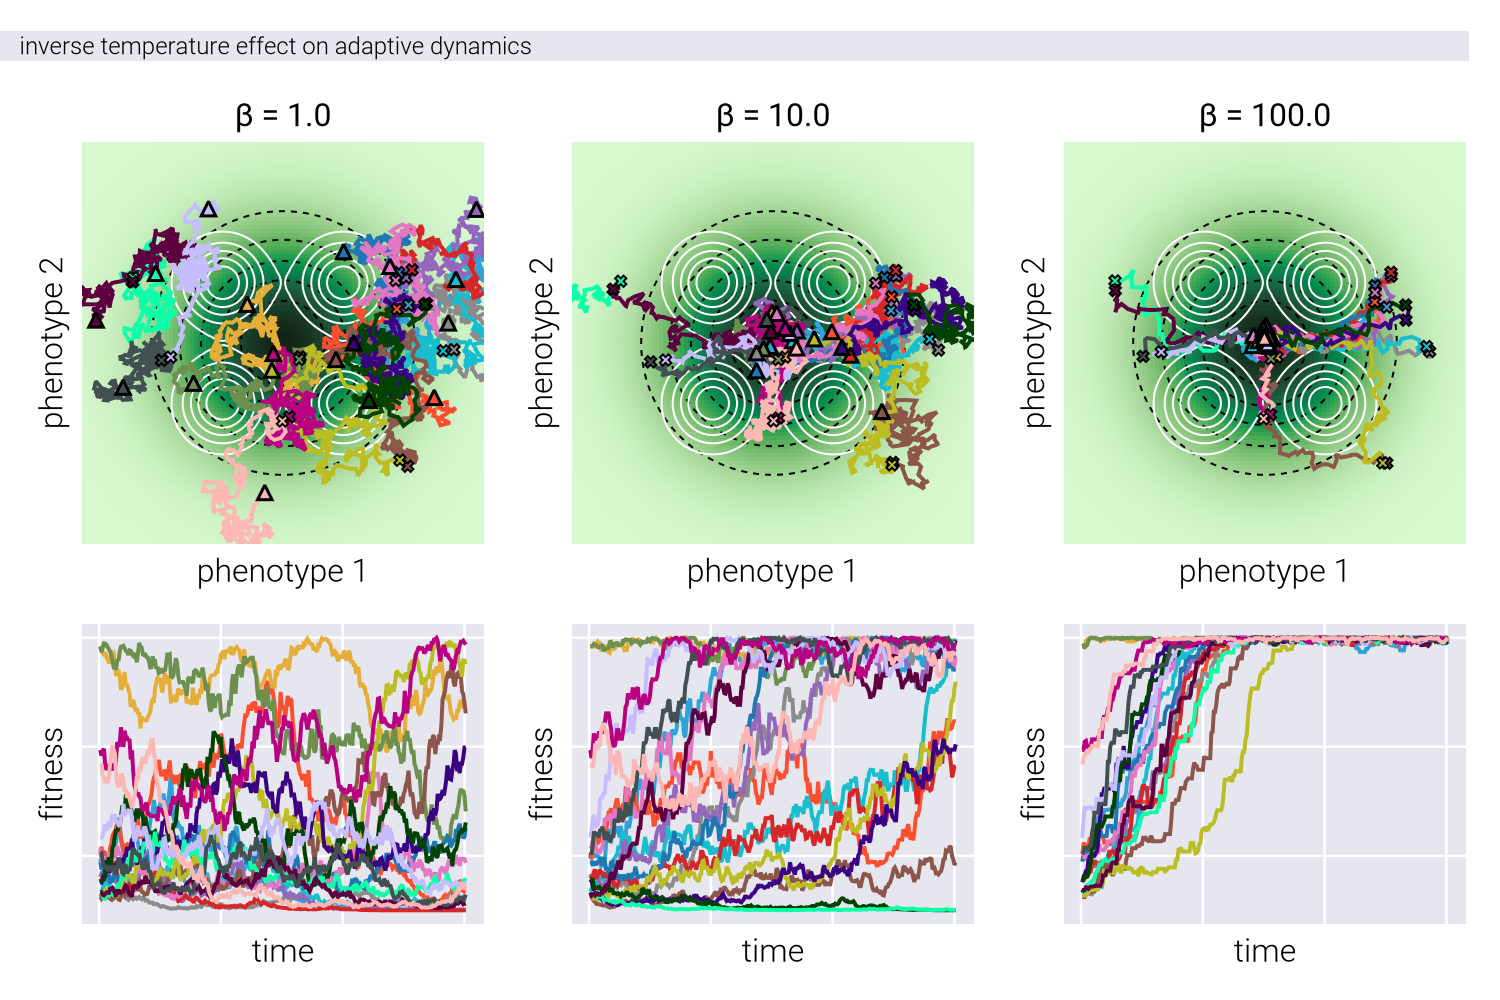
\includegraphics[keepaspectratio]{./fig/supplementary/figSI_sim_beta_effect.pdf}}

}

\caption{\label{fig-metropolis-inverse-temperature}\textbf{Effect of
inverse temperature on adaptive dynamics}. Upper panels: Population
trajectories on a landscape with a single fitness peak and four
genotype-phenotype density peaks. Black dashed lines indicate fitness
landscape contours, while white solid lines show genotype-phenotype
density contours. Colored lines represent independent population
trajectories, with initial positions (crosses) and final positions
(triangles). Lower panels: Temporal evolution of population fitness.
Panels from left to right show increasing values of inverse temperature
(\(\beta\)), demonstrating increasingly deterministic adaptive
trajectories.}

\end{figure}%

\subsection{Riemannian Hamiltonian Variational Autoencoders Mathematical
Background}\label{riemannian-hamiltonian-variational-autoencoders-mathematical-background}

The bulk of this work makes use of the variational autoencoder variation
developed by \autocite{chadebec2020} known as Riemannian Hamiltonian
Variational Autoencoder (RHVAE). Understanding this model requires some
background that we provide in the following sections. It is not
necessary to follow every mathematical derivation in detail for these
sections, as they don't directly pertain to the main contribution of
this work. However, we believe that some intuition behind some of the
concepts that inspired the RHVAE model can go a long way to understand
the model. We invite the reader to refer to the original paper
\autocite{chadebec2020} and the references therein for additional
details.

Let us start by reviewing the variational autoencoder model setting and
the variational inference framework.

\subsubsection{Variational Autoencoder Model
Setting}\label{variational-autoencoder-model-setting}

Given a data set
\(\underline{x}^{1:N} \in \mathcal{X} \subseteq \mathbb{R}^D\), where
the superscript denotes a set of \(N\) observations, i.e.,
\begin{equation}\phantomsection\label{eq-data-set}{
\underline{x}^{1:N} = 
\left\{
    \underline{x}_1, \underline{x}_2, \ldots, \underline{x}_N
\right\},
}\end{equation} where \(\underline{x}_i \in \mathbb{R}^D\) for
\(i = 1, 2, \ldots, N\), the variational autoencoder aims to fit a joint
distribution \(π_\theta(\underline{x}, \underline{z})\) where the data
generative process is assumed to involve a set of
latent---unobserved---continuous variables
\(\underline{z} \in \mathcal{Z} \subseteq \mathbb{R}^d\), where usually
\(d \ll D\). In other words, the VAE assumes that the data we get to
observe is a consequence of a set of hidden variables \(\underline{z}\)
that we cannot measure directly. We assume that these variables live in
a much lower-dimensional space than the one we observe and we are trying
to learn this joint distribution such that, if desired, we can generate
new data points by sampling from this distribution. Since the data we
observe is a ``consequence'' of the latent variables, we express this
joint distribution as

\begin{equation}\phantomsection\label{eq-joint-dist}{
π_\theta(\underline{x}, \underline{z}) = 
π_\theta(\underline{x}|\underline{z}) \, π_\text{prior}(\underline{z}),
}\end{equation}

where \(π_\text{prior}(\underline{z})\) is the prior distribution over
latent variables and \(π_\theta(\underline{x}|\underline{z})\) is the
likelihood of the data given the latent variables. This looks exactly as
the problem one confronts when performing Bayesian inference. What
distinguishes the VAE from other Bayesian inference problems, as we will
see, is that in many cases, we do not know the functional form of both
the prior and the likelihood function that generated our data, but we
have enough data samples that we hope to be able to learn these function
using the neural networks function approximation capabilities. Thus, the
objective of the VAE is to parameterize this likelihood function via a
neural network with parameters \(\theta\) given some prior distribution
over the latent variables. For simplicity, it is common to choose a
standard normal prior distribution, i.e.,
\(π_\text{prior}(\underline{z}) =
\mathcal{N}(\underline{0}, \underline{\underline{I}}_d)\), where
\(\underline{\underline{I}}_d\) is the \(d\)-dimensional identity matrix
\autocite{kingma2014a,kingma2019}. This way, once we have learned the
parameters of the neural network, we can generate new data points by
sampling from this prior distribution and running the resulting samples
through the likelihood function encoded by this neural network.

Our objective then becomes to find the parameters \(\theta\) that
maximize the probability of observing the data we actually observed.
This is equivalent to maximizing the so-called marginal likelihood of
the data, i.e.,

\begin{equation}\phantomsection\label{eq-marginal-likelihood}{
\max_\theta \, π_\theta(\underline{x}) = 
\max_\theta \int d^d\underline{z} \, π_\theta(\underline{x}, \underline{z}).
}\end{equation}

But there are two problems with this objective:

\begin{enumerate}
\def\labelenumi{\arabic{enumi}.}
\tightlist
\item
  The marginalization over the latent variables is intractable for most
  interesting distributions.
\item
  The distribution \(π_\theta(\underline{x})\) is in general unknown and
  we need to somehow approximate it.
\end{enumerate}

The way around these problems is to introduce a family of parametric
distributions \(q_\phi(\underline{z} \mid \underline{x})\), i.e.,
distributions that can be completely characterized by a set of
parameters (think of Gaussians being a parametric family on the mean and
the variance), and to approximate the true marginal distribution with
one of these parametric distributions. This conceptual change is at the
core of approximate methods for Bayesian inference known as variational
inference. The objective then becomes to find the parameters \(\phi\)
that, when used to approximate the posterior distribution
\(π_\theta(\underline{z}|\underline{x})\), it is as close as possible to
this posterior distribution. To mathematize this objective, we establish
that we want to minimize the Kullback-Leibler divergence (also known as
the relative entropy) between the variational distribution
\(q_\phi(\underline{z} \mid \underline{x})\) and the posterior
distribution \(π_\theta(\underline{z} \mid \underline{x})\), i.e., we
aim to find \(q_\phi^*\) such that

\begin{equation}\phantomsection\label{eq-variational-approx}{
q_\phi^*(\underline{z} \mid \underline{x}) = 
\min_\phi \, D_{KL}\left(
    q_\phi(\underline{z} \mid \underline{x}) \| 
    π_\theta(\underline{z} \mid \underline{x})
\right).
}\end{equation}

After some algebraic manipulation involving the well-known Gibbs
inequality, we can show that this objective is equivalent to maximizing
the so-called evidence lower bound (ELBO), \(\mathcal{L}\), of the
marginal likelihood, i.e.,

\begin{equation}\phantomsection\label{eq-elbo}{
\mathcal{L} = \left\langle 
    \log π_\theta(\underline{x}, \underline{z}) - 
    \log q_\phi(\underline{z} \mid \underline{x}) 
\right\rangle_{q_\phi} 
\leq \log π_\theta(\underline{x}).
}\end{equation}

Thus, the optimization problem we want to solve invovles estimating the
ELBO given some data \(\underline{x}\). However, the ELBO is an
expectation over the variational distribution
\(q_\phi(\underline{z} \mid \underline{x})\), which is unknown.
Therefore, we need to somehow estimate this expectation. Arguably, the
most important contribution of the VAE framework is the introduction of
the reparametrization trick \autocite{kingma2014a}. This seemingly
innocuous trick allows us to compute an unbiased estimate of the ELBO
and its gradient, such that we can maximize it via gradient ascent. For
more details on the reparametrization trick, we refer the reader to
\autocite{kingma2014a}.

More recent attempts have focused on modifying
\(q_\phi(\underline{z} \mid
\underline{x})\) to get a better approximation of the true posterior
\(π_\theta(\underline{z} \mid \underline{x})\). The basis of the
Riemannian Hamiltonian Variational Autoencoder (RHVAE) framework takes
inspiration from some of these approaches. Let's gain some intuition on
each of them.

\subsubsection{MCMC and VI (Salimans \& Kingma
2015)}\label{mcmc-and-vi-salimans-kingma-2015}

One such approach to improve the accuracy of the variational posterior
approximation consists in adding a fix number of Markov Chain Monte
Carlo (MCMC) steps to the variational posterior approximation, targeting
the true posterior \autocite{salimans2015}. In MCMC, rather than
optimizing the parameters of a parametric distribution, we sample an
initial position \(\underline{z}_0\) from a simple distribution
\(q(\underline{z}_0)\) or \(q(\underline{z}_0 \mid \underline{x})\) and
subsequently, apply a stochastic transition operator
\(T(\underline{z}_{t+1} \mid
\underline{z}_t)\) to draw a new value \(\underline{z}_{t+1}\) from the
distribution

\begin{equation}\phantomsection\label{eq-mcmc-transition}{
\underline{z}_{t + 1} \sim T(\underline{z}_{t+1} \mid \underline{z}_t).
}\end{equation}

Applying this operator over and over again, we build a Markov chain

\begin{equation}\phantomsection\label{eq-mcmc-chain}{
\underline{z}_0 \to \underline{z}_1 \to \underline{z}_2 \to \cdots 
\to \underline{z}_\tau,
}\end{equation}

whose long-term behavior---the so-called stationary distribution---is a
very good approximation of the true posterior distribution
\(π_\theta(\underline{z}
\mid \underline{x})\). In other words, by carefully engineering the
transition operator \(T(\underline{z}_{t+1} \mid \underline{z}_t)\), and
applying it over and over again, the ``histogram'' of the samples
\(\{\underline{z}_t\}_{t=0}^\tau\) will converge to the true posterior
distribution \(π_\theta(\underline{z} \mid
\underline{x})\).

The central idea to combine MCMC with variational inference is to
interpret the Markov chain

\begin{equation}\phantomsection\label{eq-mcmc-chain-def}{
q_\phi(\underline{z} | \underline{x}) = 
q_\phi(\underline{z}_0 \mid \underline{x}) 
\prod_{t=1}^\tau T(\underline{z}_t \mid \underline{z}_{t-1}, \underline{x})
}\end{equation}

as a variational approximation in an expanded space of variables that
includes the original latent variables \(\underline{z}\) and the
auxiliary variables
\(\underline{Z} = \{\underline{z}_0, \underline{z}_1, \ldots,
\underline{z}_{\tau-1}\}\). Note that \(\underline{Z}\) reaches up to
\(\tau-1\) steps, since we consider the final step
\(\underline{z}_\tau\) to be the original latent variable
\(\underline{z}\). In other words, our variational distribution now
writes
\begin{equation}\phantomsection\label{eq-mcmc-chain-def-expanded}{
q_\phi(\underline{z}_\tau, \underline{Z} \mid \underline{x}) = 
q_\phi(\underline{z}_0 \mid \underline{x}) 
\prod_{t=1}^\tau T(\underline{z}_t \mid \underline{z}_{t-1}, \underline{x}).
}\end{equation}

Integrating this expression into the ELBO (Equation~\ref{eq-elbo})
consists of substituting the variational distribution
\(q_\phi(\underline{z} \mid \underline{x})\) with the expression in
Equation~\ref{eq-mcmc-chain-def-expanded}, i.e.,
\begin{equation}\phantomsection\label{eq-elbo-aux}{
\mathcal{L}_{\text {aux }} =
\left\langle\log 
    \left[
        \pi_\theta\left(\underline{x}, \underline{z}_T\right) 
        r\left(\underline{Z} \mid \underline{z}_T, \underline{x}\right)
    \right] - 
    \log q\left(\underline{Z}, \underline{z}_T \mid \underline{x}\right)
\right\rangle_{q\left(\underline{Z}, \underline{z}_T \mid \underline{x}\right)}
}\end{equation}

where \(r(\underline{Z} \mid \underline{z}_T, \underline{x})\) is an
auxiliary inference distribution that we can choose freely. This
auxiliary distribution is necessary to ensure we account for the
auxiliary variables \(\underline{Z}\) that are now part of our
variational distribution. By splitting the joint distribution in
Equation~\ref{eq-mcmc-chain-def-expanded} as

\begin{equation}\phantomsection\label{eq-mcmc-chain-def-expanded-2}{
q_\phi(\underline{z}_\tau, \underline{Z} \mid \underline{x}) =
q_\phi(\underline{Z} \mid \underline{z}_\tau, \underline{x}) q_\phi(\underline{z}_\tau \mid \underline{x}),
}\end{equation}

and substituting this expression into Equation~\ref{eq-elbo-aux}, we get

\begin{equation}\phantomsection\label{eq-elbo-aux-2}{
\mathcal{L}_{\text {aux }} =
\left\langle\log 
    \left[
        \pi_\theta\left(\underline{x}, \underline{z}_T\right) 
        r\left(\underline{Z} \mid \underline{z}_T, \underline{x}\right)
    \right] - 
    \log \left[q_\phi(\underline{Z} \mid \underline{z}_\tau, \underline{x}) q_\phi(\underline{z}_\tau \mid \underline{x})\right]
\right\rangle_{q_\phi(\underline{Z} \mid \underline{z}_\tau, \underline{x}) q_\phi(\underline{z}_\tau \mid \underline{x})}.
}\end{equation}

Rearranging the terms, we get
\begin{equation}\phantomsection\label{eq-elbo-aux-3}{
\begin{aligned}
\mathcal{L}_{\text {aux }} 
& = \left\langle 
    \log \frac{\pi_\theta\left(\underline{x}, \underline{z}_\tau\right)}{q_\phi(\underline{z}_\tau \mid \underline{x})} - 
    \log \frac{q_\phi(\underline{Z} \mid \underline{z}_\tau, \underline{x})}{r(\underline{Z} \mid \underline{z}_\tau, \underline{x})}
\right\rangle_{
    q_\phi(\underline{Z} \mid \underline{z}_\tau, \underline{x})
    q_\phi(\underline{z}_\tau \mid \underline{x})
}, \\
& = \left\langle 
    \log \frac{\pi_\theta\left(\underline{x}, \underline{z}_\tau\right)}{q_\phi(\underline{z}_\tau \mid \underline{x})}
\right\rangle_{
    q_\phi(\underline{Z} \mid \underline{z}_\tau, \underline{x})
    q_\phi(\underline{z}_\tau \mid \underline{x})
} - 
\left\langle
    \log \frac{q_\phi(\underline{Z} \mid \underline{z}_\tau, \underline{x})}{r(\underline{Z} \mid \underline{z}_\tau, \underline{x})}
\right\rangle_{
    q_\phi(\underline{Z} \mid \underline{z}_\tau, \underline{x})
    q_\phi(\underline{z}_\tau \mid \underline{x})
}.
\end{aligned}
}\end{equation}

From here, we note that the first term in Equation~\ref{eq-elbo-aux-3}
is the original ELBO with the extra expectation taken over the auxiliary
variables \(\underline{Z}\). However, this term does not depend on the
auxiliary variables \(\underline{Z}\), thus, we can take it out of the
expectation, i.e.,

\begin{equation}\phantomsection\label{eq-elbo-aux-4}{
\mathcal{L}_{\text {aux }} = \mathcal{L} - 
\left\langle 
    \log \frac{q_\phi(\underline{Z} \mid \underline{z}_\tau, \underline{x})}{r(\underline{Z} \mid \underline{z}_\tau, \underline{x})}
\right\rangle_{
    q_\phi(\underline{Z} \mid \underline{z}_\tau, \underline{x})
    q_\phi(\underline{z}_\tau \mid \underline{x})
}.
}\end{equation}

For the second term, taking the expectation over the auxiliary variables
makes it equivalent to the KL divergence between the variational
distribution
\(q_\phi(\underline{Z} \mid \underline{z}_\tau, \underline{x})\) and the
auxiliary distribution
\(r(\underline{Z} \mid \underline{z}_\tau, \underline{x})\), i.e.,

\begin{equation}\phantomsection\label{eq-elbo-aux-5}{
\mathcal{L}_{\text {aux }} = \mathcal{L} - 
\left\langle 
    D_{K L}\left[
        q\left(\underline{Z} \mid \underline{z}_T, \underline{x}\right) \| 
        r\left(\underline{Z} \mid \underline{z}_T, \underline{x}\right)
    \right]
\right\rangle_{q\left(\underline{z}_T \mid \underline{x}\right)}
\leq \mathcal{L} \leq \log [\pi_\theta(\underline{x})].
}\end{equation}

where the inequality follows from the non-negativity of the KL
divergence and the fact that the ELBO is a lower bound to the marginal
likelihood. Since the variational distribution
\(q_\phi(\underline{z}_\tau,\mid \underline{x})\) we care about comes
from the marginalization of the variational distribution over the
auxiliary variables \(\underline{Z}\),

\begin{equation}\phantomsection\label{eq-mcmc-marginalization}{
q_\phi(\underline{z}_\tau \mid \underline{x}) = 
\int d\underline{Z} \, 
q_\phi(\underline{Z}, \underline{z}_\tau \mid \underline{x}),
}\end{equation}

it is now a very rich family of distributions that can be used to better
approximate the true posterior distribution
\(π_\theta(\underline{z} \mid
\underline{x})\). However, we are still left with the task of choosing
the auxiliary distribution \(r(\underline{Z} \mid \underline{z}_\tau,
\underline{x})\). What Salimans \& Kingma \autocite{salimans2015}
propose is to define this distribution also as a Markov chain, but in
reverse order, i.e.,

\begin{equation}\phantomsection\label{eq-mcmc-chain-def-aux}{
r(\underline{Z} \mid \underline{z}_\tau, \underline{x}) = 
\prod_{t=1}^\tau 
T^\dagger(\underline{z}_{t-1} \mid \underline{z}_t, \underline{x}),
}\end{equation}

where
\(T^\dagger(\underline{z}_{t-1} \mid \underline{z}_t, \underline{x})\)
is the reverse of the transition operator \(T(\underline{z}_{t+1} \mid
\underline{z}_t, \underline{x})\). Notice that the dependence on
\(\underline{z}_\tau\) is dropped.

This choice of the auxiliary distribution leads to an upper bound on the
marginal log likelihood, of the form

\begin{equation}\phantomsection\label{eq-elbo-aux-6}{
\begin{aligned}
\log \pi_\theta(\underline{x}) & \geq 
\left\langle
    \log \pi_\theta\left(\underline{x}, \underline{z}_\tau\right) -
    \log q_\phi\left(
        \underline{z}_0, \ldots, \underline{z}_\tau \mid \underline{x}
    \right) +
    \log r\left(
        \underline{z}_0, \ldots, \underline{z}_{\tau-1} \mid \underline{x}, \underline{z}_\tau
    \right)
\right\rangle_{q_\phi} \\
& = \left\langle
    \log \left[\frac{
        \pi_\theta\left(\underline{x}, \underline{z}_\tau\right)
        }{
            q_\phi\left(\underline{z}_0 \mid \underline{x}\right)
        }
    \right] +
    \sum_{t=1}^\tau \log \left[
        \frac{
            T^\dagger\left(\underline{z}_{t-1} \mid \underline{z}_t, \underline{x}\right)
        }{
            T\left(\underline{z}_t \mid \underline{z}_{t-1}, \underline{x}\right)
        }
    \right]
\right\rangle_{q_\phi}.
\end{aligned}
}\end{equation}

In other words, we can interpret the Markov chain as a parametric
distribution over the latent variables \(\underline{z}\) that we can use
to approximate the true posterior distribution
\(π_\theta(\underline{z} \mid \underline{x})\). The unbiased estimator
of the marginal likelihood is then given by

\begin{equation}\phantomsection\label{eq-mcmc-approx}{
\hat{π}_\theta(\underline{x}) = 
\frac{
    π_\theta(\underline{x}, \underline{z}_T) 
    \prod_{t=1}^T T^\dagger(\underline{z}_{t-1} \mid \underline{z}_t, \underline{x})
}{
    q_\phi(\underline{z}_0 \mid \underline{x}) 
    \prod_{t=1}^T T(\underline{z}_t \mid \underline{z}_{t-1}, \underline{x})
}.
}\end{equation}

Let's unpack this expression. When performing MCMC, we build a Markov
chain

\begin{equation}\phantomsection\label{eq-mcmc-chain}{
\underline{z}_0 \to \underline{z}_1 \to \underline{z}_2 \to \cdots 
\to \underline{z}_T,
}\end{equation}

where \(\underline{z}_0 \sim q_\phi(\underline{z} \mid \underline{x})\)
is the initial position in the chain. At each step, we sample a new
position from the transition kernel
\(T(\underline{z}_{t} \mid \underline{z}_{t-1},
\underline{x})\), which is a function of the current position and the
observed data. This way, we build a Markov chain that converges to the
true posterior distribution. Therefore, the denominator of
Equation~\ref{eq-mcmc-approx} computes the probability of the initial
position of the chain \(q_\phi(\underline{z}_0 \mid
\underline{x})\) times the product of the transition probabilities for
each of the \(\tau\) steps, \(\prod_{t=1}^\tau T(\underline{z}_{t} \mid
\underline{z}_{t-1}, \underline{x})\).

The numerator of Equation~\ref{eq-mcmc-approx} computes the equivalent
probability, but in reverse order, i.e., starts by sampling the final
position of the chain \(\underline{z}_T\) from the joint distribution
\(π_\theta(\underline{x},
\underline{z}_T)\) and then samples the previous positions of the chain
\(\underline{z}_{T-1}, \underline{z}_{T-2}, \ldots, \underline{z}_0\)
from the transition kernel run backwards,
\(T^\dagger(\underline{z}_{t-1} \mid
\underline{z}_{t}, \underline{x})\). Including a Markov chain into the
variational posterior approximation has the effect of trading off
computational efficiency for better posterior approximation. In other
words, to improve the quality of the posterior approximation we make use
of arguably the most accurate family of inference methods known to
date---Markov Chain Monte Carlo (MCMC)---at the cost of increased
computational cost. Intuitively, our estimate of the unbiased gradient
of the ELBO becomes more and more accurate the more steps we include in
the Markov chain, but at the same time, the cost of computing this
gradient becomes higher and higher.

\subsubsection{Normalizing Flows (Rezende \& Mohamed
2015)}\label{sec-normalizing-flows}

Another approach to imrpove the posterior approximation is to consider
the composition of simple smooth invertible transformations
\autocite{rezende2016}, such that a variable \(\underline{z}_K\)
consists of \(K\) of such transformations of a random variable
\(\underline{z}_0\), sampled from a simple distribution, i.e.,
\(\underline{z}_K\) is built from chaining \(K\) simple transformations,
\(f_x^k\), of \(\underline{z}_0\),

\begin{equation}\phantomsection\label{eq-normalizing-flow}{
\underline{z}_K = 
f_x^K \circ f_x^{K-1} \circ \cdots \circ f_x^1(\underline{z}_0),
}\end{equation}

where \(f_i \circ f_j(x) = f_i(f_j(x))\). Because we define the
transformations to be smooth and invertible, the change of variables
formula tells us that the density of \(\underline{z}_K\) writes

\begin{equation}\phantomsection\label{eq-flow-density}{
q_\phi(\underline{z}_K \mid \underline{x}) = 
q_\phi(\underline{z}_0 \mid \underline{x}) \prod_{k=1}^K |\det J_{f_x^k}|^{-1},
}\end{equation}

where

\begin{equation}\phantomsection\label{eq-jacobian}{
J_{f_x^k} = \frac{\partial f_x^k}{\partial \underline{z}},
}\end{equation}

is the Jacobian matrix of the transformation \(f_x^k\). In other words,
the transformation of the random variable upon a composition of simple
transformations is a product of the Jacobians of each transformation.
Thus, if we choose a sequence of simple transformations, with a simple
Jacobian matrix, we can construct a more complex distribution over the
latent variables. Again, this has the effect of trading off
computational efficiency for better posterior approximation, this time
in the form of smooth invertible transformations of the original
variational distribution. In other words, say that approximating the
posterior distribution using a simple distribution, such as a Gaussian,
is too simple. We can use a sequence of smooth invertible
transformations to transform this simple distribution into a more
complex one that can better approximate the true posterior. This again,
comes at the cost of increased computational cost.

\subsubsection{Hamiltonian Markov Chain Monte Carlo
(HMC)}\label{hamiltonian-markov-chain-monte-carlo-hmc}

Although seemingly unrelated to the previous two approaches, the
Hamiltonian Markov Chain Monte Carlo (HMC) framework provides a way to
construct a Markov chain that is informed by the target distribution we
are trying to approximate. This property is exploited by the predecessor
of the RHVAE framework, the Hamiltonian Variational Autoencoder that we
will review in the next section. But first, let us give a brief overview
of the main ideas of the HMC framework. We direct the interested reader
to the excellent review \autocite{betancourt2017} for a more detailed
treatment of the topic.

In the HMC framework, a random variable \(\underline{z}\) is assumed to
live in an Euclidean space with a target density
\(π(\underline{z} \mid \underline{x})\) derived from a potential
\(U_{\underline{x}}(\underline{z})\), such that the distribution writes

\begin{equation}\phantomsection\label{eq-hmc-dist}{
π(\underline{z} \mid \underline{x}) = 
\frac{e^{-U_{\underline{x}}(\underline{z})}}
{\int d^d\underline{z} \, e^{-U_{\underline{x}}(\underline{z})}},
}\end{equation}

where we define the potential energy as

\begin{equation}\phantomsection\label{eq-potential-energy}{
U_{\underline{x}}(\underline{z}) \equiv -\log π(\underline{z} \mid \underline{x}).
}\end{equation}

Notice that upon substitution of this definition into
Equation~\ref{eq-hmc-dist}, we get the trivial equality

\begin{equation}\phantomsection\label{eq-trivial-equality}{
π(\underline{z} \mid \underline{x}) = 
\frac{\exp[-(-\log π(\underline{z} \mid \underline{x}))]}
{\int d^d\underline{z} \, \exp[-(-\log π(\underline{z} \mid \underline{x}))]} = 
\frac{
    π(\underline{z} \mid \underline{x})
}{
    \int d^d\underline{z} \, π(\underline{z} \mid \underline{x})
} = 
π(\underline{z} \mid \underline{x}).
}\end{equation}

Since it is most of the time impossible to sample directly from
\(π(\underline{z}
\mid \underline{x})\), an independent auxiliary variable
\(\underline{\rho} \in
\mathbb{R}^d\) is introduced and used to sample \(\underline{z}\) more
efficiently. This variable---referred as the momentum---is such that:

\begin{equation}\phantomsection\label{eq-momentum-dist}{
\underline{\rho} \sim \mathcal{N}(\underline{0}, \underline{\underline{M}}),
}\end{equation}

where \(\underline{\underline{M}}\) is the so-called mass matrix. The
idea behind HMC is then to work with a distribution that extends the
target distribution \(π(\underline{z} \mid \underline{x})\) to a
distribution over both position and momentum variables, i.e.,

\begin{equation}\phantomsection\label{eq-extended-target}{
π(\underline{z}, \underline{\rho} \mid \underline{x}) = 
π(
    \underline{z} \mid \underline{x}, \underline{\rho})π(\underline{\rho} 
    \mid \underline{x}) = 
π(\underline{z} \mid \underline{x})π(\underline{\rho}),
}\end{equation}

where we assume the value of \(\underline{z}\) does not directly depend
on the momentum variable \(\underline{\rho}\) but only on the observed
data \(\underline{x}\), and that the momentum distribution
\(π(\underline{\rho})\) is independent of all other variables. Using
Equation~\ref{eq-hmc-dist}, the density of this extended distribution
can be analogously written as

\begin{equation}\phantomsection\label{eq-extended-density}{
π(\underline{z}, \underline{\rho} \mid \underline{x}) = 
\frac{e^{-H_{\underline{x}}(\underline{z}, \underline{\rho})}}
{\displaystyle\iint 
    d^d\underline{z} \, 
    d^d\underline{\rho} \, 
    e^{-H_{\underline{x}}(\underline{z}, \underline{\rho})}
}.
}\end{equation}

where \(H_{\underline{x}}(\underline{z}, \underline{\rho})\) is the
so-called Hamiltonian, defined as

\begin{equation}\phantomsection\label{eq-hamiltonian}{
H_{\underline{x}}(\underline{z}, \underline{\rho}) = 
-\log π(\underline{z}, \underline{\rho} \mid \underline{x}) = 
-\log π(\underline{z} \mid \underline{x}) - \log π(\underline{\rho}).
}\end{equation}

Substituting \(π(\underline{\rho})\) from
Equation~\ref{eq-momentum-dist} into Equation~\ref{eq-hamiltonian} gives

\begin{equation}\phantomsection\label{eq-hamiltonian-expanded}{
\begin{aligned}
H_{\underline{x}}(\underline{z}, \underline{\rho}) &= 
-\log π(\underline{z} \mid \underline{x}) + 
\frac{1}{2}
\left[\log((2π)^d|\underline{\underline{M}}|) 
+ \underline{\rho}^T \underline{\underline{M}}^{-1} \underline{\rho}\right] \\
&= U_{\underline{x}}(\underline{z}) + \kappa(\underline{\rho}).
\end{aligned}
}\end{equation}

In physical systems, the Hamiltonian gives the total energy of a system
having a position \(\underline{z}\) and a momentum \(\underline{\rho}\).
\(U_{\underline{x}}(\underline{z})\) is referred as the potential energy
(since it is position-dependent) and \(\kappa(\underline{\rho})\) is the
kinetic energy, since it is momentum-dependent.

The point of writing the extended target distribution in this form is
that we can take advantage of one specific desirable property of
Hamiltonian dynamics: Hamiltonian flows are volume preserving
\autocite{betancourt2017}. In other words, the volume in phase space
defined by the position and momentum variables is invariant under
Hamiltonian dynamics. What this means for our purposes of sampling from
a posterior distribution \(\pi(\underline{z} \mid \underline{x})\) is
that a walker starting in some position \(\underline{z}\) can
``traverse'' the volume of the target distribution very efficiently
traveling through lines of equal probability. In this sense, the
Hamiltonian dynamics can be seen as a way to explore the posterior
distribution \(π(\underline{z} \mid \underline{x})\) very efficiently.
To do so, we compute the time evolution of a walker exploring the space
of the position and momentum variables using Hamilton's equations
\begin{equation}\phantomsection\label{eq-hamilton-eqs}{
\begin{aligned} \frac{d\underline{z}}{dt} &= \frac{\partial
H_{\underline{x}}}{\partial \underline{\rho}}, \\ \frac{d\underline{\rho}}{dt} &=
-\frac{\partial H_{\underline{x}}}{\partial \underline{z}}. \end{aligned}
}\end{equation}

One can show that for the particular choice of momentum distribution in
Equation~\ref{eq-momentum-dist}, these equations take the form
\begin{equation}\phantomsection\label{eq-hamilton-eqs-expanded}{
\begin{aligned}
\frac{d\underline{z}}{dt} &= \underline{\underline{M}}^{-1} \underline{\rho}, \\
\frac{d\underline{\rho}}{dt} &= 
-\nabla_{\underline{z}} \log \pi(\underline{z} \mid \underline{x}),
\end{aligned}
}\end{equation}

where \(\nabla_{\underline{z}}\) is the gradient with respect to the
position variable \(\underline{z}\). Unfortunately, the resulting system
of partial differential equations is almost always intractable
analytically. Therefore, we must use specialized numerical integrators
to solve it. The most popular choice is the so-called leapfrog
integrator, which is a symplectic integrator that preserves the volume
of the phase space. To update the position and momentum variables, the
leapfrog integrator takes three steps:

\begin{enumerate}
\def\labelenumi{\arabic{enumi}.}
\tightlist
\item
  A half step for the momentum:
\end{enumerate}

\begin{equation}\phantomsection\label{eq-leapfrog-half-step}{
\underline{\rho}\left(t + \frac{\epsilon}{2}\right) = 
\underline{\rho}(t) - 
\frac{\epsilon}{2} \nabla_{\underline{z}} H_{\underline{x}}\left(
    \underline{z}(t), \underline{\rho}(t)
\right).
}\end{equation}

\begin{enumerate}
\def\labelenumi{\arabic{enumi}.}
\setcounter{enumi}{1}
\tightlist
\item
  A full step for the position:
\end{enumerate}

\begin{equation}\phantomsection\label{eq-leapfrog-full-step}{
\underline{z}\left(t + \epsilon\right) = 
\underline{z}(t) + 
\epsilon \nabla_{\underline{\rho}} H_{\underline{x}}\left(
    \underline{z}(t), \underline{\rho}\left(t + \frac{\epsilon}{2}\right)
\right).
}\end{equation}

\begin{enumerate}
\def\labelenumi{\arabic{enumi}.}
\setcounter{enumi}{2}
\tightlist
\item
  A half step for the momentum:
\end{enumerate}

\begin{equation}\phantomsection\label{eq-leapfrog-half-step-2}{
\underline{\rho}\left(t + \frac{\epsilon}{2}\right) = 
\underline{\rho}\left(t + \frac{\epsilon}{2}\right) - 
\frac{\epsilon}{2} \nabla_{\underline{z}} H_{\underline{x}}\left(
    \underline{z}(t + \epsilon), \underline{\rho}\left(t + \frac{\epsilon}{2}\right)
\right),
}\end{equation}

where \(\epsilon\) is the so-called leapfrog step size.

Without going further into the details of the HMC framework, we hope the
reader can imagine how using this symplectic integrator, a walker aiming
to explore the posterior distribution
\(π(\underline{z} \mid \underline{x})\) can traverse the volume of the
target distribution very efficiently.

With this conceptual background, we are now ready to review the
predecessor of the RHVAE framework, the Hamiltonian Variational
Autoencoder framework.

\subsubsection{Hamiltonian Variational Autoencoder
(HVAE)}\label{hamiltonian-variational-autoencoder-hvae}

Given the dynamics defined in Equation~\ref{eq-hamilton-eqs-expanded},
and the numerical integrator defined in
Equation~\ref{eq-leapfrog-half-step},
Equation~\ref{eq-leapfrog-full-step}, and
Equation~\ref{eq-leapfrog-half-step-2}, we can now take \(K\) iterations
of the leapfrog integrator to sample a point
\((\underline{z}_K, \underline{\rho}_K)\) from the extended target
distribution defined in Equation~\ref{eq-extended-target}. This
transition from \((\underline{z}_0, \underline{\rho}_0)\) to
\((\underline{z}_K,
\underline{\rho}_K)\) via the symplectic integrator can be thought of as
a transformation of the form

\begin{equation}\phantomsection\label{eq-iterates}{
\{\phi_{\epsilon,\underline{x}}^{(K)} : 
\mathbb{R}^d \times \mathbb{R}^d \to \mathbb{R}^d \times \mathbb{R}^d\},
}\end{equation}

i.e., \(\phi_{\epsilon,\underline{x}}^{(K)}\) is a function that takes
some input value \((\underline{z}, \underline{\rho})\) and advances it
\(K\) steps in phase space using the leapfrog integrator. The function
includes \(\epsilon\) to remind the step size of the integrator and
\(\underline{x}\) to remind its data dependence. To advance \(\ell\)
steps, we simply compose a one step iteration \((\ell=1)\) with the
\(\ell-1\) function, i.e.,

\begin{equation}\phantomsection\label{eq-composition}{
\phi_{\epsilon,\underline{x}}^{(\ell)} = 
\phi_{\epsilon,\underline{x}}^{(\ell-1)} \circ \phi_{\epsilon,\underline{x}}^{(1)}
}\end{equation}

By induction, we can see that \(\phi_{\epsilon,\underline{x}}^{(\ell)}\)
can be built by \(\ell\) compositions of
\(\phi_{\epsilon,\underline{x}}^{(1)}\), defining the entire
transformation as

\begin{equation}\phantomsection\label{eq-transformation}{
\phi_{\epsilon,\underline{x}}^{(K)} = \phi_{\epsilon,\underline{x}}^{(1)} \circ
\phi_{\epsilon,\underline{x}}^{(1)} \circ \cdots \circ \phi_{\epsilon,\underline{x}}^{(1)}.
}\end{equation}

It is no coincidence that this resembles the composition of functions
used in the normalizing flows framework described earlier in
Equation~\ref{eq-normalizing-flow}. We can then think of a \(K\)-step
leapfrog integrator trajectory that takes

\begin{equation}\phantomsection\label{eq-trajectory}{
\left(\underline{z}_0, \underline{\rho}_0\right) \rightarrow
\left(\underline{z}_K, \underline{\rho}_K\right)
}\end{equation}

as an invertible transformation formed by composing \(K\) one-step
leapfrog integrator trajectories. The original HVAE framework
\autocite{caterini2018} includes an extra step in between each leapfrog
step that we now review. This step consisted of a \emph{tempering} step
where an initial temperature \(β_0\) is proposed and the momentum is
decreased by a factor

\begin{equation}\phantomsection\label{eq-momentum-factor}{
α_k = \sqrt{\frac{β_{k-1}}{β_k}},
}\end{equation}

after each leapfrog step \(k\). This simply means that for step \(k\),
the momentum is computed as

\begin{equation}\phantomsection\label{eq-momentum-update}{
\underline{\rho}_k = α_k \, \underline{\rho}_{k-1}.
}\end{equation}

The temperature is then updated as

\begin{equation}\phantomsection\label{eq-temp-update}{
\sqrt{β_k} = \left[
    \left(1-\frac{1}{\sqrt{β_0}}\right)\frac{k^2}{K^2} + \frac{1}{\sqrt{β_0}}
\right]^{-1}.
}\end{equation}

This tempering step tries to produce an effect similar to that of
Annealed Importance Sampling (AIS) \autocite{neal}, where the
temperature is decreased gradually to produce a smoother distribution
that can be better approximated by the variational distribution. Thus,
the transformation \(\mathcal{H}_{\underline{x}}\) used in
\autocite{caterini2018} takes the form

\begin{equation}\phantomsection\label{eq-transformation-hvae}{
\mathcal{H}_{\underline{x}} = g^K \circ \phi_{\epsilon,\underline{x}}^{(1)}
\circ g^{K-1} \circ \cdots \circ \phi_{\epsilon,\underline{x}}^{(1)} \circ g^0
\circ \phi_{\epsilon,\underline{x}}^{(1)}.
}\end{equation}

Since each transformation is smooth and differentiable, this entire
transformation is amenable to the reparameterization trick used in the
variational autoencoder framework. We can then use this transformation
to access an unbiased estimator of the gradient of the ELBO with respect
to the variational parameters \(\phi\).

As mentioned in Section~\ref{sec-normalizing-flows}, for a series of
smooth invertible transformations that define a normalizing flow, the
change of variables formula tells us that the density of the transformed
variable writes

\begin{equation}\phantomsection\label{eq-flow-density-hvae}{
q_\phi(\underline{z}_K \mid \underline{x}) = 
q_\phi(\underline{z}_0 \mid \underline{x}) 
|\det J_{\mathcal{H}_{\underline{x}}}|^{-1}.
}\end{equation}

For our extended posterior distribution, we have that the initial point
is sampled as

\begin{equation}\phantomsection\label{eq-extended-posterior-init}{
(\underline{z}_0, \underline{\rho}_0) \sim 
q_\phi(\underline{z}_0, \underline{\rho}_0 \mid \underline{x}) =
q_\phi(\underline{z}_0 \mid \underline{x}) \, q_\phi(\underline{\rho}_0),
}\end{equation}

meaning that only the initial position is sampled from the variational
distribution, while the momentum is sampled from a standard normal
distribution. For the Jacobian, each step consists of the composition of
two functions:

\begin{enumerate}
\def\labelenumi{\arabic{enumi}.}
\tightlist
\item
  The leapfrog integrator step \(\phi_{\epsilon,\underline{x}}^{(1)}\).
\item
  The tempering step \(g^k\).
\end{enumerate}

Therefore, the determinant of the Jacobian of the transformation is
given by the product of the determinants of each of the steps, i.e.,

\begin{equation}\phantomsection\label{eq-hvae-jacobian}{
|\det J_{\mathcal{H}_{\underline{x}}}| = 
\prod_{k=0}^K |\det J_{g^k}| 
|\det J_{\phi_{\epsilon,\underline{x}}^{(1)}}|.
}\end{equation}

The resulting variational distribution is then given by

\begin{equation}\phantomsection\label{eq-hvae-variational-distribution}{
\begin{aligned}
q_{\phi}(\underline{z}_K, \underline{\rho}_K \mid \underline{x}) &= 
    q_{\phi}(\underline{z}_0 \mid \underline{x}) 
    q_{\phi}(\underline{\rho}_0) 
    |\det J_{\mathcal{H}_{\underline{x}}}|^{-1} \\
    &= 
    q_{\phi}(\underline{z}_0 \mid \underline{x}) 
    q_{\phi}(\underline{\rho}_0) 
    \left[
        \prod_{k=0}^K \left| \det J_{g^k} \right| 
        \left| \det J_{\phi_{\epsilon,\underline{x}}^{(1)}} \right|
    \right]^{-1}
\end{aligned}
}\end{equation}

However, recall that Hamiltonian flows are volume preserving. This means
that the volume of the phase space is invariant under the transformation
and thus the determinant of the Jacobian is equal to one, i.e.,

\begin{equation}\phantomsection\label{eq-hvae-jacobian-det}{
|\det J_{\phi_{\epsilon,\underline{x}}^{(1)}}| = 1.
}\end{equation}

For the tempering step, since
\((\underline{z}, \underline{\rho}) \rightarrow
(\underline{z}, \alpha_k\underline{\rho})\), the determinant of the
Jacobian is given by

\begin{equation}\phantomsection\label{eq-hvae-tempering-step-det}{
|\det J_{g^k}| = \alpha_k^d = \left(\frac{β_{k-1}}{β_k}\right)^{\frac{d}{2}}.
}\end{equation}

With this setting in hand \autocite{caterini2018} proposes an algorithm
to estimate the gradient of the ELBO with respect to the variational
parameters that expands the the usual procedure to includes a series of
leapfrog steps and a tempering step (see Algorithm 1 in
\autocite{caterini2018} for details).

\subsubsection{Riemannian Hamiltonian
MCMC}\label{riemannian-hamiltonian-mcmc}

To improve the representational power of the variational posterior
approximation, we can make the reasonable assumption that the latent
variables \(\underline{z}\) live in a Riemannian manifold
\(\mathcal{M}\) endowed with a Riemannian metric
\(\underline{\underline{G}}(\underline{z})\). Although not entirely
correct, one can think of this Riemannian metric as some sort of
``position dependent scale bar'' for a flat map representing a curved
space. In the context of the HMC framework, this Riemannian metric can
be included if we allow the momentum variable to be given by

\begin{equation}\phantomsection\label{eq-momentum-dist-rhmc}{
\underline{\rho} \sim 
\mathcal{N}\left(\underline{0}, \underline{\underline{G}}(\underline{z})\right),
}\end{equation}

i.e., the auxiliary momentum variable is no longer independent of the
position variable \(\underline{z}\) but rather is distributed according
to a normal distribution with mean zero and covariance matrix given by
the position-dependent Riemannian metric
\(\underline{\underline{G}}(\underline{z})\). The Hamiltonian governing
the dynamics of the system then becomes

\begin{equation}\phantomsection\label{eq-hamiltonian-rhmc}{
H_{\underline{x}}^{\mathcal{M}}(\underline{z}, \underline{\rho}) = 
U_{\underline{x}}^{\mathcal{M}}(\underline{z}) + 
\kappa_{\underline{x}}^{\mathcal{M}}(\underline{z}, \underline{\rho}),
}\end{equation}

where the \(\mathcal{M}\) superscript reminds us that we now consider
the latent variables \(\underline{z}\) living on a Riemannian manifold.
Although the potential energy
\(U_{\underline{x}}^{\mathcal{M}}(\underline{z})\) is still given by
Equation~\ref{eq-potential-energy}, the kinetic energy term is now
position-dependent, given by

\begin{equation}\phantomsection\label{eq-kinetic-energy-rhmc}{
\kappa_{\underline{x}}^{\mathcal{M}}(\underline{z}, \underline{\rho}) = 
\frac{1}{2} 
\log((2π)^d|\underline{\underline{G}}(\underline{z})|) +
\frac{1}{2} 
\underline{\rho}^T \underline{\underline{G}}(\underline{z})^{-1} \underline{\rho}
}\end{equation}

Our target distribution \(\pi(\underline{z} \mid \underline{x})\) is
still given by Equation~\ref{eq-extended-target}, but with the
Hamiltonian given by Equation~\ref{eq-hamiltonian-rhmc}. To show that we
still recover the target distribution with this change in the
Hamiltonian, let us substitute Equation~\ref{eq-hamiltonian-rhmc} into
Equation~\ref{eq-extended-target}. This results in

\begin{equation}\phantomsection\label{eq-target-rhmc}{
\pi(\underline{z} \mid \underline{x}) = 
\frac{
    \displaystyle\int d^d\underline{\rho} \, 
    \exp\left\{
        -U_{\underline{x}}^{\mathcal{M}}(\underline{z}) - 
        \frac{1}{2} \log((2π)^d|\underline{\underline{G}}(\underline{z})|) -
        \frac{1}{2} \underline{\rho}^T \underline{\underline{G}}(\underline{z})^{-1} \underline{\rho}
    \right\}
}{
    \displaystyle\iint d^d\underline{z} \, d^d\underline{\rho} \, 
    \exp\left\{
        -U_{\underline{x}}^{\mathcal{M}}(\underline{z}) - 
        \frac{1}{2} \log((2π)^d|\underline{\underline{G}}(\underline{z})|) -
        \frac{1}{2} \underline{\rho}^T \underline{\underline{G}}(\underline{z})^{-1} \underline{\rho}
    \right\}
}.
}\end{equation}

Rearranging terms, we can see that the target distribution is given by

\begin{equation}\phantomsection\label{eq-target-rhmc-expanded}{
\pi(\underline{z} \mid \underline{x}) = 
\frac{
    e^{-U_{\underline{x}}^{\mathcal{M}}(\underline{z})} 
    \displaystyle\int d^d\underline{\rho} \, 
    \left[ 
        \frac{
            e^{-\frac{1}{2} 
            \underline{\rho}^T 
            \underline{\underline{G}}(\underline{z})^{-1} 
            \underline{\rho}}
        }{
            (2\pi)^d \sqrt{|\underline{\underline{G}}(\underline{z})|}
        } 
    \right]
}
{
    \displaystyle\int d^d\underline{z} \, 
    e^{-U_{\underline{x}}^{\mathcal{M}}(\underline{z})} 
    \displaystyle\int d^d\underline{\rho} \, 
    \left[ 
        \frac{
            e^{
                -\frac{1}{2}
                \underline{\rho}^T
                \underline{\underline{G}}(\underline{z})^{-1} 
                \underline{\rho}
            }
        }{
            (2\pi)^d \sqrt{|\underline{\underline{G}}(\underline{z})|}
        } 
    \right]
}.
}\end{equation}

where we can recognize the terms in square brackets as the probability
density function of a normal distribution. Thus, integrating out the
momentum variable \(\underline{\rho}\) from the target distribution, we
obtain

\begin{equation}\phantomsection\label{eq-target-rhmc-marginal}{
\pi(\underline{z} \mid \underline{x}) = 
\frac{e^{-U_{\underline{x}}^{\mathcal{M}}(\underline{z})}}
{
    \displaystyle\int d^d\underline{z} \, 
    e^{-U_{\underline{x}}^{\mathcal{M}}(\underline{z})}
},
}\end{equation}

i.e., the correct target distribution as defined in
Equation~\ref{eq-hmc-dist}. Therefore, including the position-dependent
Riemannian metric in the momentum variable does not change the target
distribution. However, the same cannot be said for the Hamiltonian
equations of motion, as we will see next.

Recall that the Hamiltonian equations in Equation~\ref{eq-hamilton-eqs}
require us to compute the gradient of the potential energy with respect
to the position variable \(\underline{z}\) and the gradient of the
kinetic energy with respect to the momentum variable
\(\underline{\rho}\). For the position variable, our result from
Equation~\ref{eq-hamilton-eqs-expanded} still holds, with the only
difference that the mass matrix is now given by the Riemannian metric
\(\underline{\underline{G}}(\underline{z})\). For a single entry of
\(z_i\), dynamics are given by

\begin{equation}\phantomsection\label{eq-gradient-hamiltonian-position-rhmc}{
\frac{d z_i}{d t} = 
\frac{\partial H_{\underline{x}}^{\mathcal{M}}(\underline{z}, \underline{\rho})}
{
    \partial \rho_i
} = 
\left(
    \nabla_{\underline{z}} H_{\underline{x}}^{\mathcal{M}}
    (\underline{z}, \underline{\rho})
\right)_i = 
\left(
    \underline{\underline{G}}(\underline{z})^{-1} \underline{\rho}
\right)_i,
}\end{equation} where \(\left(\cdot\right)_i\) denotes the \(i\)-th
entry of a vector.

For the momentum variable, we use three relatively standard results from
matrix calculus:

\begin{enumerate}
\def\labelenumi{\arabic{enumi}.}
\tightlist
\item
  The gradient of the inverse of a matrix function with respect to the
  argument is given by
\end{enumerate}

\begin{equation}\phantomsection\label{eq-gradient-inverse-matrix}{
\frac{
    \partial \underline{\underline{G}}(\underline{z})^{-1}
}{
    \partial \underline{z}
} = 
-\underline{\underline{G}}(\underline{z})^{-1} 
\frac{d \underline{\underline{G}}(\underline{z})}{d \underline{z}} 
\underline{\underline{G}}(\underline{z})^{-1}.
}\end{equation}

\begin{enumerate}
\def\labelenumi{\arabic{enumi}.}
\setcounter{enumi}{1}
\tightlist
\item
  The gradient of the determinant of a matrix function with respect to
  the argument is given by
\end{enumerate}

\begin{equation}\phantomsection\label{eq-gradient-determinant-matrix}{
\frac{
    d
}{
    d \underline{z}
} \operatorname{det} \underline{\underline{G}}(\underline{z}) = 
\operatorname{tr}\left(
    \operatorname{adj}(\underline{\underline{G}}(\underline{z})) 
    \frac{d \underline{\underline{G}}(\underline{z})}{d \underline{z}}
\right) = 
\operatorname{det} \underline{\underline{G}}(\underline{z}) 
\operatorname{tr}\left(
    \underline{\underline{G}}(\underline{z})^{-1} 
    \frac{d \underline{\underline{G}}(\underline{z})}{d \underline{z}}
\right),
}\end{equation} where \(\operatorname{adj}\) is the adjoint operator,
\(\operatorname{tr}\) is the trace operator, and \(\operatorname{det}\)
is the determinant operator.

\begin{enumerate}
\def\labelenumi{\arabic{enumi}.}
\setcounter{enumi}{2}
\tightlist
\item
  The gradient of the logarithm of the determinant of a matrix function
  with respect to the argument is given by
  \begin{equation}\phantomsection\label{eq-gradient-log-determinant-matrix}{  
  \frac{d}{d \underline{z}} 
  \log (\operatorname{det} \underline{\underline{G}}(\underline{z})) = 
  \operatorname{tr}\left(
   \underline{\underline{G}}(\underline{z})^{-1} 
   \frac{d \underline{\underline{G}}(\underline{z})}{d \underline{z}}
  \right).
  }\end{equation}
\end{enumerate}

Given these results, we can now compute the dynamics of the momentum
variable. For a single entry of \(\underline{\rho}\), \(\rho_i\), the
resulting expression is of the form

\begin{equation}\phantomsection\label{eq-gradient-hamiltonian-momentum-rhmc}{
\frac{d \rho_i}{d t} = 
\frac{
    \partial H_{\underline{x}}^{\mathcal{M}}(\underline{z}, \underline{\rho})
}{
    \partial z_i
} = 
\frac{\partial \ln \pi(\underline{z} \mid \underline{x})}{\partial z_i} -
\frac{1}{2} \operatorname{tr}\left(
    \underline{\underline{G}}(\underline{z}) 
    \frac{\partial \underline{\underline{G}}(\underline{z})}{\partial z_i}
\right) +
\frac{1}{2} 
\underline{\rho}^T 
\underline{\underline{G}}(\underline{z})^{-1} 
\frac{\partial \underline{\underline{G}}(\underline{z})}{\partial z_i} 
\underline{\underline{G}}(\underline{z})^{-1} \underline{\rho}.
}\end{equation}

As before, we can adapt the leapfrog integrator to this setting to
produce an unbiased estimator of the gradient of the ELBO with respect
to the variational parameters. However, the previously presented
leapfrog integrator is no longer volume preserving in this setting due
to the position-dependent Riemannian metric. Thus, we need to use a
generalized version of the leapfrog integrator. This has been previously
derived and \autocite{chadebec2020} lists the following steps for the
generalized leapfrog integrator as

\begin{enumerate}
\def\labelenumi{\arabic{enumi}.}
\tightlist
\item
  A half step for the momentum variable
\end{enumerate}

\begin{equation}\phantomsection\label{eq-generalized-leapfrog-momentum-half-step}{
\underline{\rho}\left(t+\frac{\varepsilon}{2}\right) = 
\underline{\rho}(t) - 
\frac{\varepsilon}{2} 
\nabla_{\underline{z}} H_{\underline{x}}^{\mathcal{M}}\left(
    \underline{z}(t), 
    \underline{\rho}\left(t+\frac{\varepsilon}{2}\right)
\right).
}\end{equation}

\begin{enumerate}
\def\labelenumi{\arabic{enumi}.}
\setcounter{enumi}{1}
\tightlist
\item
  A full step for the position variable
\end{enumerate}

\begin{equation}\phantomsection\label{eq-generalized-leapfrog-position-full-step}{
\underline{z}(t+\varepsilon) = 
\underline{z}(t) + 
\frac{\varepsilon}{2}
\left[
    \nabla_{\underline{z}} H_{\underline{x}}^{\mathcal{M}}\left(
        \underline{z}(t), 
        \underline{\rho}\left(t+\frac{\varepsilon}{2}\right)
    \right) +
    \nabla_{\underline{\rho}} H_{\underline{x}}^{\mathcal{M}}\left(
        \underline{z}(t+\varepsilon), 
        \underline{\rho}\left(t+\frac{\varepsilon}{2}\right)
    \right)
\right].
}\end{equation}

\begin{enumerate}
\def\labelenumi{\arabic{enumi}.}
\setcounter{enumi}{2}
\tightlist
\item
  A half step for the momentum variable
\end{enumerate}

\begin{equation}\phantomsection\label{eq-generalized-leapfrog-momentum-full-step}{
\underline{\rho}(t+\varepsilon) = 
\underline{\rho}\left(t+\frac{\varepsilon}{2}\right) - 
\frac{\varepsilon}{2} 
\nabla_{\underline{z}} H_{\underline{x}}^{\mathcal{M}}\left(
    \underline{z}(t+\varepsilon), 
    \underline{\rho}\left(t+\frac{\varepsilon}{2}\right)
\right).
}\end{equation}

Since the left hand side terms appear on the right hand side, these
equations must be solved using fixed point iterations. This means that
the numerical implementation of this generalized integrator iterates a
step multiple times until it finds a ``fixed point'', i.e., a point
that, when fed to the right hand side of the equation, does not change
the value of the left hand side. In practice, we set the number of
iterations to a small number.

\subsubsection{Riemannian Hamiltonian Variational
Autoencoder}\label{riemannian-hamiltonian-variational-autoencoder}

The Riemannian Hamiltonian Variational Autoencoder (RHVAE) method
extends the HVAE idea to account for non-Euclidean geometry of the
latent space. This means that the latent variables \(\underline{z}\)
live on a Riemannian manifold. This manifold is endowed with a
Riemannian metric \(\underline{\underline{G}}(\underline{z})\), that is
position-dependent. We navigate through this manifold using the
Hamiltonian equations of motion, utilizing the geometric information
encoded in the Riemannian metric.

As with the HAVE, using the generalized leapfrog integrator
(Equation~\ref{eq-generalized-leapfrog-momentum-half-step},
Equation~\ref{eq-generalized-leapfrog-position-full-step},
Equation~\ref{eq-generalized-leapfrog-momentum-full-step}) along with a
tempering step creates a smooth mapping

\begin{equation}\phantomsection\label{eq-rhvae-mapping}{
(\underline{z}_0, \underline{\rho}_0) \rightarrow 
(\underline{z}_K, \underline{\rho}_K),
}\end{equation}

that can be thought of as a kind of normalizing flow informed by the
target distribution and the geometry of the latent space. Using the same
procedure as the HVAE that includes a tempering step, the resulting
variational distribution takes the form of
Equation~\ref{eq-hvae-variational-distribution}, with the only
difference that the momentum variable is now position-dependent, i.e.,

\begin{equation}\phantomsection\label{eq-rhvae-variational-distribution}{
q_{\phi}(\underline{z}_K, \underline{\rho}_K \mid \underline{x}) = 
q_{\phi}(\underline{z}_0 \mid \underline{x}) 
q_{\phi}(\underline{\rho}_0 \mid \underline{z}_0) 
\left[
    \prod_{k=1}^{K} 
    \left| \det \underline{\underline{J}}_{g^k} \right|
    \left| \det \underline{\underline{J}}_{\phi_{\epsilon,\underline{x}}^{(1)}} \right|
\right]^{-1},
}\end{equation}

where, as before,
\(\underline{\underline{J}}_{\phi_{\epsilon,\underline{x}}^{(1)}}\) is
the Jacobian of the generalized leapfrog integrator with step size
\(\epsilon\), and \(\underline{\underline{J}}_{g^k}\) is the Jacobian of
the tempering step. Since we established that Hamiltonian dynamics are
volume preserving, the determinant of the Jacobian of the tempering step
is one, i.e., \(\left| \det
\underline{\underline{J}}_{\phi_{\epsilon,\underline{x}}^{(1)}} \right| = 1\).
Moreover, since we are using the same type of tempering step as in the
HVAE, we have the same result for the determinant of the Jacobian of the
tempering step as in Equation~\ref{eq-hvae-tempering-step-det}. After
substituting these results into
Equation~\ref{eq-rhvae-variational-distribution}, we obtain

\begin{equation}\phantomsection\label{eq-rhvae-variational-distribution-expanded}{
q_{\phi}(\underline{z}_K, \underline{\rho}_K \mid \underline{x}) = 
q_{\phi}(\underline{z}_0 \mid \underline{x}) 
q_{\phi}(\underline{\rho}_0 \mid \underline{z}_0) 
\beta_0^{d / 2},
}\end{equation}

where \(d\) is the dimension of the latent space. The main difference
from the HVAE is that the term
\(q_{\phi}(\underline{\rho}_0 \mid \underline{z}_0)\) depends on the
position \(\underline{z}_0\) of the latent variables. To establish this
dependence, we must define the functional form for the metric tensor
\(\underline{\underline{G}}(\underline{z})\).

In RHVAE, the metric is learned from the data. However, looking at the
generalized leapfrog integrator, we see that the inverse and the
determinant of the metric tensor are required. Thus, rather than
defining the metric tensor directly, we define the inverse of the metric
tensor \(\underline{\underline{G}}(\underline{z})^{-1}\), and use the
fact that

\begin{equation}\phantomsection\label{eq-metric-determinant-equivalence}{
\det \underline{\underline{G}}(\underline{z}) = 
\det \underline{\underline{G}}(\underline{z})^{-1}.
}\end{equation}

By doing so, we do not have to invert the metric tensor for every
leapfrog step. \textcite{chadebec2020} proposes an inverse metric tensor
of the form

\begin{equation}\phantomsection\label{eq-metric-tensor-rhvae}{
\underline{\underline{G}}(\underline{z}) =
\sum_{i=1}^N 
\underline{\underline{L}}_{\Psi_i} 
\underline{\underline{L}}_{\Psi_i}^{\top} 
\exp \left(
    -\frac{
        \left\| \underline{z} - \underline{\mu}{(\underline{x}_i)} \right\|_2^2
        }{
            T^2
        } 
    \right) + 
\lambda \underline{\underline{\mathbb{I}}}_l,
}\end{equation}

where \(\underline{\underline{L}}_{\Psi_i}\) is a lower triangular
matrix with positive diagonal entries, \(\top\) is the transpose
operator, \(\underline{\mu}(\underline{x}_i)\) is the mean of the
\(i\)-th component of the dataset, \(T\) is a temperature parameter to
smooth the metric tensor, \(\lambda\) is a regularization parameter, and
\(\underline{\underline{\mathbb{I}}}_l\) is the \(l \times l\) identity
matrix. This last term with \(\lambda\) is set for the metric tensor not
to be zero. However, usually \(\lambda\) is set to a small value, e.g.,
\(10^{-3}\). The terms \(\underline{\mu}{(\underline{x}_i)}\) are
referred to as the ``\emph{centroids}'' and are given by the mean of the
variational posterior, such that,

\begin{equation}\phantomsection\label{eq-metric-tensor-rhvae-centroids}{
q_{\phi}(\underline{z}_i \mid \underline{x}_i) =
\mathcal{N}\left(
    \underline{\mu}{(\underline{x}_i)}, 
    \underline{\underline{\Sigma}}(\underline{x}_i)
\right).
}\end{equation}

Intuitively, we can think of \(\underline{\underline{L}}_{\Psi_i}\) as
the triangular matrix in the Cholesky decomposition of
\(\underline{\underline{G}}^{-1}(\underline{\mu}{(\underline{x}_i)})\)
up to a regularization factor. This matrix is learned using a neural
network with parameters \(\Psi_i\), mapping

\begin{equation}\phantomsection\label{eq-metric-tensor-rhvae-centroids-network}{
\underline{x}_i \rightarrow \underline{\underline{L}}_{\Psi_i}.
}\end{equation}

The hyperparameters \(T\) and \(\lambda\) could be learned from the data
as well, but, for simplicity, we set them to constants. We invite the
reader to refer to \autocite{chadebec2020} for a more detailed
discussion on the training procedure.

\subsection{Advantages of Nonlinear Manifold Learning for Fitness
Landscapes}\label{sec-nonlinear}

In this section, we provide a theoretical justification for why
nonlinear dimensionality reduction methods may offer advantages over
linear methods when modeling fitness landscapes. We build upon the
concept of a causal manifold that captures the relationship between
genotypes and their fitness across multiple environments.

\subsubsection{Theoretical Framework: The Causal
Manifold}\label{theoretical-framework-the-causal-manifold}

The central concept in our analysis is what we call the causal manifold
\(\mathcal{M}_c\)---a low-dimensional space that encodes the information
necessary to predict fitness across multiple environments. Another way
to think about this manifold is in a data-generating process
perspective: the causal manifold is the underlying space from which the
fitness data is sampled. We define two key functions:

\begin{enumerate}
\def\labelenumi{\arabic{enumi}.}
\item
  The mapping from genotype to manifold coordinates:
  \begin{equation}\phantomsection\label{eq-geno-to-manifold}{
  \phi: g \in G \to \underline{z} \in \mathcal{M}_{c}.
  }\end{equation}
\item
  The mapping from manifold coordinates to fitness in environment \(E\):
  \begin{equation}\phantomsection\label{eq-manifold-to-fitness}{
  F_{E}: \underline{z} \in \mathcal{M}_c \to f_{E} \in \mathbb{R}.
  }\end{equation}
\end{enumerate}

A critical assumption in linear approaches is that \(F_E\) takes the
form \begin{equation}\phantomsection\label{eq-linear-fitness}{
F_E(\underline{z}) = \underline{\beta} \cdot \underline{z} + b,
}\end{equation}

where \(\underline{\beta}\) is a vector of coefficients and \(b\) is a
scalar offset. However, this assumption may not hold in general. While
local linearity is guaranteed by Taylor's theorem for small changes in
\(\underline{z}\)

\begin{equation}\phantomsection\label{eq-taylor}{
F_E(\underline{z} + \Delta\underline{z}) \approx 
F_E({\underline{z}}) + 
\nabla F_E(\underline{z}) \cdot \Delta \underline{z} + 
\mathcal{O}(\Delta\underline{z}^2),
}\end{equation}

global linearity across the entire manifold is a much stronger
constraint that may not reflect the true complexity of biological
systems.

\subsubsection{Limitations of Linear
Methods}\label{limitations-of-linear-methods}

Applying linear dimensionality reduction techniques such as PCA/SVD
constructs a flat manifold of dimension \(d\) to approximate our fitness
data. Through SVD, our \(N \times M\) data matrix
\(\underline{\underline{D}}\) (\(N\) being the number of environments
and \(M\) being the number of genotypes) containing fitness profiles is
factorized as

\begin{equation}\phantomsection\label{eq-svd}{
\underline{\underline{D}} = 
\underline{\underline{U}}\, 
\underline{\underline{\Sigma}}\, 
\underline{\underline{V}}^T.
}\end{equation}

The coordinates of genotype \(i\) in this linear manifold are given by

\begin{equation}\phantomsection\label{eq-linear-coords}{
\underline{z}_i = \left[\begin{matrix}
\sigma_1 v_{i1} \\
\sigma_2 v_{i2} \\
\vdots \\
\sigma_d v_{id}
\end{matrix}\right].
}\end{equation}

The key property of this linear approach is that Euclidean distances in
the manifold directly correspond to differences in fitness profiles in
the truncated space

\begin{equation}\phantomsection\label{eq-linear-distance}{
\|\underline{z}_1 - \underline{z}_2\| = 
\|\underline{\hat{f}}_1 - \underline{\hat{f}}_2\|.
}\end{equation}

While mathematically elegant and computationally tractable, this linear
constraint may limit our ability to capture the true structure of the
underlying phenotypic space efficiently.

\subsubsection{Mathematical Advantages of Nonlinear
Manifolds}\label{mathematical-advantages-of-nonlinear-manifolds}

A critical insight comes from the Whitney Embedding Theorem, which
states that any smooth \(d'\)-dimensional manifold can be embedded in a
Euclidean space of dimension \(2d' + 1\). This theorem explains the
``unreasonable effectiveness of linear maps'' while simultaneously
highlighting their limitations. If the true causal manifold has
intrinsic dimension \(d'\) but is nonlinear, capturing its structure
with a linear approximation generally requires \(d > d'\) dimensions.

To formalize this intuition, we consider the causal manifold as a
Riemannian manifold with a position-dependent metric tensor
\(\underline{\underline{G}}(\underline{z})\). On a nonlinear manifold,
this tensor is not the identity matrix, meaning

\begin{equation}\phantomsection\label{eq-nonlinear-distance}{
\|\underline{z}_1 - \underline{z}_2\| \neq 
\|\underline{\hat{f}}_1 - \underline{\hat{f}}_2\|.
}\end{equation}

Instead, the distance between points on a Riemannian manifold is given
by \begin{equation}\phantomsection\label{eq-riemannian-distance}{
d_{\mathcal{M}_c}(\underline{z}_1, \underline{z}_2) = 
\min_{\underline{\gamma}} \int_0^1 dt
\sqrt{
    \underline{\dot{\gamma}}(t)^T \, 
    \underline{\underline{G}}(\underline{\gamma}(t)) \, 
    \underline{\dot{\gamma}}(t)
},
}\end{equation}

where \(\underline{\gamma}\) is a parametric curve with
\(\underline{\gamma}(0) =
\underline{z}_1\) and \(\underline{\gamma}(1) = \underline{z}_2\). The
curve that minimizes this distance is called a \textbf{geodesic}.

The key insight is that when the true causal manifold is nonlinear,
approximating it with a linear method requires additional dimensions to
compensate for the curvature. This is reflected in the singular value
spectrum, where

\begin{equation}\phantomsection\label{eq-svd-distance}{
\|\underline{\hat{f}}_1 - \underline{\hat{f}}_2\|^2 = 
\sum_{j=1}^d \sigma_j^2(v_{1j} - v_{2j})^2.
}\end{equation}

In this case, dimensions beyond the intrinsic dimensionality \(d'\)
(with smaller singular values) are effectively ``compensating'' for the
curvature of the true manifold.

\subsubsection{Nonlinear Methods for Manifold
Learning}\label{nonlinear-methods-for-manifold-learning}

To learn nonlinear manifolds directly, we employ variational
autoencoders (VAEs) that can approximate the joint distribution between
fitness profiles \(\underline{f}\) and latent variables
\(\underline{z}\) representing coordinates on the causal manifold

\begin{equation}\phantomsection\label{eq-joint-prob}{
\pi(\underline{f}, \underline{z}) \approx 
\pi(\underline{f} | \underline{z})\pi(\underline{z}).
}\end{equation}

VAEs employ two key neural networks

\begin{enumerate}
\def\labelenumi{\arabic{enumi}.}
\item
  An encoder function that approximates the posterior distribution:
  \begin{equation}\phantomsection\label{eq-encoder}{
  \Phi^{(E)}: \underline{f} \in \mathbb{R}^N \rightarrow
  \left[\begin{matrix}
  \underline{\mu}^{(E)} \\ \\
  \underline{\log \underline{\sigma}^{(E)}}
  \end{matrix}\right] \in \mathbb{R}^{2d}.
  }\end{equation}
\item
  A decoder function that maps latent points to fitness profiles:
  \begin{equation}\phantomsection\label{eq-decoder}{
  \Psi^{(D)}: 
  \underline{z} \in \mathcal{M}_c \rightarrow 
  \underline{\mu}^{(D)} \in \mathbb{R}^N.
  }\end{equation}
\end{enumerate}

For Riemannian Hamiltonian Variational Autoencoders (RHVAEs), used
throughout this work, we add a third network that explicitly learns the
metric tensor \(\underline{\underline{G}}(\underline{z})\), allowing the
model to capture the geometric structure of the manifold directly.

\subsubsection{Comparative Advantages of Nonlinear
Methods}\label{comparative-advantages-of-nonlinear-methods}

Nonlinear methods offer several theoretical advantages over linear
approaches:

\begin{enumerate}
\def\labelenumi{\arabic{enumi}.}
\item
  \textbf{Dimensionality Efficiency}: Nonlinear methods can potentially
  represent the same information with fewer dimensions. If the true
  causal manifold has intrinsic dimension \(d'\) but is nonlinear,
  linear methods may require \(d > d'\) dimensions to achieve comparable
  accuracy.
\item
  \textbf{Geometric Fidelity}: By learning the metric tensor directly,
  nonlinear methods can capture the true geometric structure of the
  fitness landscape, including features like multiple peaks, valleys,
  and saddle points that may be difficult to represent in a linear
  space.
\item
  \textbf{Predictive Power}: If the true relationship between genotype
  and fitness is nonlinear, nonlinear methods should provide better
  predictive accuracy, especially for genotypes distant from those in
  the training set.
\item
  \textbf{Information Compression}: By capturing the curvature of the
  manifold explicitly rather than through additional dimensions,
  nonlinear methods can provide a more compact and interpretable
  representation of the fitness landscape.
\end{enumerate}

\subsubsection{Empirical Evidence and
Caveats}\label{empirical-evidence-and-caveats}

While the theoretical advantages of nonlinear methods are clear,
empirical validation is essential. We observe this advantage in practice
through several metrics:

\begin{enumerate}
\def\labelenumi{\arabic{enumi}.}
\item
  \textbf{Reconstruction Error}: Nonlinear methods achieve lower
  reconstruction error for the same latent dimension compared to linear
  methods.
\item
  \textbf{Singular Value Spectrum}: The slow decay of singular values in
  the data matrix suggests inherent nonlinearity in the fitness
  landscape.
\item
  \textbf{Generalization Performance}: Nonlinear methods show better
  performance when predicting fitness for held-out genotypes.
\end{enumerate}

However, it's important to note that nonlinear methods come with their
own challenges:

\begin{enumerate}
\def\labelenumi{\arabic{enumi}.}
\item
  \textbf{Overfitting Risk}: Nonlinear methods may introduce spurious
  complexity when the true structure is simple.
\item
  \textbf{Interpretation Challenges}: The biological meaning of
  nonlinear latent dimensions can be less straightforward than those
  from linear methods.
\item
  \textbf{Training Complexity}: Nonlinear methods typically require more
  data and computational resources for effective training.
\item
  \textbf{Validation Requirements}: Demonstrating that a learned
  nonlinear structure reflects true biological relationships rather than
  mathematical artifacts requires careful validation.
\end{enumerate}

In this work, we address these challenges through rigorous
cross-validation, comparison with linear baselines, and direct analysis
of the learned metric structure to ensure biological relevance of our
nonlinear representations.

\subsection{Cross-Validation Methodology for Evaluating Latent Space
Predictive
Power}\label{cross-validation-methodology-for-evaluating-latent-space-predictive-power}

To rigorously evaluate whether nonlinear latent space coordinates
capture more information about the underlying phenotypic state than
linear projections, we implemented a cross-validation framework that
tests each model's ability to predict responses to unseen antibiotics.
This approach extends the bi-cross validation methodology described by
\textcite{kinsler2020}, adapting it for both linear (PCA/SVD) and
nonlinear (VAE and RHVAE) dimensionality reduction techniques.

\subsubsection{Theoretical Background}\label{theoretical-background}

The core insight of our cross-validation approach is that if latent
space coordinates genuinely capture the underlying phenotypic state of
the system, they should enable accurate prediction of cellular responses
to antibiotics not used in training. We test this hypothesis by
systematically holding out one antibiotic at a time, learning latent
space coordinates without information from that antibiotic, and then
evaluating how well these coordinates predict the response to the
held-out antibiotic.

\subsubsection{Linear Bi-Cross Validation
(SVD)}\label{linear-bi-cross-validation-svd}

For linear models, we implement the bi-cross validation method of
\textcite{kinsler2020}. Given our \(IC_{50}\) data matrix
\(\underline{\underline{X}} \in \mathbb{R}^{m
\times n}\) where rows represent antibiotics and columns represent
genotypes, we partition the matrix into four quadrants

\begin{equation}\phantomsection\label{eq-crossvalidation-svd}{
\underline{\underline{X}} = 
\begin{bmatrix}
\underline{\underline{A}} & \underline{\underline{B}} \\
\underline{\underline{C}} & \underline{\underline{D}}
\end{bmatrix}
}\end{equation}

Here, \(\underline{\underline{A}}\) represents the target quadrant
containing the held-out antibiotic-genotype combinations we aim to
predict. Specifically, for a given held-out antibiotic \(i\):

\begin{itemize}
\tightlist
\item
  \(\underline{\underline{A}} \in \mathbb{R}^{1 \times k}\) contains
  \(IC_{50}\) values for antibiotic \(i\) and the validation set
  genotypes (\(k\) genotypes)
\item
  \(\underline{\underline{B}} \in \mathbb{R}^{1 \times (n-k)}\) contains
  \(IC_{50}\) values for antibiotic \(i\) and the training set genotypes
\item
  \(\underline{\underline{C}} \in \mathbb{R}^{(m-1) \times k}\) contains
  \(IC_{50}\) values for all other antibiotics and the validation set
  genotypes
\item
  \(\underline{\underline{D}} \in \mathbb{R}^{(m-1) \times (n-k)}\)
  contains \(IC_{50}\) values for all other antibiotics and the training
  set genotypes
\end{itemize}

The theoretical foundation of this approach rests on the observation
that for a full-rank matrix, we can estimate
\(\underline{\underline{A}}\) as

\begin{equation}\phantomsection\label{eq-crossvalidation-svd-estimate}{
\underline{\underline{A}} = 
\underline{\underline{B}}\, \underline{\underline{D}}^+ \underline{\underline{C}}
}\end{equation}

where \(\underline{\underline{D}}^+\) is the Moore-Penrose pseudoinverse
of \(\underline{\underline{D}}\). To evaluate how well a low-rank
approximation performs, we compute rank-\(r\) approximations of
\(\underline{\underline{D}}\) using SVD:

\begin{enumerate}
\def\labelenumi{\arabic{enumi}.}
\tightlist
\item
  Perform SVD on \(\underline{\underline{D}}\):
\end{enumerate}

\begin{equation}\phantomsection\label{eq-crossvalidation-svd-svd}{
\underline{\underline{D}} =
\underline{\underline{U}}\, \underline{\underline{\Sigma}} \,
\underline{\underline{V}}^T
}\end{equation}

\begin{enumerate}
\def\labelenumi{\arabic{enumi}.}
\setcounter{enumi}{1}
\tightlist
\item
  Create rank-\(r\) approximation by retaining only the top \(r\)
  singular values:
\end{enumerate}

\begin{equation}\phantomsection\label{eq-crossvalidation-svd-svd-rank}{
\underline{\underline{D}}_r = \underline{\underline{U}}\,
\underline{\underline{\Sigma}}_r \underline{\underline{V}}^T
}\end{equation}

\begin{enumerate}
\def\labelenumi{\arabic{enumi}.}
\setcounter{enumi}{2}
\tightlist
\item
  Compute the predicted matrix:
\end{enumerate}

\begin{equation}\phantomsection\label{eq-crossvalidation-svd-svd-pred}{
\underline{\underline{\hat{A}}}_r =
\underline{\underline{B}}\, \underline{\underline{D}}_r^+
\underline{\underline{C}}
}\end{equation}

\begin{enumerate}
\def\labelenumi{\arabic{enumi}.}
\setcounter{enumi}{3}
\tightlist
\item
  Calculate the mean squared error (MSE) between
  \(\underline{\underline{A}}\) and
  \(\underline{\underline{\hat{A}}}_r\):
\end{enumerate}

\begin{equation}\phantomsection\label{eq-crossvalidation-svd-svd-mse}{
\text{MSE}_r =
\frac{1}{|\underline{\underline{A}}|}\sum_{i,j}(\underline{\underline{A}}_{ij} -
\underline{\underline{\hat{A}}}_{r,ij})^2
}\end{equation}

By examining how MSE varies with rank, we can determine the minimum
dimensionality needed to accurately predict the held-out antibiotic
data.

\subsubsection{Non-Linear Cross-Validation (VAE and
RHVAE)}\label{non-linear-cross-validation-vae-and-rhvae}

For nonlinear models (VAE and RHVAE), we adapt the cross-validation
approach to account for the different model architecture. The procedure
for each held-out antibiotic \(i\) consists of two phases:

\paragraph{Phase 1: Training the
Encoder}\label{phase-1-training-the-encoder}

First, we train a complete model (encoder + decoder) on \(IC_{50}\) data
from all antibiotics except the held-out antibiotic \(i\). This yields
an 85\%-15\% train-validation split of genotypes for robust training.
Denoting the set of all antibiotics as \(\mathcal{A}\) and the held-out
antibiotic as \(a_i\), we train on the data matrix
\(\underline{\underline{X}}_{\mathcal{A} \setminus \{a_i\}}\).

For the VAE, we maximize the evidence lower bound (ELBO):

\begin{equation}\phantomsection\label{eq-crossvalidation-vae-elbo}{
\mathcal{L}(\theta, \phi) = 
\left\langle 
    \log p_\theta(\underline{x}|\underline{z}) 
\right\rangle_{q_\phi(\underline{z}|\underline{x})} -
D_{KL}(q_\phi(\underline{z}|\underline{x}) || \pi(\underline{z}))
}\end{equation}

where \(\underline{x}\) represents the \(\log IC_{50}\) values for a
genotype across all antibiotics except \(a_i\), \(\underline{z}\) is the
latent representation, \(q_\phi(\underline{z}|\underline{x})\) is the
encoder, and \(p_\theta(\underline{x}|\underline{z})\) is the decoder.

For the RHVAE, we similarly maximize the ELBO but with modifications to
account for the Riemannian geometry of the latent space. The model
learns a position-dependent metric tensor
\(\underline{\underline{G}}(\underline{z})\) along with the encoder and
decoder parameters.

After training, the encoder maps inputs \(\underline{x}\) to latent
coordinates \(\underline{z}\) that capture the underlying phenotypic
state without information from antibiotic \(a_i\).

\paragraph{Phase 2: Training the Missing Antibiotic
Decoder}\label{phase-2-training-the-missing-antibiotic-decoder}

Once the encoder is trained, we freeze its parameters---effectively
fixing the latent space coordinates for each genotype. We then train a
decoder-only model to predict the response to the held-out antibiotic
\(a_i\) using a 50\%-50\% train-validation split of genotypes

\begin{equation}\phantomsection\label{eq-crossvalidation-vae-encoder}{
\underline{z} = \text{Encoder}_\phi(\underline{x})
}\end{equation}

\begin{equation}\phantomsection\label{eq-crossvalidation-vae-decoder}{
\hat{y}_i = \text{Decoder}_\theta(\underline{z})
}\end{equation}

where \(\hat{y}_i\) is the predicted \(IC_{50}\) value for antibiotic
\(a_i\).

This training maximizes the likelihood of the observed \(IC_{50}\)
values given the latent coordinates:

\begin{equation}\phantomsection\label{eq-crossvalidation-vae-decoder-elbo}{
\mathcal{L}_{\text{decoder}} = 
\left\langle 
    \log p_\theta(y_i|\underline{z}) 
\right\rangle_{q_\phi(\underline{z}|\underline{x})}
}\end{equation}

For both VAE and RHVAE, we use a 2-dimensional latent space to ensure
fair comparison with linear methods. After training, we evaluate the
model's predictive performance on the validation set by computing the
mean squared error between predicted and actual \(IC_{50}\) values.

\subsubsection{Implementation Details}\label{implementation-details}

The specific implementation involved several key components:

\begin{enumerate}
\def\labelenumi{\arabic{enumi}.}
\item
  \textbf{Data Organization}: The \(IC_{50}\) values were organized in a
  3D tensor with dimensions {[}antibiotics × genotypes × MCMC
  samples{]}, where the MCMC samples represent posterior samples from
  the Bayesian inference procedure used to estimate \(IC_{50}\) values
  in \textcite{iwasawa2022}.
\item
  \textbf{Training Protocol}: For each held-out antibiotic:

  \begin{itemize}
  \tightlist
  \item
    The full model (encoder + decoder) was trained for the linear
    mapping from all antibiotics except the held-out one to the latent
    space.
  \item
    The encoder parameters were frozen, and a new decoder was trained to
    map from the latent space to the held-out antibiotic's \(IC_{50}\)
    values.
  \item
    A tempering parameter \(\beta_0\) was set to 0.3 to improve
    stability during training.
  \item
    Training used the Adam optimizer with a learning rate of
    \(10^{-3}\).
  \item
    Models were trained for 50 epochs with a batch size of 256.
  \end{itemize}
\item
  \textbf{Model Architecture}:

  \begin{itemize}
  \tightlist
  \item
    The encoder consisted of a joint logarithmic encoder that maps
    inputs to latent space.
  \item
    The decoder was a simple network mapping from latent space to
    antibiotic responses.
  \item
    For RHVAE, the model incorporated a metric chain with
    position-dependent Riemannian metric.
  \end{itemize}
\item
  \textbf{Evaluation Metrics}: We assessed predictive performance using
  mean squared error (MSE) between actual and predicted \(IC_{50}\)
  values on the validation set.
\end{enumerate}

\subsubsection{Comparative Analysis}\label{comparative-analysis}

To fairly compare the predictive power of linear and nonlinear
dimensionality reduction techniques, we plotted the MSE for SVD at
different ranks alongside the MSE for 2D VAE and 2D RHVAE models. This
visualization, shown in Figure 7 in the main text, demonstrates that for
all antibiotics, the 2D nonlinear latent space coordinates provide more
accurate predictions than any number of linear dimensions.

The key finding is that the nonlinear latent spaces capture the
underlying phenotypic structure of the system more effectively than
linear projections, thus enabling better predictions of out-of-sample
data. This validates our hypothesis that the phenotypic space of
antibiotic resistance has an inherently nonlinear structure that is
better represented by VAE and especially RHVAE models.

\subsubsection{Cross-Validation comparison of 2D and 3D latent
spaces}\label{cross-validation-comparison-of-2d-and-3d-latent-spaces}

In Figure 7 in the main text, we tested the predictive power of 2D
nonlinear latent space coordinates compared to linear latent space
coordinates. There, we showed via a custom cross-validation scheme that
the 2D latent space coordinates were more predictive of out-of-sample
data than the linear latent space coordinates. Here, we repeat a similar
analysis, but using 3D latent space coordinates.

Following the same cross-validation scheme as in the main text, we
trained a full model on all but one antibiotic (85\%-15\% splits for
training and validation data). This generates the latent space
coordinates without using any information from the antibiotic that was
left out. Next, we froze the encoder parameters ---equivalent to fixing
the latent space coordinates---and trained a decoder-only model on the
missing antibiotic data (50\%-50\% splits for training and validation
data). Figure~\ref{fig-SI-data-2D-3D-crossval} shows the results of this
analysis. We can see that other than a couple of exceptions (KM and
NFLX), the 3D latent space coordinates are marginally more predictive of
out-of-sample data than the 2D latent space coordinates. This suggests
that the phenotypic changes associated with the experimental setup can
be captured with two effective degrees of freedom.

\begin{figure}

\centering{

\pandocbounded{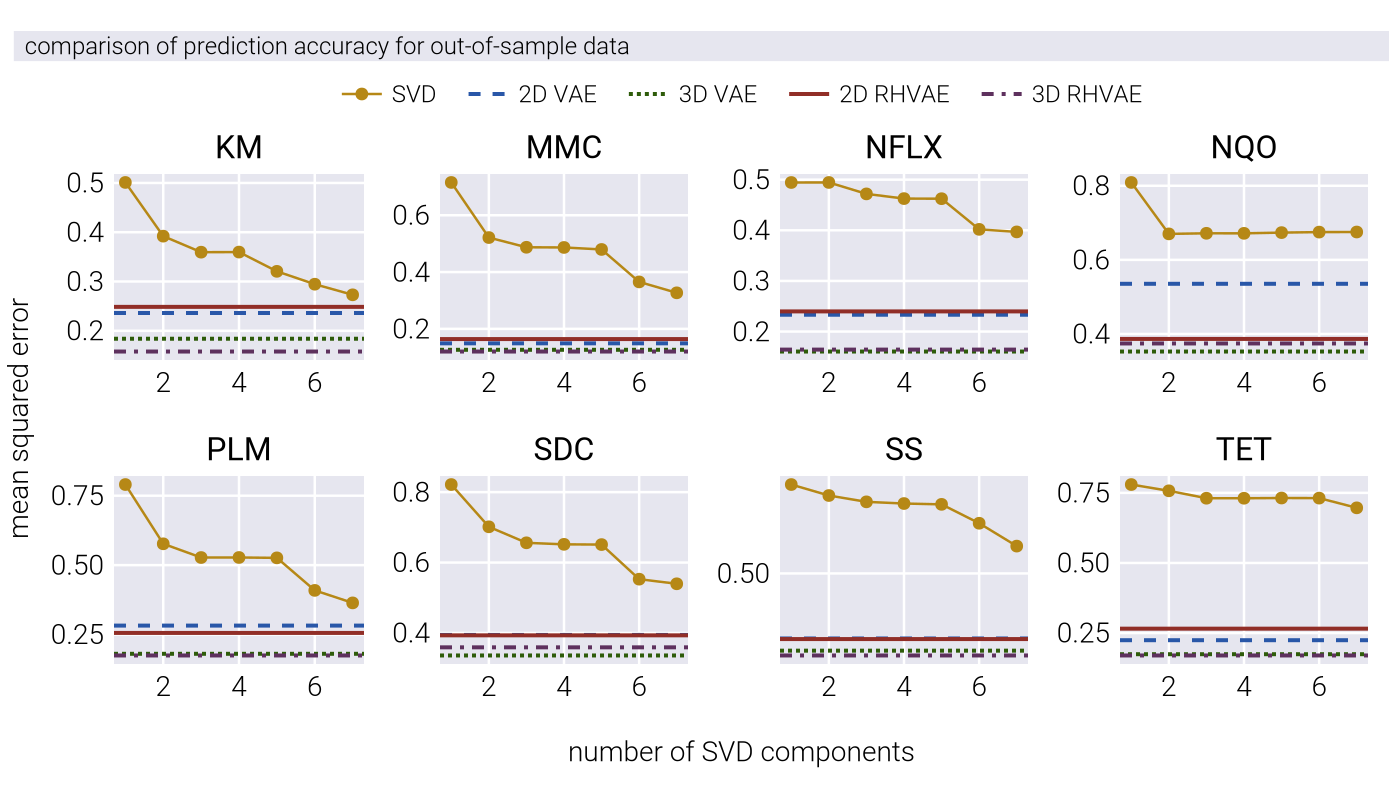
\includegraphics[keepaspectratio]{./fig/supplementary/figSI_data_2D-3D-crossval.pdf}}

}

\caption{\label{fig-SI-data-2D-3D-crossval}\textbf{Comparison of 2D and
3D nonlinear latent space models for predicting out-of-sample antibiotic
data}. Reconstruction error for each missing antibiotic as a function of
linear dimensions used in SVD cross-validation. Horizontal lines
represent the accuracy of nonlinear models: 2D-VAE (dark blue, dashed),
2D-RHVAE (dark red, solid), 3D-VAE (dark green, dotted), and 3D-RHVAE
(dark purple, dash-dotted). The 3D models show marginal improvement over
their 2D counterparts for most antibiotics, suggesting that two
effective degrees of freedom capture most of the relevant phenotypic
variation.}

\end{figure}%

\subsection{Geodesics in Latent Space}\label{geodesics-in-latent-space}

In this section, we explore an interesting and surprising property of
some of the resulting evolutionary trajectories in latent space. As
detailed in the main text, we trained an RHVAE on the \(IC_{50}\) data
from \autocite{iwasawa2022}. The data used to train the RHVAE consists
of a matrix with eight rows---one per each antibiotic---and \(\approx\)
1300 columns representing one of the lineages at some time point in the
experiment. However, at no point, the RHVAE has any knowledge of what
genotype or time point corresponds to any particular column in the data
matrix. All it sees at every epoch is a random subset of columns of this
matrix. Nevertheless, it is interesting to ask whether there is some
regularity in the resulting evolutionary trajectories in the learned
latent space. In other words, once the RHVAE is trained, we can map the
time series corresponding to a particular lineage to the corresponding
latent space trajectory. A few of these trajectories are shown in
Figure~\ref{fig-data-geodesics} as gold connected points.

One of the unique features of the RHVAE model is the co-learning of the
metric tensor in the latent space. A space endowed with such
mathematical structure gives us the ability to compute the shortest path
between any two points, commonly referred to as a geodesic. Geodesics
are the generalization of the idea of a straight line in Euclidean space
to curved spaces, and it is a fundamental concept in Riemannian
geometry. Let us define this curve as \(\underline{\gamma}(t)\) where
\(t \in [0, 1]\). This means that the geodesic is a parametric curve
\(\underline{\gamma}\) for which we only need to define the initial and
final points of the curve, \(\underline{\gamma}(0) = \underline{z}_0\)
and \(\underline{\gamma}(1) = \underline{z}_1\). What makes it a
geodesic is that it minimizes the length of the curve connecting the
initial and final points, i.e., it minimizes

\begin{equation}\phantomsection\label{eq-geodesic}{
L(\underline{\gamma}) = \int_0^1 
dt \,
\sqrt{
    \underline{\dot{\gamma}}(t)^T 
    \underline{\underline{G}}(\underline{\gamma}(t))
    \underline{\dot{\gamma}}(t)
}
}\end{equation}

where
\(\underline{\dot{\gamma}}(t) = \frac{d}{dt} \underline{\gamma}(t)\) is
the velocity vector of the curve and
\(\underline{\underline{G}}(\underline{\gamma}(t))\) is the metric
tensor at the point \(\underline{\gamma}(t)\). Computing this geodesic
is a non-trivial task, especially for a data-derived metric tensor with
no closed-form expression. Fortunately, we can leverage the generality
of neural networks to parameterize the curve and compute the geodesic
numerically \autocite{chen2018a}. Again, all we need to do is define the
initial and final points of the curve, provide the metric tensor learned
by the RHVAE, and let the neural network approximate the shortest path
between the two points. Figure~\ref{fig-data-geodesics} shows the
corresponding curves between the initial point (black crosses) and the
final point (black triangles) as red curves for a few lineages. We
highlight the fact that the curves are not straight lines in the latent
space, but rather curved paths that follow the curvature of the latent
space. For these few examples, we see that the geodesic curves are very
similar to the gold curves, which are the actual trajectories of the
lineages in the latent space. This rather surprising result suggests
that the best spatial representation for the evolutionary trajectories
coincides with the shortest path in the latent space.

\begin{figure}

\centering{

\pandocbounded{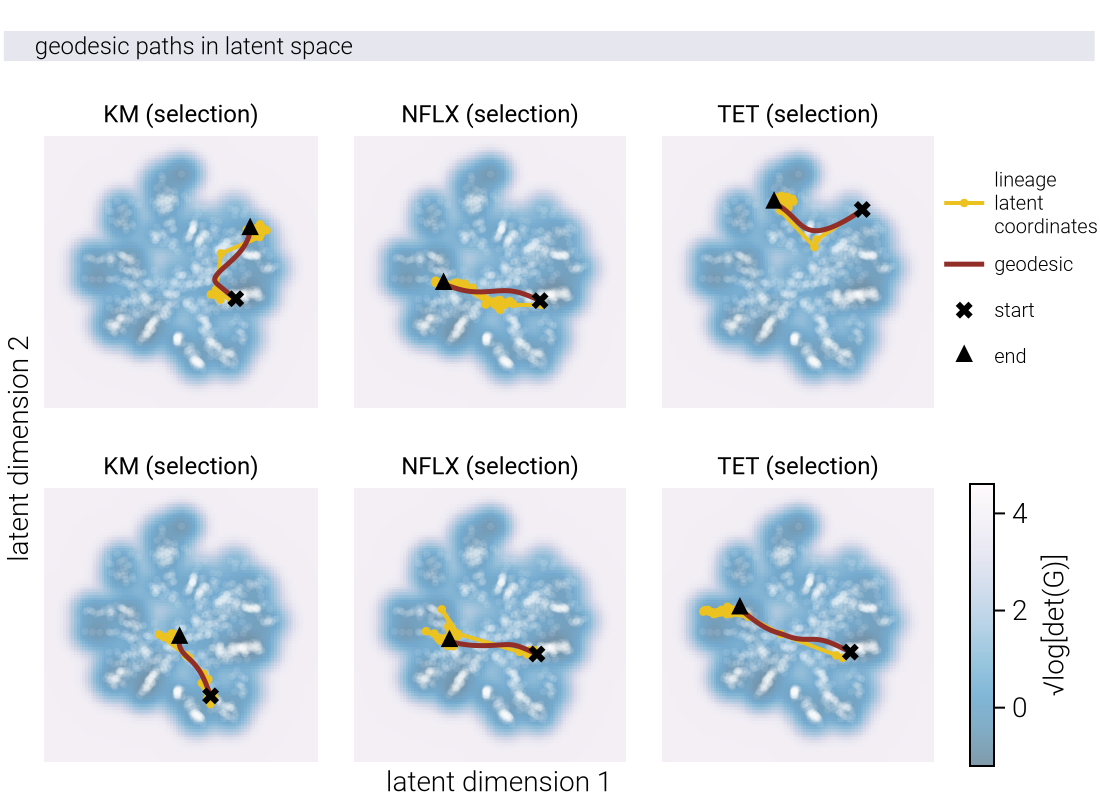
\includegraphics[keepaspectratio]{./fig/supplementary/figSI_data_geodesics.pdf}}

}

\caption{\label{fig-data-geodesics}\textbf{Geodesic paths in latent
space follow evolutionary trajectories} The figure shows the latent
space representation of evolutionary trajectories from the Iwasawa et
al.~dataset \autocite{iwasawa2022}. Background coloring represents the
metric volume (determinant of the metric tensor), with lighter regions
indicating higher local curvature. Gold connected points show actual
evolutionary trajectories of different lineages, while red curves
represent the computed geodesics (shortest paths) between initial points
(black crosses) and final points (black triangles). The striking
similarity between geodesics and actual trajectories suggests that
evolution in phenotype space tends to follow paths that minimize
distance in the geometry-informed latent space.}

\end{figure}%

So far, these few examples suggest that the shortest path in the latent
space coincides with the actual evolutionary trajectory. Since the
latent space coordinates of any data point capture information about the
resistance profile of the corresponding strain, we expect that the
qualitative matching between the geodesic and the actual trajectory
should mean that the resulting resistance profile predicted by the
geodesic is very similar to the actual experimental resistance profile.
To see if this is the case, we must decode the latent space trajectory
back to the original space. Doing so projects back all of the points
sampled along the geodesic curve to the original data space with eight
antibiotic resistance values. However, there is a catch: the geodesic
curve is a smooth continuous function of time, but the resistance
profile of a strain is a discrete set of values with different step
sizes. In other words, when constructing the geodesic curve, we define a
continuous function connecting the initial and final point with no
sudden jumps in the coordinates. But there is no \emph{a priori} reason
that the resulting experimental curve should be smooth. This statement
is not necessarily a consequence of the discrete sampling of the data
with a one-day time step that could be resolved by increasing the
sampling frequency, but rather a consequence of the genotype-phenotype
map. Although in the simulations presented in the main text we assume
that all evolutionary steps follow certain distribution of step sizes as
a convenient mathematical simplification, the complexity of the
genotype-phenotype map might be such that this simplification is not
valid. To emphasize this point even further, we can think of the
geodesic curve as a prediction of what the cross-resistance values for
the different antibiotics ought to be without information about when
those values must evolve in time.

The consequence of this is that it is not clear how to align the
continuous geodesic curve with the discrete experimental data. We can,
however, make use of methodologies developed for similar purposes in the
form of time-warping algorithms. In this case, we can use dynamic time
warping (DTW) to align the continuous geodesic curve with the discrete
experimental data. DTW is a well-known algorithm in the signal
processing community for aligning two time series with different step
sizes. Effectively, DTW finds the optimal pairing of points between the
two time series, with the constraint that the alignment is monotonic,
i.e., if point \(x_i\) in one time series is aligned to point \(y_j\) in
the other time series, then \(x_{i+1}\) is either aligned to \(y_{j}\)
or \(y_{j+1}\), never stepping backwards. We use this algorithm to align
the points sampled along the geodesic curve in latent space with the
resulting experimental curve also in latent space. This point, although
subtle, is important: the alignment is done in latent space, not in the
original data space. This means that the alignment is done based on the
metric tensor learned by the RHVAE, and not on the original data.

Once we have the aligned latent space trajectory, we can decode it back
to the original data space and plot the resulting experimental curve.
Figure~\ref{fig-data-geodesics-timewarp-1} and
Figure~\ref{fig-data-geodesics-timewarp-2} show the results of this
procedure for the same few lineages shown in
Figure~\ref{fig-data-geodesics}. On the left, we show the same latent
space trajectory as in Figure~\ref{fig-data-geodesics}, on the right, we
show the resulting \(IC_{50}\) curves for each of the eight antibiotics.
The gold curves show the original experimental curves, while the red
curves show the geodesic-predicted curves after the dynamic time warping
alignment. Although far from perfect, the alignment is remarkably good
considering that the predictions were drawn from only knowing the
initial and final points of the trajectory in latent space and then
computing the shortest path between them. This surprising result begs
for further experimental investigation along with extensive theoretical
analysis of why this phenomenon occurs. One tantalizing, although highly
speculative, possibility is that evolution proceeds in phenotype space
following a least action principle, i.e., the path taken by the
evolutionary trajectory is the one that minimizes the distance traveled
in phenotype space subject to the constraints of phenotype
accessibility, as modeled by our genotype-phenotype density function in
the main text.

\begin{figure}

\centering{

\pandocbounded{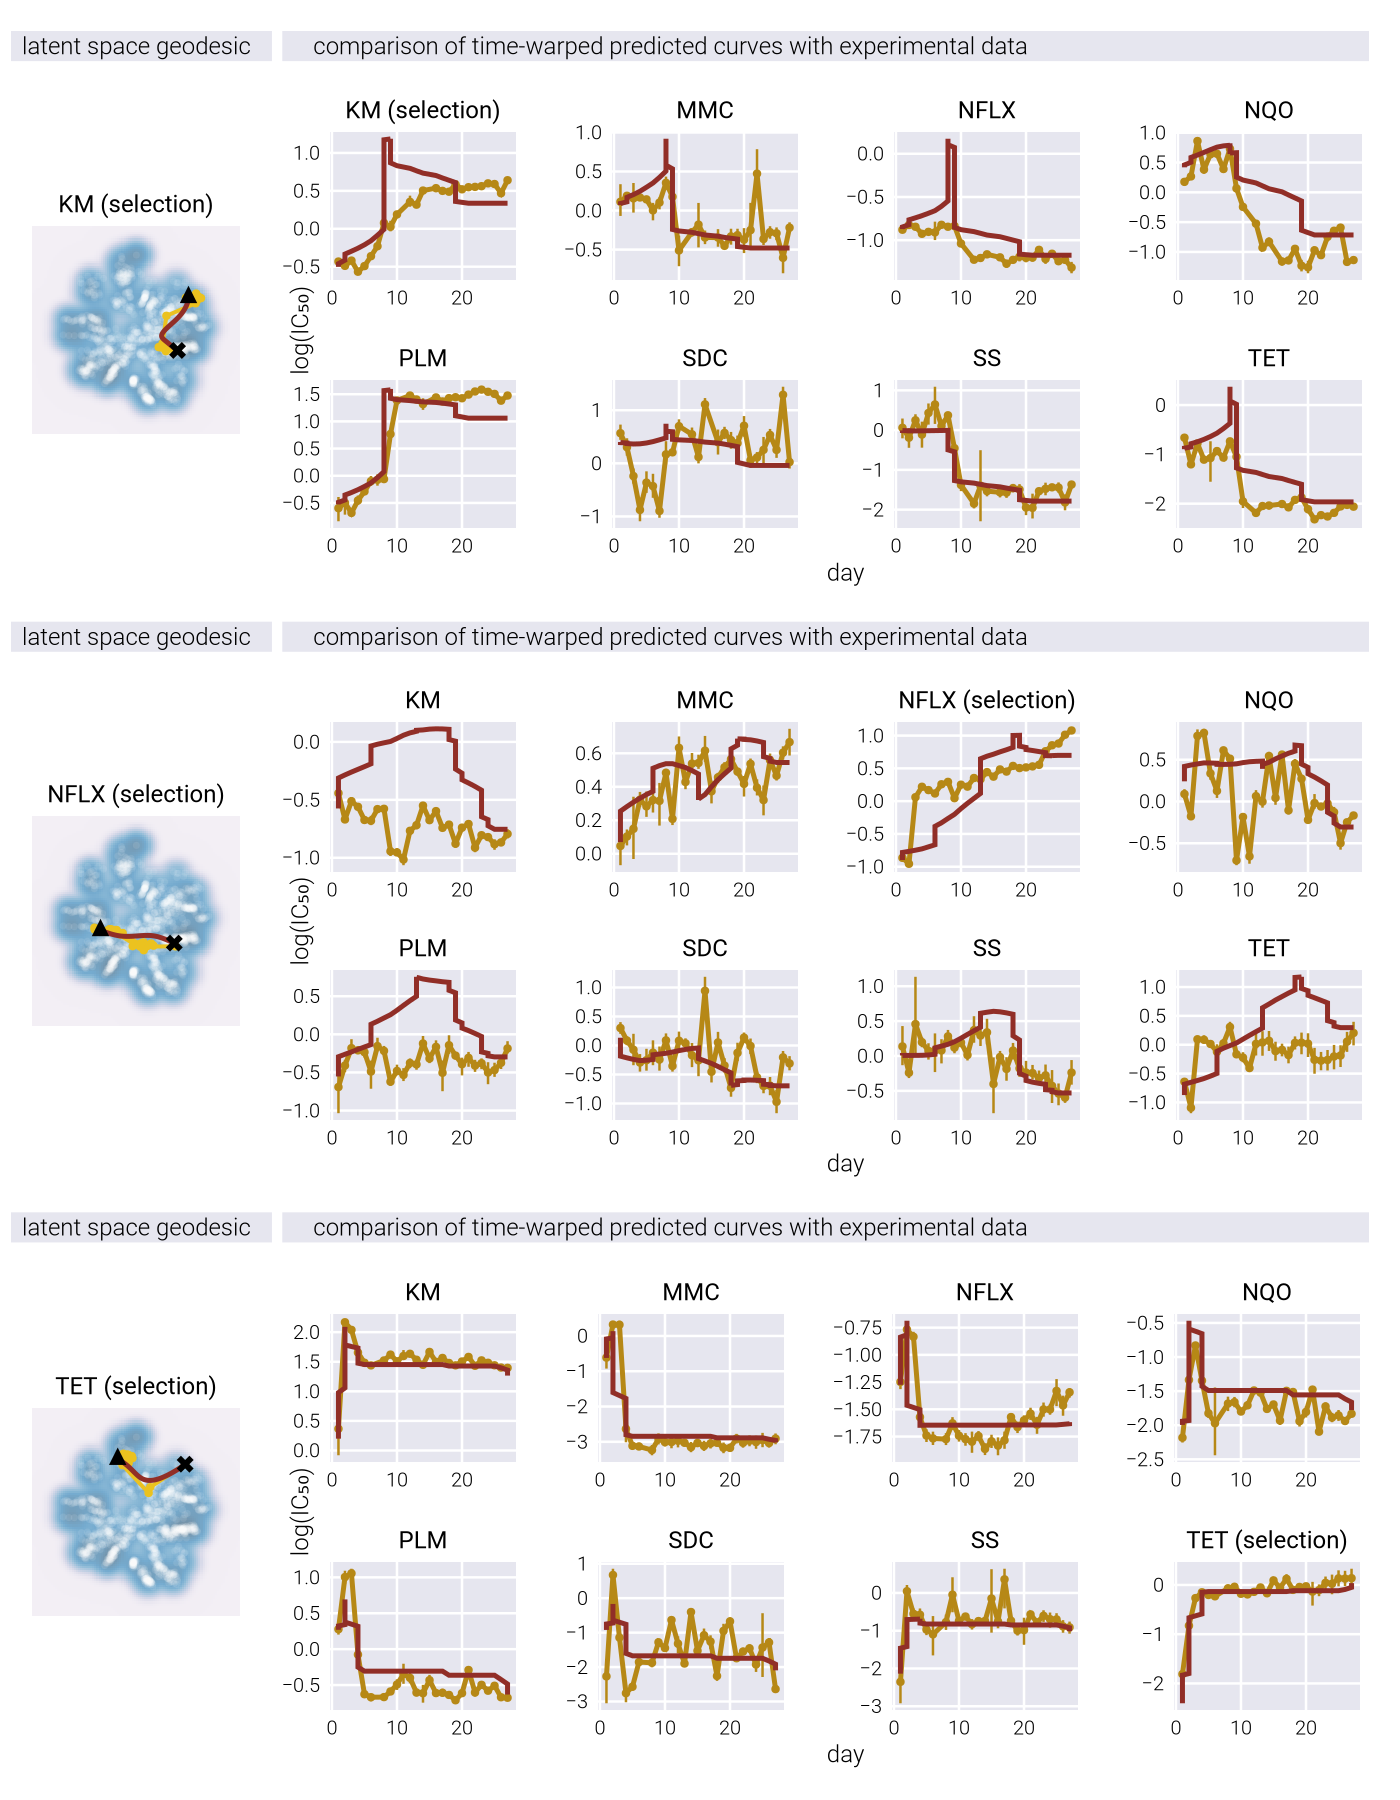
\includegraphics[keepaspectratio]{./fig/supplementary/figSI_data_geodesics_timewarp_1.pdf}}

}

\caption{\label{fig-data-geodesics-timewarp-1}\textbf{Geodesic
predictions of evolutionary trajectories match experimental data after
time alignment.} Left panel shows latent space trajectories (gold:
experimental path; red: geodesic prediction) for selected lineages.
Right panel shows the corresponding IC50 values for all eight
antibiotics over time, comparing experimental measurements (gold) with
geodesic predictions after dynamic time warping alignment (red).}

\end{figure}%

\begin{figure}

\centering{

\pandocbounded{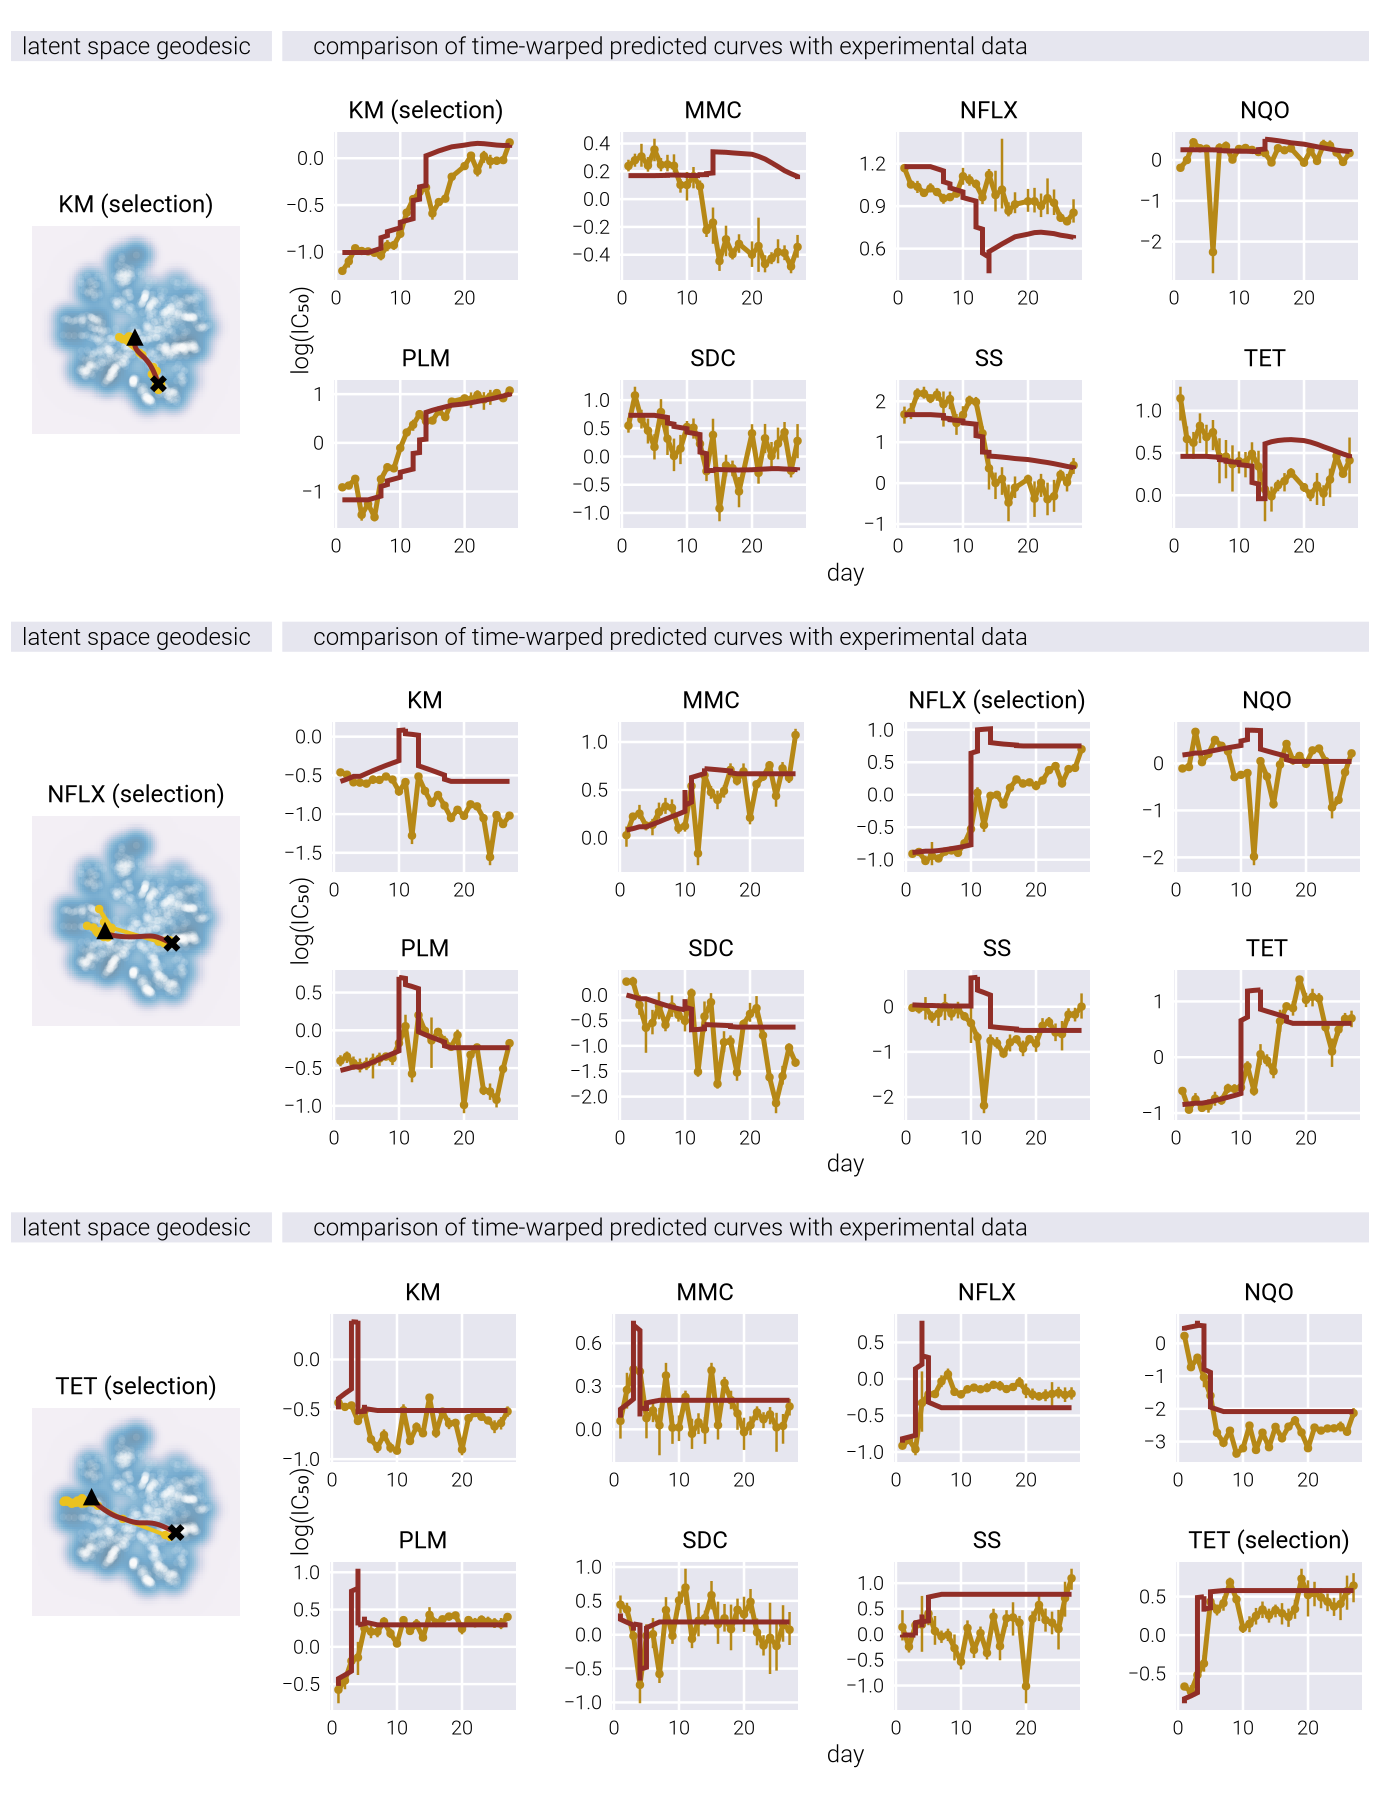
\includegraphics[keepaspectratio]{./fig/supplementary/figSI_data_geodesics_timewarp_2.pdf}}

}

\caption{\label{fig-data-geodesics-timewarp-2}\textbf{Additional
examples of geodesic-based predictions of antibiotic resistance
evolution.} Each panel pair shows another set of lineages where geodesic
paths in latent space (left, red curves) were used to predict the
temporal evolution of resistance profiles (right). Despite only using
initial and final points as inputs, the geodesic predictions (red)
capture many features of the actual evolutionary trajectories (gold)
after time alignment.}

\end{figure}%

\subsection{Geometry-Informed Latent Space Reconstruction of Antibiotic
Resistance
Landscapes}\label{geometry-informed-latent-space-reconstruction-of-antibiotic-resistance-landscapes}

In the main text, Figure 5 shows the ability of the RHVAE to reconstruct
the underlying fitness landscapes' topography from simulated data.
There, we demonstrated that the relative position, number of peaks, and
overall shape of the fitness landscapes are well-reproduced by the RHVAE
latent space. It is therefore interesting to show the same
reconstructions using the experimental data from \autocite{iwasawa2022}.

After training an RHVAE model on the \(IC_{50}\) data from
\autocite{iwasawa2022}---the same model used in the main text in Figure
6---we apply the same methodology to reconstruct the fitness landscapes
for the eight antibiotics used in the experiment.
Figure~\ref{fig-iwasawa-landscapes} shows the reconstructed fitness
landscapes for all eight antibiotics along with the latent space metric
volume. One obvious difference between the landscapes reconstructed from
the simulated and experimental data is the lack of clear peaks in the
experimental landscapes. Although it is possible that such peaks do not
exist, it is more likely that the lack of peaks is due to the limited
resolution of the experimental data, where only a few initial genotypes
were measured.

\begin{figure}

\centering{

\pandocbounded{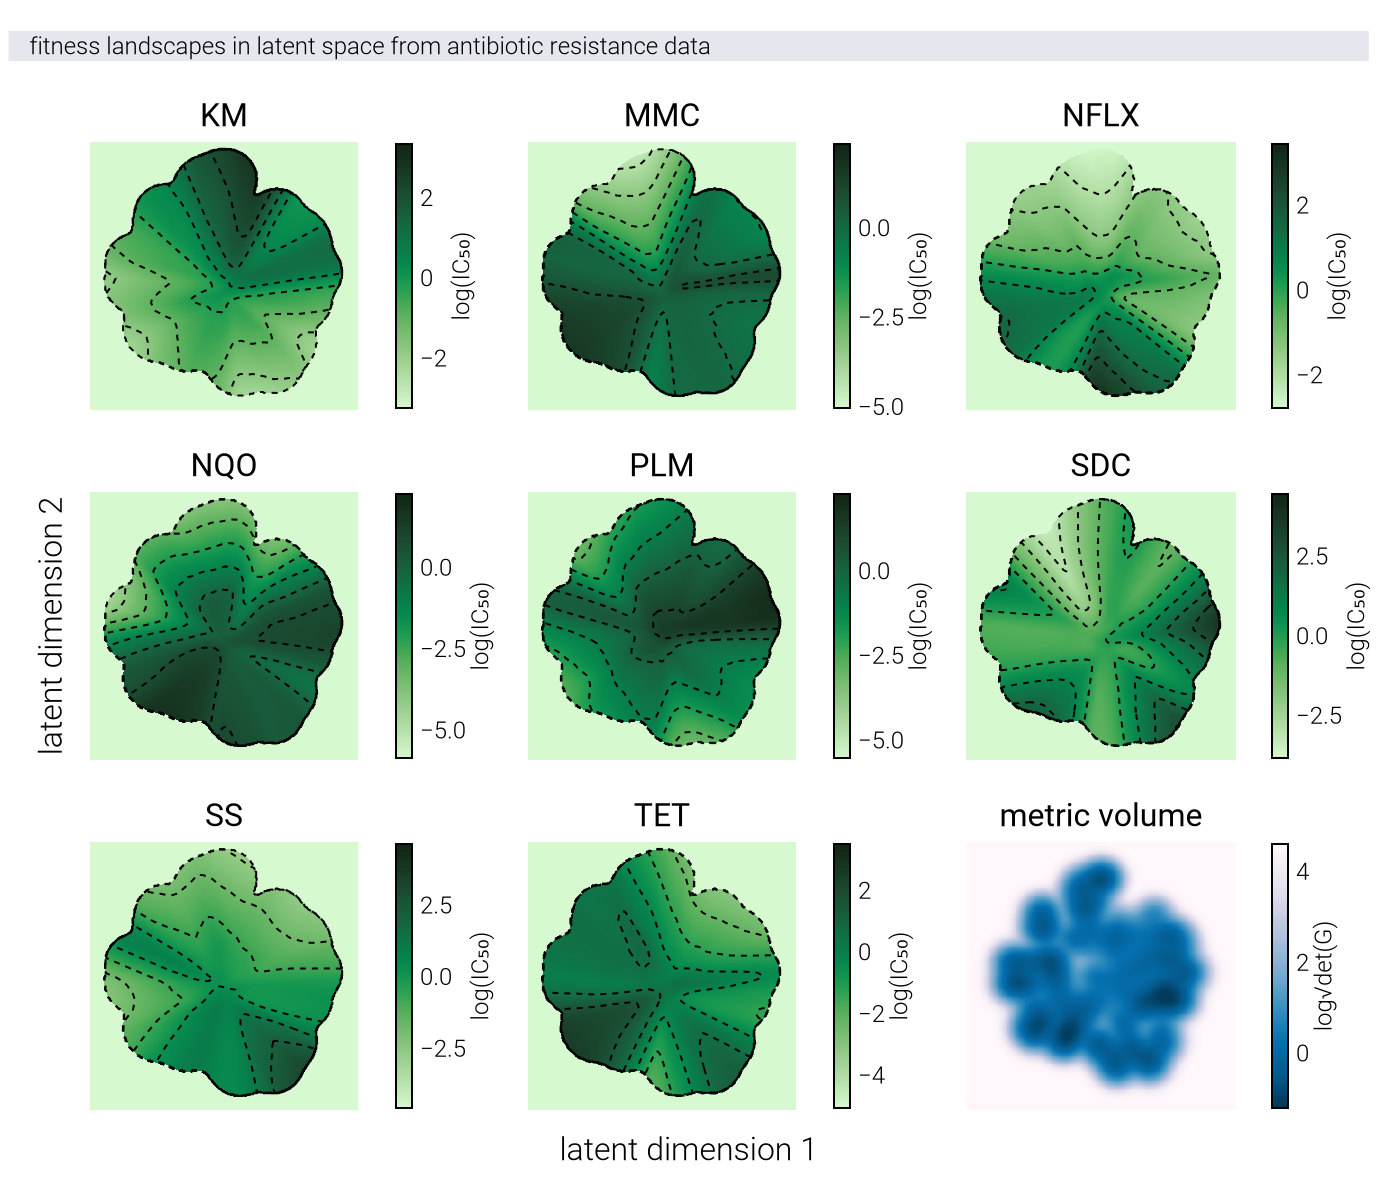
\includegraphics[keepaspectratio]{./fig/supplementary/figSI_iwasawa_landscapes.pdf}}

}

\caption{\label{fig-iwasawa-landscapes}\textbf{Reconstructed 2D
antibiotic resistance landscapes from experimental data}. The first
eight panels show the antibiotic resistance landscape reconstructions
using a 2D RHVAE trained on the \(IC_{50}\) data from
\autocite{iwasawa2022}. Dotted lines show different level curves on the
fitness landscape. The last panel shows the metric volume (the
determinant of the metric tensor) of the latent space. The darker the
color, the flatter the latent space.}

\end{figure}%

Given the lack of regularity in the resulting landscapes, we also show
the three-dimensional representations of the resistance landscapes for
different antibiotics using experimental data from
\autocite{iwasawa2022}. Figure~\ref{fig-iwasawa-3D-landscapes} shows the
same landscapes as in Figure~\ref{fig-iwasawa-landscapes}, but using the
z-axis to represent the fitness value. From this 3D perspective, the
lack of clear peaks is more apparent.

\begin{figure}

\centering{

\pandocbounded{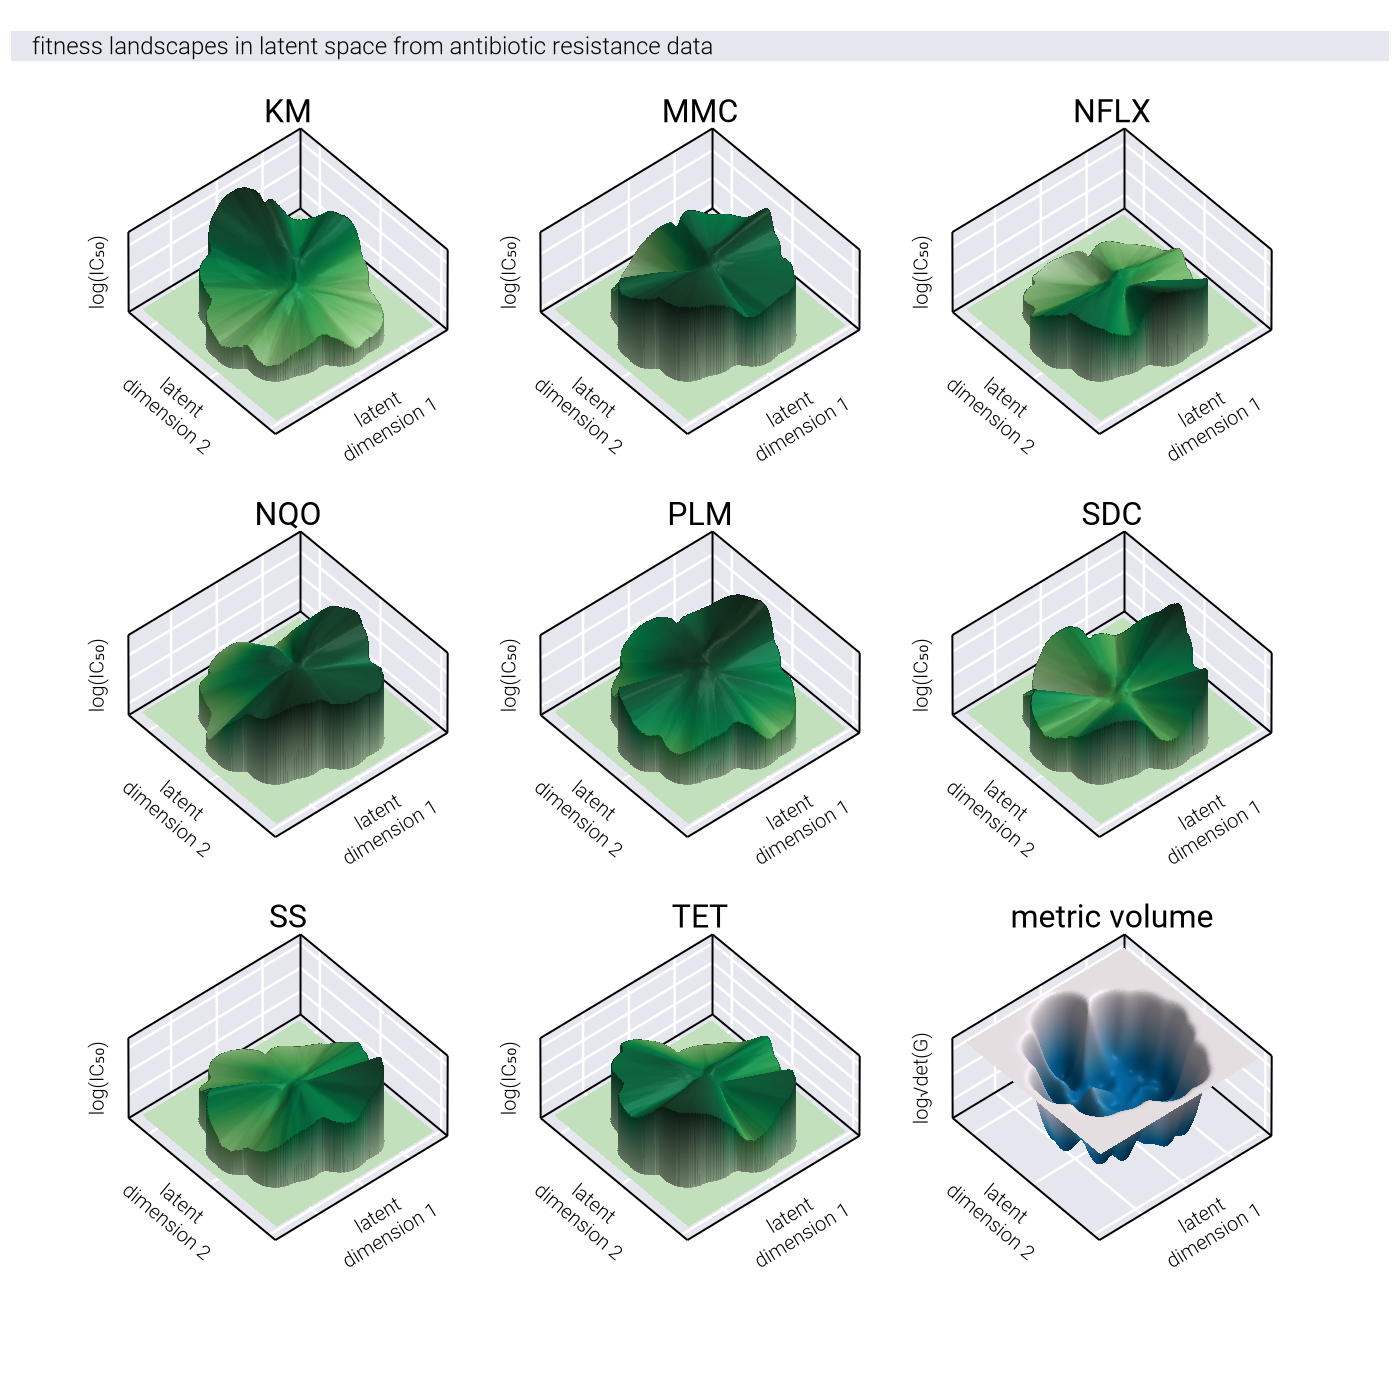
\includegraphics[keepaspectratio]{./fig/supplementary/figSI_iwasawa_3Dlandscapes.pdf}}

}

\caption{\label{fig-iwasawa-3D-landscapes}\textbf{3D visualization of
reconstructed antibiotic resistance landscapes}. Three-dimensional
representations of the same resistance landscapes shown in
Figure~\ref{fig-iwasawa-landscapes}, using experimental data from
\autocite{iwasawa2022}. The z-axis represents the fitness value (IC₅₀).
This 3D perspective more clearly illustrates the lack of distinct peaks
in the experimental data, which may be due to limited sampling of
initial genotypes rather than the absence of such features in the actual
fitness landscapes.}

\end{figure}%

\subsubsection{Trajectories in Experimentally-reconstructed Fitness
Landscapes}\label{trajectories-in-experimentally-reconstructed-fitness-landscapes}

Given these reconstructed fitness landscapes, we can now explore the
evolutionary trajectories of different lineages in the experimental
data. In \autocite{iwasawa2022}, the authors evolved genotypes in the
presence of three different antibiotics: \emph{Tetracycline} (TET),
\emph{Kanamycin} (KAN), and \emph{Norfloxacin} (NFLX). Naively, if these
fitness landscapes are representative of the underlying landscape
available to the genotypes, we would expect the trajectories of these
lineages to follow a noisy gradient ascent-like path in the latent
space, following the fitness gradient predicted by the reconstructed
landscapes. Figure~\ref{fig-iwasawa-trajectories-KM},
Figure~\ref{fig-iwasawa-trajectories-TET}, and
Figure~\ref{fig-iwasawa-trajectories-NFLX} show the evolutionary
trajectories of the lineages evolved in the presence of
\emph{Kanamycin}, \emph{Tetracycline}, and \emph{Norfloxacin},
respectively. The left and right panels show the same trajectories in
the 2D and 3D projection of the latent space, respectively. One of the
problematic aspects of these trajectories is that in none of the cases
do the trajectories follow a path towards the predicted highest fitness
peak. We strongly suspect this is a problem with the experimental setup,
rather than the entirety of our approach. Our suspicion is that the
selection of initial genotypes completely biased the reconstruction of
the fitness landscapes. Some of the lineages selected by the authors
were previously evolved in the presence of one of these antibiotics, to
then be re-evolved in the presence of the other antibiotics. In other
words, there were some strains in the initial pool that were already
highly resistant to, say, \emph{Kanamycin}, and then these strains were
re-evolved in the presence of \emph{Tetracycline}. The presence of these
strains explains the existence of those peaks that none of the
trajectories reach, since these strains evolved for much longer in the
corresponding antibiotic compared to this experimental setup. However,
further investigation is needed to determine the cause of this behavior.

\begin{figure}

\centering{

\pandocbounded{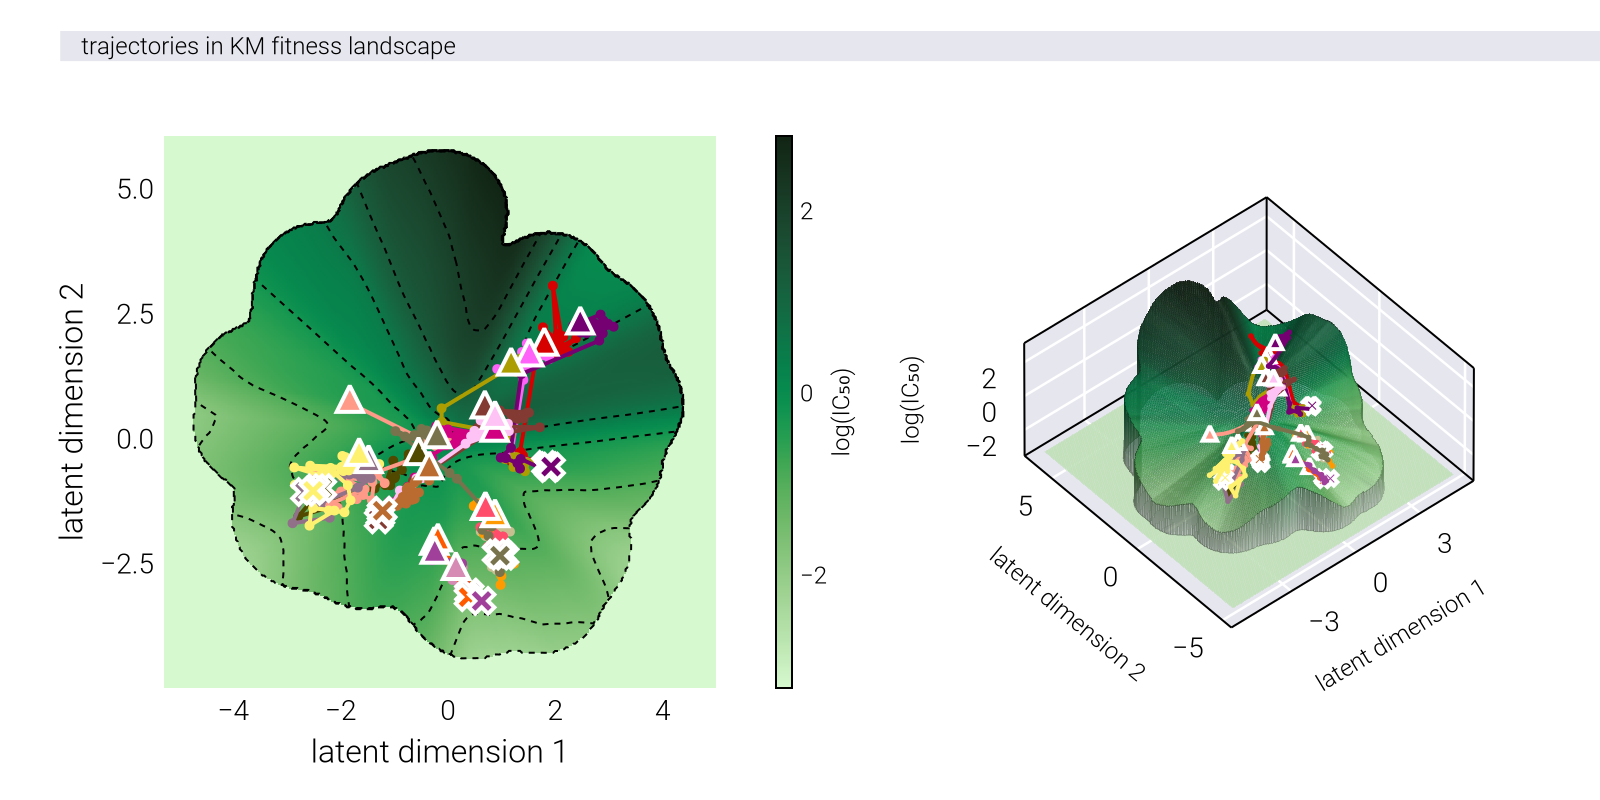
\includegraphics[keepaspectratio]{./fig/supplementary/figSI_iwasawa_landscapes_trajectories_KM.pdf}}

}

\caption{\label{fig-iwasawa-trajectories-KM}\textbf{Evolutionary
trajectories of lineages evolved in Kanamycin}. The left panel shows the
2D projection of evolutionary trajectories in the latent space overlaid
on the Kanamycin resistance landscape. The right panel shows the same
trajectories in a 3D projection. Different colors represent different
lineages. Cross symbols indicate the initial point of the trajectory,
while triangles indicate the final point. Note that trajectories do not
follow paths toward the highest predicted fitness peaks, suggesting
potential biases in the experimental setup or limitations in landscape
reconstruction.}

\end{figure}%

\begin{figure}

\centering{

\pandocbounded{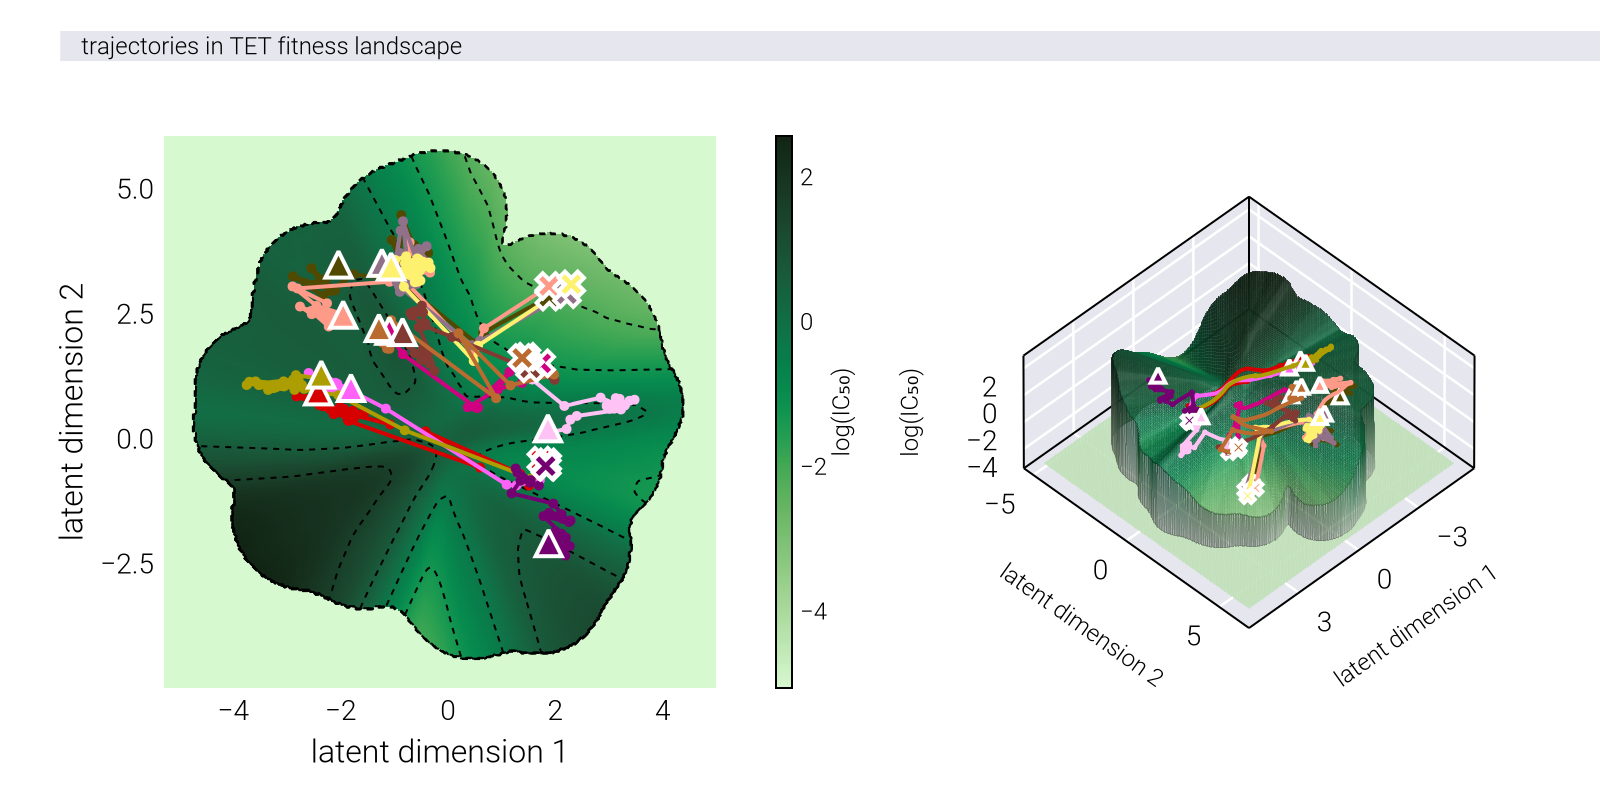
\includegraphics[keepaspectratio]{./fig/supplementary/figSI_iwasawa_landscapes_trajectories_TET.pdf}}

}

\caption{\label{fig-iwasawa-trajectories-TET}\textbf{Evolutionary
trajectories of lineages evolved in Tetracycline}. The left panel shows
the 2D projection of evolutionary trajectories in the latent space
overlaid on the Tetracycline resistance landscape. The right panel shows
the same trajectories in a 3D projection. Different colors represent
different lineages. Cross symbols indicate the initial point of the
trajectory, while triangles indicate the final point. Similar to the
Kanamycin case, trajectories do not consistently follow gradient ascent
paths toward fitness peaks.}

\end{figure}%

\begin{figure}

\centering{

\pandocbounded{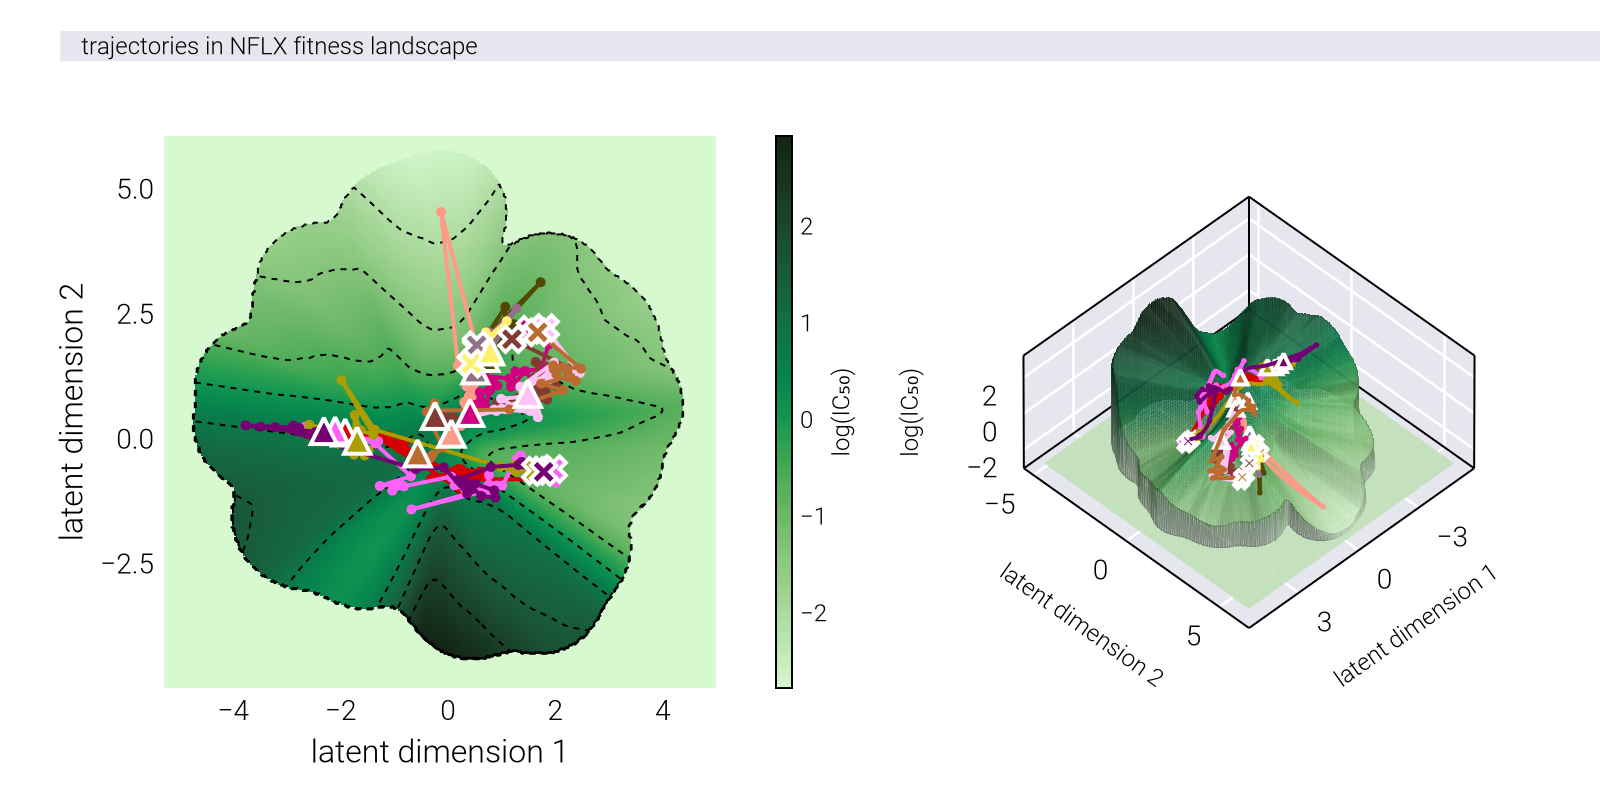
\includegraphics[keepaspectratio]{./fig/supplementary/figSI_iwasawa_landscapes_trajectories_NFLX.pdf}}

}

\caption{\label{fig-iwasawa-trajectories-NFLX}\textbf{Evolutionary
trajectories of lineages evolved in Norfloxacin}. The left panel shows
the 2D projection of evolutionary trajectories in the latent space
overlaid on the Norfloxacin resistance landscape. The right panel shows
the same trajectories in a 3D projection. Different colors represent
different lineages. Cross symbols indicate the initial point of the
trajectory, while triangles indicate the final point. As with other
antibiotics, the evolutionary paths do not align with the predicted
fitness gradients, potentially due to pre-evolved strains in the initial
pool biasing landscape reconstruction.}

\end{figure}%

\subsection{Neural Network
Architecture}\label{neural-network-architecture}

\subsubsection{RHVAE Overview}\label{rhvae-overview}

The neural network architecture implemented in this study is a
Riemannian Hamiltonian Variational Autoencoder (RHVAE)
\autocite{chadebec2020}. The network was implemented using the
\texttt{Flux.jl} framework \autocite{innes2018} via the
\texttt{AutoEncoderToolkit.jl} package \autocite{razo-mejia2024}, and
consists of three main components: an encoder, a decoder, and a metric
chain network for the Riemannian metric computations.

\subsubsection{Model Parameters}\label{model-parameters}

\begin{longtable}[]{@{}
  >{\raggedright\arraybackslash}p{(\linewidth - 4\tabcolsep) * \real{0.2568}}
  >{\raggedright\arraybackslash}p{(\linewidth - 4\tabcolsep) * \real{0.0676}}
  >{\raggedright\arraybackslash}p{(\linewidth - 4\tabcolsep) * \real{0.6757}}@{}}
\toprule\noalign{}
\begin{minipage}[b]{\linewidth}\raggedright
Parameter
\end{minipage} & \begin{minipage}[b]{\linewidth}\raggedright
Value
\end{minipage} & \begin{minipage}[b]{\linewidth}\raggedright
Description
\end{minipage} \\
\midrule\noalign{}
\endhead
\bottomrule\noalign{}
\endlastfoot
Latent Dimensions & 2 & Dimensionality of the latent space \\
Hidden Layer Size & 128 & Number of neurons in hidden layers \\
Temperature (T) & 0.8 & Temperature parameter for RHVAE \\
Regularization (λ) & 0.01 & Regularization parameter \\
Number of Centroids & 256 & Number of centroids for the manifold
approximation \\
\end{longtable}

\subsubsection{Encoder Architecture}\label{encoder-architecture}

The encoder implements a joint Gaussian log-encoder with the following
structure:

\begin{longtable}[]{@{}lll@{}}
\toprule\noalign{}
Layer & Output Dimensions & Activation Function \\
\midrule\noalign{}
\endhead
\bottomrule\noalign{}
\endlastfoot
Input & \texttt{n\_env}\(^*\) & - \\
Dense 1 & 128 & Identity \\
Dense 2 & 128 & LeakyReLU \\
Dense 3 & 128 & LeakyReLU \\
Dense 4 & 128 & LeakyReLU \\
µ output & 2 & Identity \\
logσ output & 2 & Identity \\
\end{longtable}

\(^*\) \texttt{n\_env} is the number of environments on which fitness is
determined to train the model.

\subsubsection{Decoder Architecture}\label{decoder-architecture}

The decoder implements a simple Gaussian decoder with the following
structure:

\begin{longtable}[]{@{}lll@{}}
\toprule\noalign{}
Layer & Output Dimensions & Activation Function \\
\midrule\noalign{}
\endhead
\bottomrule\noalign{}
\endlastfoot
Input & 2 & - \\
Dense 1 & 128 & Identity \\
Dense 2 & 128 & LeakyReLU \\
Dense 3 & 128 & LeakyReLU \\
Dense 4 & 128 & LeakyReLU \\
Output & \texttt{n\_env} & Identity \\
\end{longtable}

\subsubsection{Metric Chain
Architecture}\label{metric-chain-architecture}

The metric chain computes the Riemannian metric tensor with the
following structure:

\begin{longtable}[]{@{}lll@{}}
\toprule\noalign{}
Layer & Output Dimensions & Activation Function \\
\midrule\noalign{}
\endhead
\bottomrule\noalign{}
\endlastfoot
Input & \texttt{n\_env} & - \\
Dense 1 & 128 & Identity \\
Dense 2 & 128 & LeakyReLU \\
Dense 3 & 128 & LeakyReLU \\
Dense 4 & 128 & LeakyReLU \\
Diagonal Output & 2 & Identity \\
Lower Triangular Output & 1 & Identity \\
\end{longtable}

\subsubsection{Data Preprocessing}\label{data-preprocessing}

The input data underwent the following preprocessing steps:

\begin{enumerate}
\def\labelenumi{\arabic{enumi}.}
\item
  Logarithmic transformation of fitness values.
\item
  Z-score standardization (mean = 0, std = 1) per environment.
\item
  K-medoids clustering to select centroids for the manifold
  approximation.
\end{enumerate}

\subsubsection{Implementation Details}\label{implementation-details-1}

The model was implemented using:

\begin{itemize}
\item
  \texttt{Julia} programming language.
\item
  \texttt{Flux.jl} for neural network architecture.
\item
  \texttt{AutoEncoderToolkit.jl} for RHVAE-specific components.
\item
  Random seed set to 42 for reproducibility.
\end{itemize}

The complete model state and architecture were saved in \texttt{JLD2}
format for reproducibility and future use.

All of the code used to implement the model is available in the GitHub
repository for this project.

\subsection{Neural Geodesic
Architecture}\label{neural-geodesic-architecture}

The neural network architecture implemented in this study is a Neural
Geodesic model designed to find geodesics on the latent space manifold
of a Riemannian Hamiltonian Variational Autoencoder (RHVAE)
\autocite{chen2018a}. The network is implemented using the Flux.jl
framework and learns to parameterize geodesic curves between points in
the latent space.

\subsubsection{Model Parameters}\label{model-parameters-1}

\begin{longtable}[]{@{}
  >{\raggedright\arraybackslash}p{(\linewidth - 4\tabcolsep) * \real{0.2179}}
  >{\raggedright\arraybackslash}p{(\linewidth - 4\tabcolsep) * \real{0.3205}}
  >{\raggedright\arraybackslash}p{(\linewidth - 4\tabcolsep) * \real{0.4615}}@{}}
\toprule\noalign{}
\begin{minipage}[b]{\linewidth}\raggedright
Parameter
\end{minipage} & \begin{minipage}[b]{\linewidth}\raggedright
Value
\end{minipage} & \begin{minipage}[b]{\linewidth}\raggedright
Description
\end{minipage} \\
\midrule\noalign{}
\endhead
\bottomrule\noalign{}
\endlastfoot
Hidden Layer Size & 32 & Number of neurons in hidden layers \\
Input Dimension & 1 & Time parameter t ∈ {[}0,1{]} \\
Output Dimension & 2 & Dimensionality of the latent space \\
Endpoints & z\_init={[}0,0{]}, z\_end={[}1,1{]} & Start and end points
of the geodesic \\
\end{longtable}

\subsubsection{Neural Geodesic
Architecture}\label{neural-geodesic-architecture-1}

The neural geodesic implements a feed-forward network that maps from the
time domain to the latent space with the following structure:

\begin{longtable}[]{@{}lll@{}}
\toprule\noalign{}
Layer & Output Dimensions & Activation Function \\
\midrule\noalign{}
\endhead
\bottomrule\noalign{}
\endlastfoot
Input & 1 & - \\
Dense 1 & 32 & Identity \\
Dense 2 & 32 & TanH \\
Dense 3 & 32 & TanH \\
Dense 4 & 32 & TanH \\
Output & 2 & Identity \\
\end{longtable}

\subsubsection{Architectural Details}\label{architectural-details}

\begin{enumerate}
\def\labelenumi{\arabic{enumi}.}
\tightlist
\item
  \textbf{Input Processing}

  \begin{itemize}
  \tightlist
  \item
    Takes a single time parameter \(t \in [0,1]\).
  \item
    Maps to the latent space dimension (2D in this implementation).
  \item
    Designed to learn smooth geodesic curves.
  \end{itemize}
\item
  \textbf{Network Structure}

  \begin{itemize}
  \tightlist
  \item
    Follows a deep architecture with 4 hidden layers.
  \item
    Uses \texttt{tanh} activation for smooth curve generation.
  \item
    Identity activation at input and output layers for unrestricted
    range.
  \end{itemize}
\item
  \textbf{Output Constraints}

  \begin{itemize}
  \tightlist
  \item
    Network outputs must satisfy boundary conditions:

    \begin{itemize}
    \tightlist
    \item
      \(\gamma(0) = \underline{z}_{\text{init}}\).
    \item
      \(\gamma(1) = \underline{z}_{\text{end}}\).
    \end{itemize}
  \item
    Generated curve represents path in latent space.
  \end{itemize}
\end{enumerate}

\subsubsection{Implementation Details}\label{implementation-details-2}

The model is implemented with:

\begin{itemize}
\item
  \texttt{Julia} programming language.
\item
  \texttt{Flux.jl} for neural network architecture.
\item
  \texttt{AutoEncode.diffgeo} package for geodesic-specific components.
\item
  Random seed set to 42 for reproducibility.
\end{itemize}

The model is designed to work in conjunction with a pre-trained RHVAE
model, using its latent space structure to inform the geodesic
computation. The complete model state and architecture are saved in
\texttt{JLD2} format for reproducibility and future use.

\subsubsection{Integration with RHVAE}\label{integration-with-rhvae}

This neural geodesic model complements the RHVAE architecture by:

\begin{enumerate}
\def\labelenumi{\arabic{enumi}.}
\item
  Using the same latent space dimensionality.
\item
  Learning geodesics that respect the Riemannian metric of the RHVAE
\item
  Providing a parameterized way to interpolate between latent points
\end{enumerate}

\subsection{Latent Space Alignment via Procrustes
Analysis}\label{latent-space-alignment-via-procrustes-analysis}

When working with different dimensionality reduction techniques such as
PCA, VAE, and RHVAE, the resulting latent spaces often have arbitrary
orientations that make direct comparisons challenging. To facilitate
meaningful comparisons between these latent representations and the
ground truth phenotype space, we employed Procrustes analysis. This
section details the mathematical foundations and implementation of our
alignment procedure.

\subsubsection{Mathematical Formulation}\label{mathematical-formulation}

Procrustes analysis finds an optimal rigid transformation (rotation,
scaling, and potentially translation) that aligns one set of points with
another while minimizing the sum of squared differences. Given two sets
of points \(\underline{\underline{X}}\) and
\(\underline{\underline{Y}}\), where each column represents a point in
\(\mathbb{R}^d\), the objective is to find a transformation of
\(\underline{\underline{X}}\) that best aligns with
\(\underline{\underline{Y}}\).

The Procrustes problem can be formulated as:

\begin{equation}\phantomsection\label{eq-procrustes}{
\min_{R, s} \|
    \underline{\underline{Y}} - 
    s\underline{\underline{X}}\,\underline{\underline{R}}
\|_F^2
}\end{equation}

where:

\begin{itemize}
\tightlist
\item
  \(\underline{\underline{R}}\) is a \(d \times d\) orthogonal rotation
  matrix (\(\underline{\underline{R}}^T\underline{\underline{R}} =
  \underline{\underline{I}}\))
\item
  \(s\) is a scalar scaling factor
\item
  \(\|\cdot\|_F\) denotes the Frobenius norm
\end{itemize}

If the data is centered (mean-subtracted), the transformation involves
only rotation and scaling. The solution to this optimization problem is
obtained through Singular Value Decomposition (SVD).

\subsubsection{Algorithmic Procedure}\label{algorithmic-procedure}

Our implementation of Procrustes analysis follows these steps:

\begin{enumerate}
\def\labelenumi{\arabic{enumi}.}
\tightlist
\item
  \textbf{Data Standardization}: Each latent representation (PCA, VAE,
  RHVAE) and the ground truth phenotype data are standardized to have
  zero mean and unit standard deviation along each dimension:
\end{enumerate}

\begin{equation}\phantomsection\label{eq-standardization}{
\hat{\underline{\underline{X}}} = 
\frac{
    \underline{\underline{X}} -
    \underline{\mu}_X
}{
    \underline{\sigma}_X
}
}\end{equation}

where \(\underline{\mu}_X\) and \(\underline{\sigma}_X\) are the mean
and standard deviation vectors computed across all points in the
respective space.

\begin{enumerate}
\def\labelenumi{\arabic{enumi}.}
\setcounter{enumi}{1}
\tightlist
\item
  \textbf{Inner Product Computation}: We compute the inner product
  matrix between the standardized ground truth phenotype data
  \(\hat{\underline{\underline{Y}}}\) and each standardized latent
  representation \(\hat{\underline{\underline{X}}}\):
\end{enumerate}

\begin{equation}\phantomsection\label{eq-inner-product}{
\underline{\underline{A}} = 
\hat{\underline{\underline{Y}}}\,
\hat{\underline{\underline{X}}}^T
}\end{equation}

\begin{enumerate}
\def\labelenumi{\arabic{enumi}.}
\setcounter{enumi}{2}
\tightlist
\item
  \textbf{Singular Value Decomposition}: We perform SVD on the inner
  product matrix:
\end{enumerate}

\begin{equation}\phantomsection\label{eq-svd}{
\underline{\underline{A}} = 
\underline{\underline{U}}\,
\underline{\underline{\Sigma}}\,
\underline{\underline{V}}^T
}\end{equation}

where \(\underline{\underline{U}}\) and \(\underline{\underline{V}}\)
are orthogonal matrices, and \(\underline{\underline{\Sigma}}\) is a
diagonal matrix of singular values.

\begin{enumerate}
\def\labelenumi{\arabic{enumi}.}
\setcounter{enumi}{3}
\tightlist
\item
  \textbf{Rotation Matrix Computation}: The optimal rotation matrix is
  given by:
\end{enumerate}

\begin{equation}\phantomsection\label{eq-rotation}{
\underline{\underline{R}} = 
\underline{\underline{U}}\,
\underline{\underline{V}}^T
}\end{equation}

\begin{enumerate}
\def\labelenumi{\arabic{enumi}.}
\setcounter{enumi}{4}
\tightlist
\item
  \textbf{Scaling Factor Computation}: The optimal scaling factor is
  calculated as:
\end{enumerate}

\begin{equation}\phantomsection\label{eq-scaling}{
s = \frac{
        \text{tr}(\underline{\underline{\Sigma}})
    }{
        \|\hat{\underline{\underline{X}}}\|_F^2
    }
}\end{equation}

where \(\text{tr}(\underline{\underline{\Sigma}})\) is the trace of
\(\underline{\underline{\Sigma}}\) (sum of singular values) and
\(\|\hat{\underline{\underline{X}}}\|_F^2\) is the squared Frobenius
norm of \(\hat{\underline{\underline{X}}}\).

\begin{enumerate}
\def\labelenumi{\arabic{enumi}.}
\setcounter{enumi}{5}
\tightlist
\item
  \textbf{Transformation Application}: Each latent representation is
  transformed using the corresponding rotation matrix:
\end{enumerate}

\begin{equation}\phantomsection\label{eq-alignment}{
\underline{\underline{X}}_{\text{aligned}} = 
\underline{\underline{R}}\,\hat{\underline{\underline{X}}}
}\end{equation}

\begin{enumerate}
\def\labelenumi{\arabic{enumi}.}
\setcounter{enumi}{6}
\tightlist
\item
  \textbf{Similarity Metric Calculation}: We compute a correlation-like
  measure to quantify the goodness-of-fit between the aligned spaces:
\end{enumerate}

\begin{equation}\phantomsection\label{eq-correlation}{
\rho = \frac{
    \text{tr}(\underline{\underline{\Sigma}})
}{
    \|\hat{\underline{\underline{X}}}\|_F\|\hat{\underline{\underline{Y}}}\|_F
}
}\end{equation}

This metric ranges from 0 (no similarity) to 1 (perfect alignment).

\subsubsection{Significance for Comparative
Analysis}\label{significance-for-comparative-analysis}

The Procrustes alignment enables several critical aspects of our
analysis:

\begin{enumerate}
\def\labelenumi{\arabic{enumi}.}
\item
  \textbf{Direct Visual Comparison}: By aligning all latent spaces to
  the same orientation as the ground truth phenotype space, we can
  directly visualize and compare the structural preservation properties
  of each dimensionality reduction technique.
\item
  \textbf{Quantitative Assessment}: The correlation metric \(\rho\)
  provides a quantitative measure of how well each latent representation
  preserves the geometric structure of the ground truth phenotype space.
\item
  \textbf{Geometric Structure Preservation}: The alignment allows us to
  assess how features such as local neighborhoods, relative distances,
  and global structure are preserved in each latent representation.
\item
  \textbf{Trajectory Analysis}: For evolutionary trajectories, the
  alignment enables comparison of path lengths, directional changes, and
  convergence patterns across different representations.
\end{enumerate}

This alignment procedure forms the foundation for the comparative
analysis presented in the main text, where we evaluate the effectiveness
of different dimensionality reduction techniques in capturing the
underlying structure of the phenotype space.

\subsection{Alternative Metropolis-Kimura Evolutionary
Dynamics}\label{sec-metropolis-kimura}

In the main text, we described a simple algorithm for evolving a
population as a biased random walk on a phenotypic space controlled by
both a fitness function and a genotype-phenotype density function. Here,
we propose an alternative algorithm that combines elements of the
Metropolis-Hastings algorithm with Kimura's classical population
genetics theory.

\subsubsection{Metropolis-Kimura
Algorithm}\label{metropolis-kimura-algorithm}

In Section~\ref{sec-metropolis}, we described a simple framework with a
fitness function and a genotype-phenotype density function. Here, we use
the same framework but introduce a biologically motivated algorithm for
the evolutionary dynamics that combines elements of the
Metropolis-Hastings algorithm with Kimura's classical population
genetics theory. This approach implements a two-step process that
separately models:

\begin{enumerate}
\def\labelenumi{\arabic{enumi}.}
\tightlist
\item
  The probability of mutation occurring (mutation accessibility) as
  governed by the genotype-phenotype density.
\item
  The probability of fixation within a population (selection) determined
  by the fitness effect of such mutation and the effective population
  size.
\end{enumerate}

\paragraph{Biological Motivation}\label{biological-motivation}

In natural populations, evolution proceeds through two distinct
processes:

\begin{enumerate}
\def\labelenumi{\arabic{enumi}.}
\item
  \textbf{Mutation}: New variants arise through random genetic changes.
  The probability of specific mutations depends on molecular mechanisms
  and constraints of the genotype-phenotype map.
\item
  \textbf{Fixation}: Once a mutation occurs, it must spread through the
  population to become fixed. The probability of fixation depends on the
  selection coefficient (fitness advantage) and the effective population
  size.
\end{enumerate}

\paragraph{Mathematical Framework}\label{mathematical-framework}

\subparagraph{Mutation Probability}\label{mutation-probability}

The probability of a mutation from phenotype \(\underline{x}\) to
\(\underline{x}'\) is modeled using a Metropolis-like criterion based on
the genotype-phenotype density:

\begin{equation}\phantomsection\label{eq-mutation-probability}{
\pi_{\text{mut}}(\underline{x} \to \underline{x}') = 
\min\left(1, \left(\frac{GP(\underline{x}')}{GP(\underline{x})}\right)^{\beta}\right)
}\end{equation}

Here, \(GP(\underline{x})\) represents the genotype-phenotype density at
phenotype \(\underline{x}\), and \(\beta\) is a parameter controlling
the strength of mutational constraints. The higher \(\beta\) is, the
less likely a mutation going downhill in genotype-phenotype density is
to be accepted.

\subparagraph{Kimura's Fixation
Probability}\label{kimuras-fixation-probability}

Once a mutation occurs, its probability of fixation in a population of
effective size \(N\) is given by Kimura's formula

\begin{equation}\phantomsection\label{eq-kimura-fixation-probability}{
\pi_{\text{fix}}(\underline{x} \to \underline{x}') = 
\frac{1 - e^{-2s}}{1 - e^{-2Ns}}
}\end{equation}

where \(s\) is the selection coefficient. We compute this selection
coefficient as the difference in fitness between the new and old
phenotype divided by the fitness of the old phenotype:

\begin{equation}\phantomsection\label{eq-selection-coefficient}{
s = \frac{F_E(\underline{x}') - F_E(\underline{x})}{F_E(\underline{x})}
}\end{equation}

This equation captures a fundamental result from population genetics:
beneficial mutations (\(s > 0\)) have a higher probability of fixation,
with the probability approaching \(2s\) for small positive selection
coefficients and approaching 1 for large positive selection
coefficients. Deleterious mutations (\(s < 0\)) have an exponentially
decreasing probability of fixation as population size increases.

\paragraph{Overall Acceptance
Probability}\label{overall-acceptance-probability}

The overall acceptance probability---defined as the probability of a
proposed step \(\underline{x} \rightarrow \underline{x}'\)---is the
product of the mutation probability and the fixation probability:

\begin{equation}\phantomsection\label{eq-overall-acceptance-probability}{
\pi_{\text{accept}}(\underline{x} \to \underline{x}') = 
\pi_{\text{mut}}(\underline{x} \to \underline{x}') \cdot 
\pi_{\text{fix}}(\underline{x} \to \underline{x}')
}\end{equation}

This two-step process better reflects the biological reality of
evolution, where both mutational accessibility and selection contribute
to evolutionary trajectories.

\subsubsection{Effect of Population
Size}\label{effect-of-population-size}

Figure~\ref{fig-metropolis-population-effect} shows the effect of
population size parameter \(N\) influences evolutionary trajectories in
our Metropolis-Kimura framework. Through a series of panels showing both
phenotypic trajectories (upper) and fitness dynamics (lower), we can
observe how different population sizes affect the balance between
exploration and exploitation in phenotypic space.

At small population sizes (left panels), the evolutionary trajectories
exhibit highly stochastic behavior, with populations taking meandering
paths through the phenotypic landscape. This represents a regime where
genetic drift plays a dominant role. As population size increases
(moving right), the trajectories become increasingly deterministic, with
populations taking more direct paths toward fitness peaks, while
avoiding genotype-to-phenotype density valleys. This transition reflects
a shift from drift-dominated to selection-dominated dynamics, where
populations more strictly follow the local fitness gradient. The fitness
trajectories in the lower panels further reinforce this pattern, showing
more erratic fitness fluctuations at small population sizes and more
monotonic increases at large population sizes, consistent with stronger
selective pressures.

\begin{figure}

\centering{

\pandocbounded{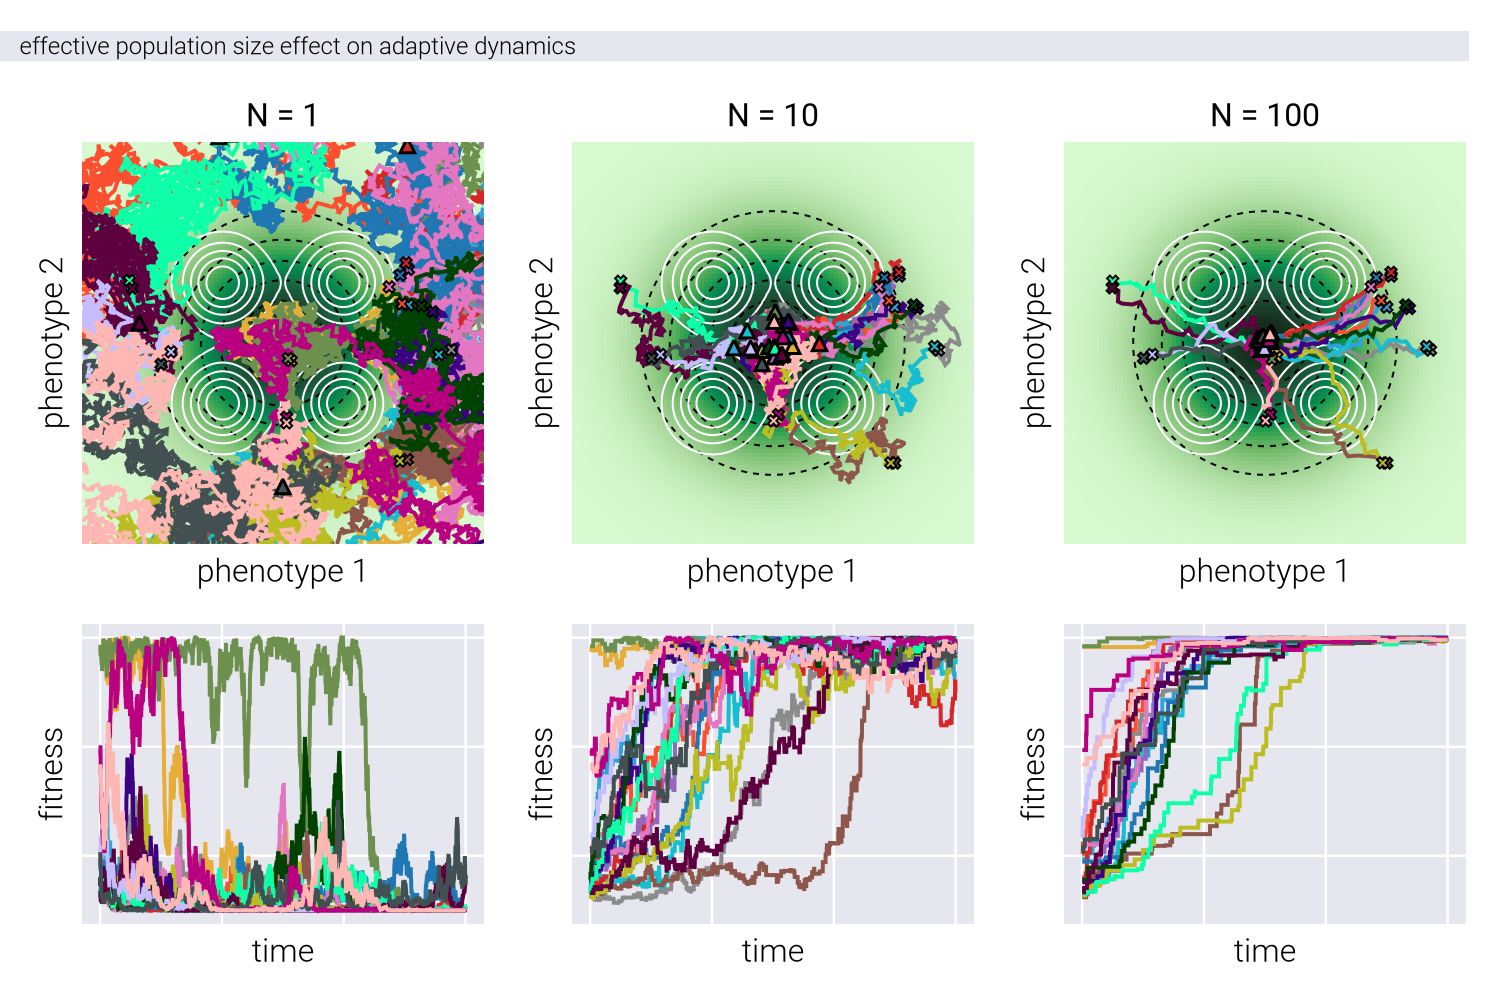
\includegraphics[keepaspectratio]{./fig/supplementary/figSI_sim_population_effect.pdf}}

}

\caption{\label{fig-metropolis-population-effect}\textbf{Effect of
population size on adaptive dynamics}. Upper panels: Population
trajectories on a landscape with a single fitness peak and four
genotype-phenotype density peaks. Black dashed lines indicate fitness
landscape contours, while white solid lines show genotype-phenotype
density contours. Colored lines represent independent population
trajectories, with initial positions (crosses) and final positions
(triangles). Lower panels: Temporal evolution of population fitness.
Panels from left to right show increasing values of population size
(\(N\)), demonstrating increasingly deterministic adaptive
trajectories.}

\end{figure}%

\subsubsection{Main Text Results}\label{main-text-results}

Having developed this alternative algorithm for the population dynamics,
we reproduce the results from the main text using this new algorithm. In
particular, Figure 2, 4, and 5 in the main text used synthetic data
generated by the algorithm described in Section~\ref{sec-metropolis}. We
now show that the same results can be obtained using the
Metropolis-Kimura algorithm.

\paragraph{Figure 2 Main Text}\label{figure-2-main-text}

\begin{figure}

\centering{

\pandocbounded{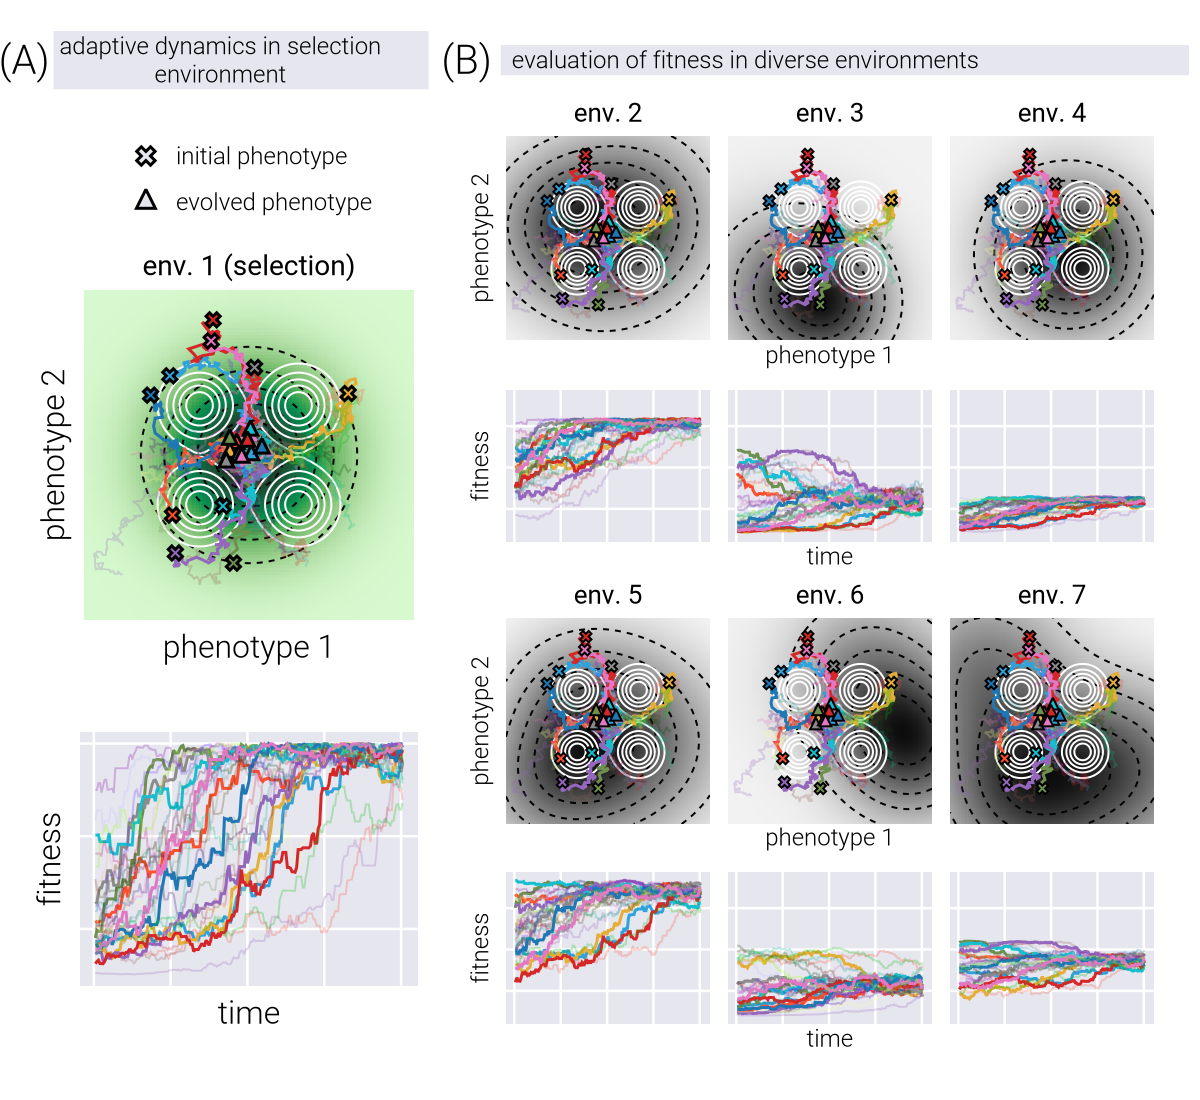
\includegraphics[keepaspectratio]{./fig/supplementary/figSI_02_kimura.pdf}}

}

\caption{\label{fig-02-kimura}\textbf{Evolutionary dynamics on phenotype
space with Metropolis-Kimura dynamics}. (A) Top: Metropolis-like
evolutionary dynamics on phenotype space. Each line represents the
trajectory of a lineage as it evolves over time, with crosses and
triangles denoting the initial phenotypic coordinate of a few selected
lineages. Note that trajectories tend to move towards higher fitness
values, avoiding low genotype-to-phenotype density regions. Bottom:
Fitness over time of the same trajectories shown above. (B) The same
trajectories shown in (A) overlaid on different fitness maps determined
by different environments. Although the phenotypic coordinates of the
genotypes remain the same (top panels), the resulting fitness readouts
change as the topography of the environment-dependent fitness landscape
changes (bottom panels).}

\end{figure}%

\paragraph{Figure 4 Main Text}\label{figure-4-main-text}

\begin{figure}

\centering{

\pandocbounded{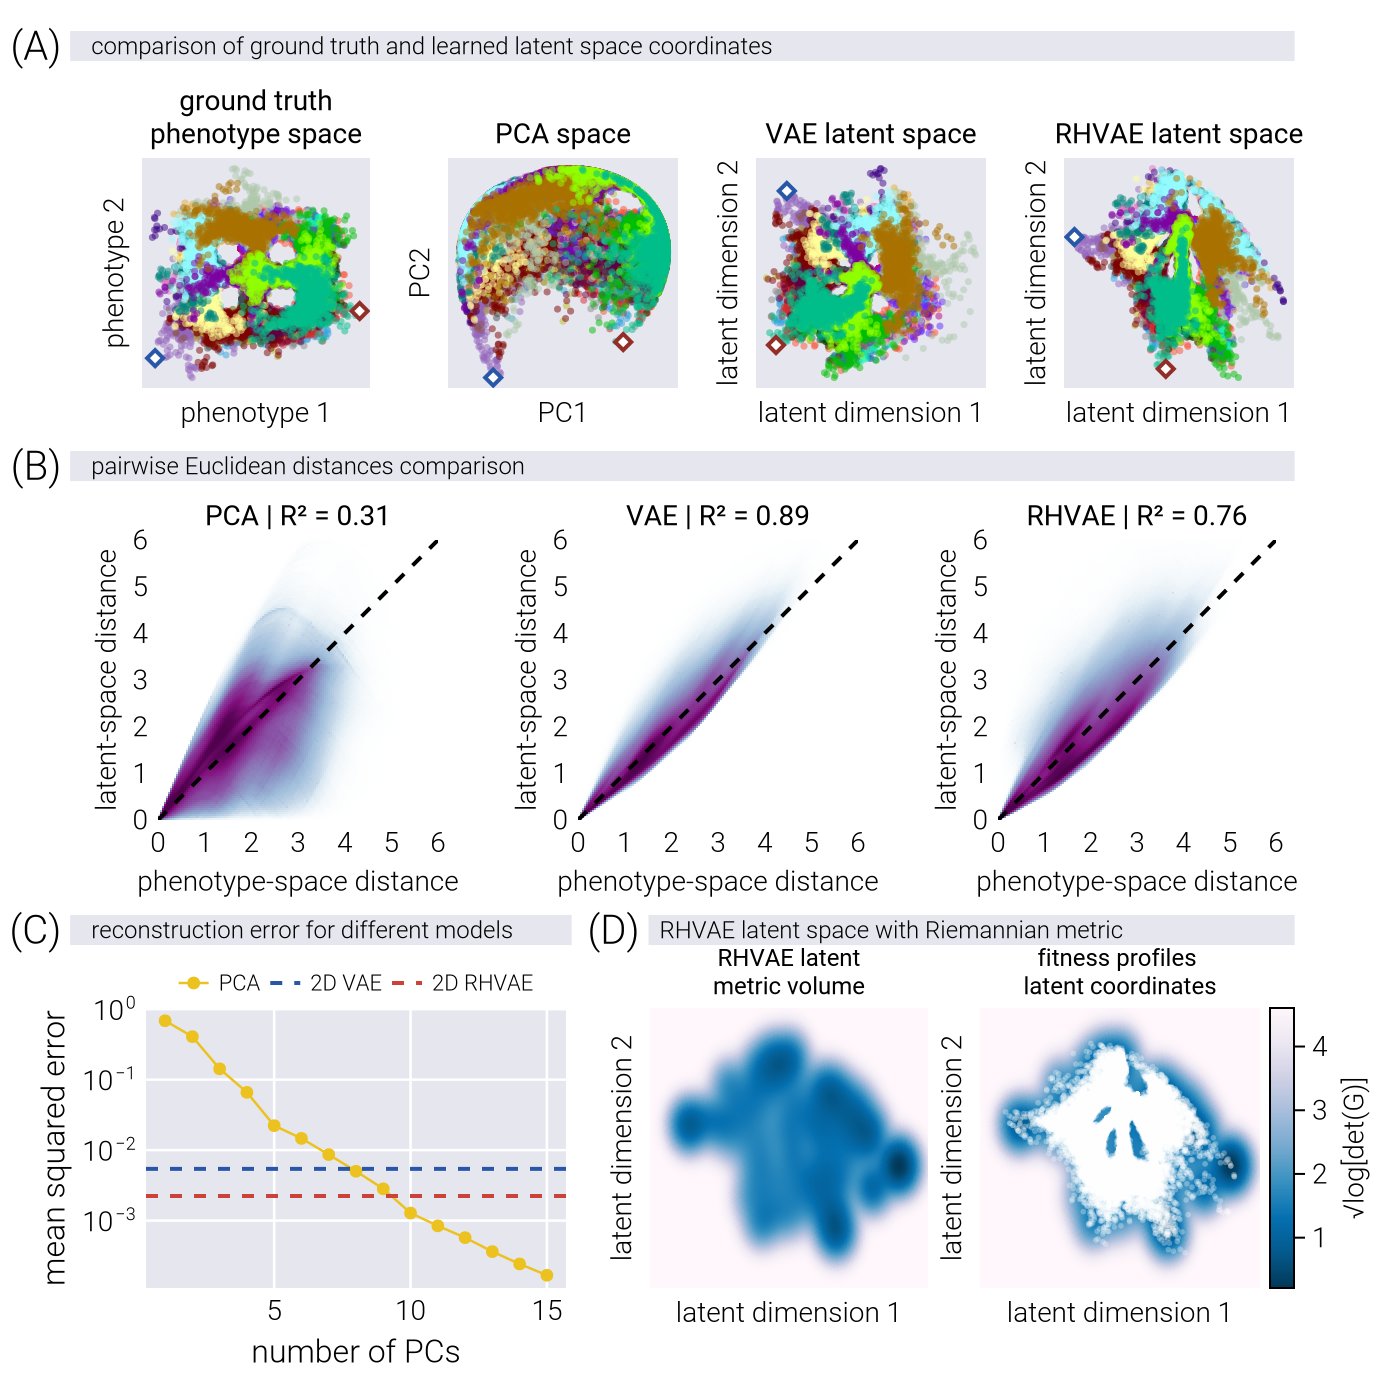
\includegraphics[keepaspectratio]{./fig/supplementary/figSI_04_kimura.pdf}}

}

\caption{\label{fig-04-kimura}\textbf{Geometry-informed latent space
captures phenotypic structure and improves reconstruction accuracy}. (A)
Latent space coordinates of simulated fitness profiles colored by
lineage, after alignment with the ground truth phenotype space using
Procrustes analysis. The RHVAE better preserves phenotypic relationships
than PCA or vanilla VAE, as evidenced by the highlighted points (diamond
markers). (B) Comparison of all pairwise Euclidean distances between
genotypes in the ground truth phenotypic space versus the different
latent spaces, showing RHVAE better preserves the original distances.
Given the large number of data points and the even larger number of
pairwise comparisons, the data are shown as a smear rather than single
points. (C) Reconstruction error (MSE) comparison showing 2D-RHVAE
achieves accuracy comparable to a 10-dimensional PCA model. (D) Metric
volume visualization of the RHVAE latent space (left) and with projected
data points (right), revealing regions of high curvature that correspond
to areas of low genotype-phenotype density in the simulation.}

\end{figure}%

\paragraph{Figure 5 Main Text}\label{figure-5-main-text}

\begin{figure}

\centering{

\pandocbounded{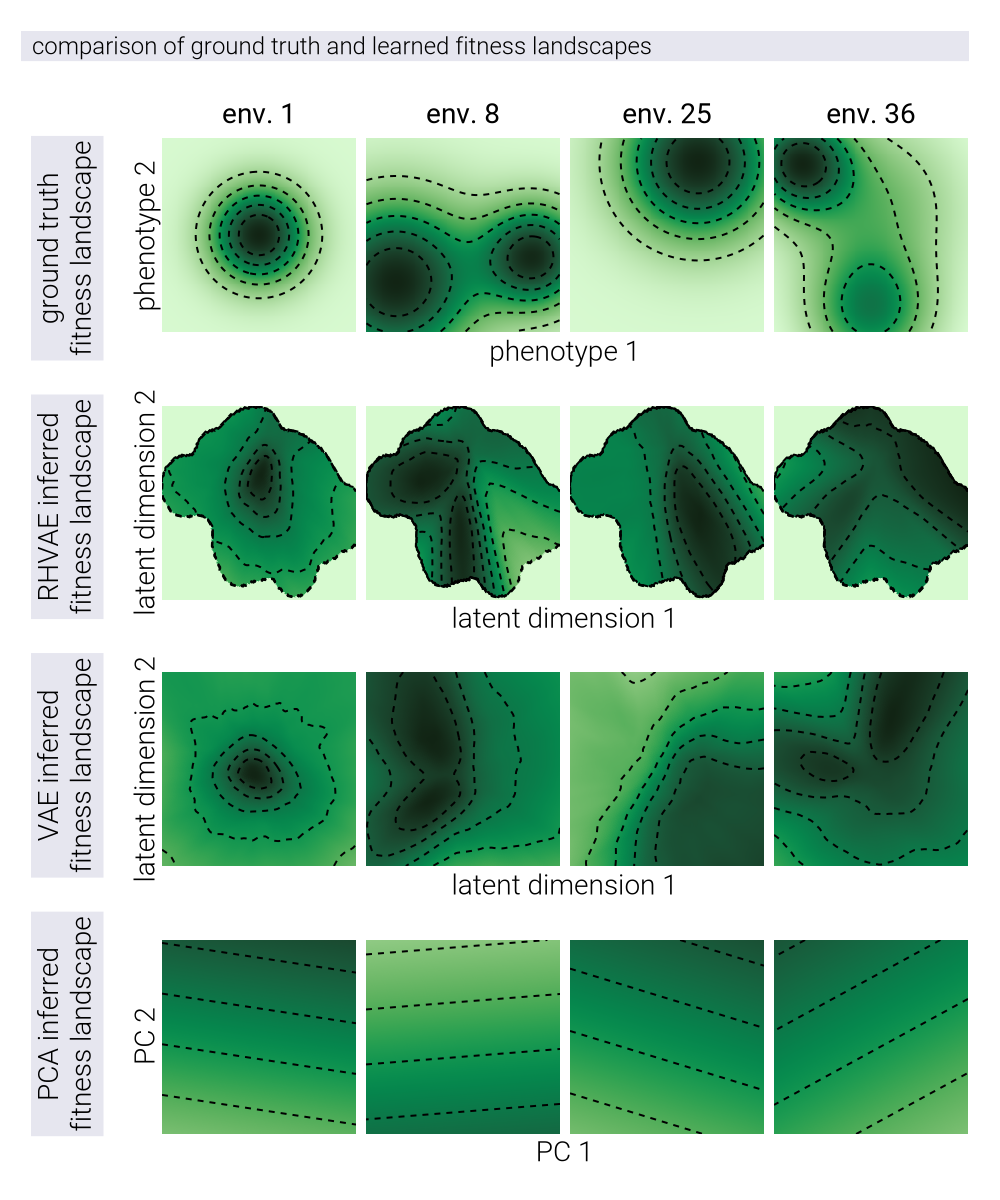
\includegraphics[keepaspectratio]{./fig/supplementary/figSI_05_kimura.pdf}}

}

\caption{\label{fig-05-kimura}\textbf{Geometry-informed latent space
enables accurate reconstruction of complex fitness landscapes}.
Comparison of ground truth and reconstructed fitness landscapes across
multiple environments. The first row shows examples of the original
simulated fitness landscapes used to generate the data. Subsequent rows
show reconstructions using the RHVAE (second row), VAE (third row), and
PCA (fourth row) models. The RHVAE accurately captures the underlying
topography, including the number and relative positions of fitness
peaks. While the VAE captures general landscape shapes, it lacks a
geometric metric to define prediction reliability regions. PCA fails to
represent the nonlinear structure of the landscapes, demonstrating the
limitations of linear dimensionality reduction for complex fitness
landscape reconstruction.}

\end{figure}%

% Print supplemental references changing the title
\printbibliography[title={Reference},
section=\therefsection]
\end{refsection}



\end{document}
